% Chapter 6

\chapter{Results} % Main chapter title
\section{Charged Track $v_{2}$}
Here I present measurements of elliptic flow in $\sqrt{s_{NN}}=200$ GeV d+Au collisions. Since the flattening the event plane redistributes the event plane distribution, the unidentified charged track flow can be measured directly from plots of $d\phi$. Recall that the Fourier coefficients parameterize the shape of the azimuthal hydrodynamic flow by describing it as a superposition of cosine harmonics:
\begin{equation}
\frac{d^{2}N}{dp^{2}} \propto v_0 + v_1 \cos\big(\phi - \Psi_{r}\big) + v_2 \cos\big(2(\phi - \Psi_{r})\big) + v_3 \cos\big(3(\phi - \Psi_{r})\big) \cdots
\end{equation}
where $v_0$, $v_1$, $v_2$, and $v_3$ are the values that scale the amount of spherical, directed, elliptic, and triangular flow respectively, and are indicative of collective behavior of the nuclear matter. To measure the elliptic flow we count number of tracks in bins of $d\phi$ and fit this with a function of the form:
\begin{equation}
\label{v2fitfn}
f(x) = A [1 + B \cos 2x]
\end{equation}
where A is a term that accounts for an overall shift in the number of tracks due to statistics and B is our $v_2$. Due to the asymmetric nature of d+Au collisions, event plane calculations are significantly better on the Au going side, because of this, the following plots (figures \ref{fig:Ndphicent0}-\ref{fig:Ndphicent3}) were made using the BBC South determination of the event plane. They are binned in 5\% bins of centrality up to 15\%, at which point statistics requires the remainder of data to be binned 10\%-25\%. This $d\phi$ plot can then be fit with the aforementioned cosine function to calculate the elliptic flow measurements vs centrality for all charged tracks which is shown in figure \ref{fig:alltrackv2}.


\begin{figure}[htbp!]
  \centering
    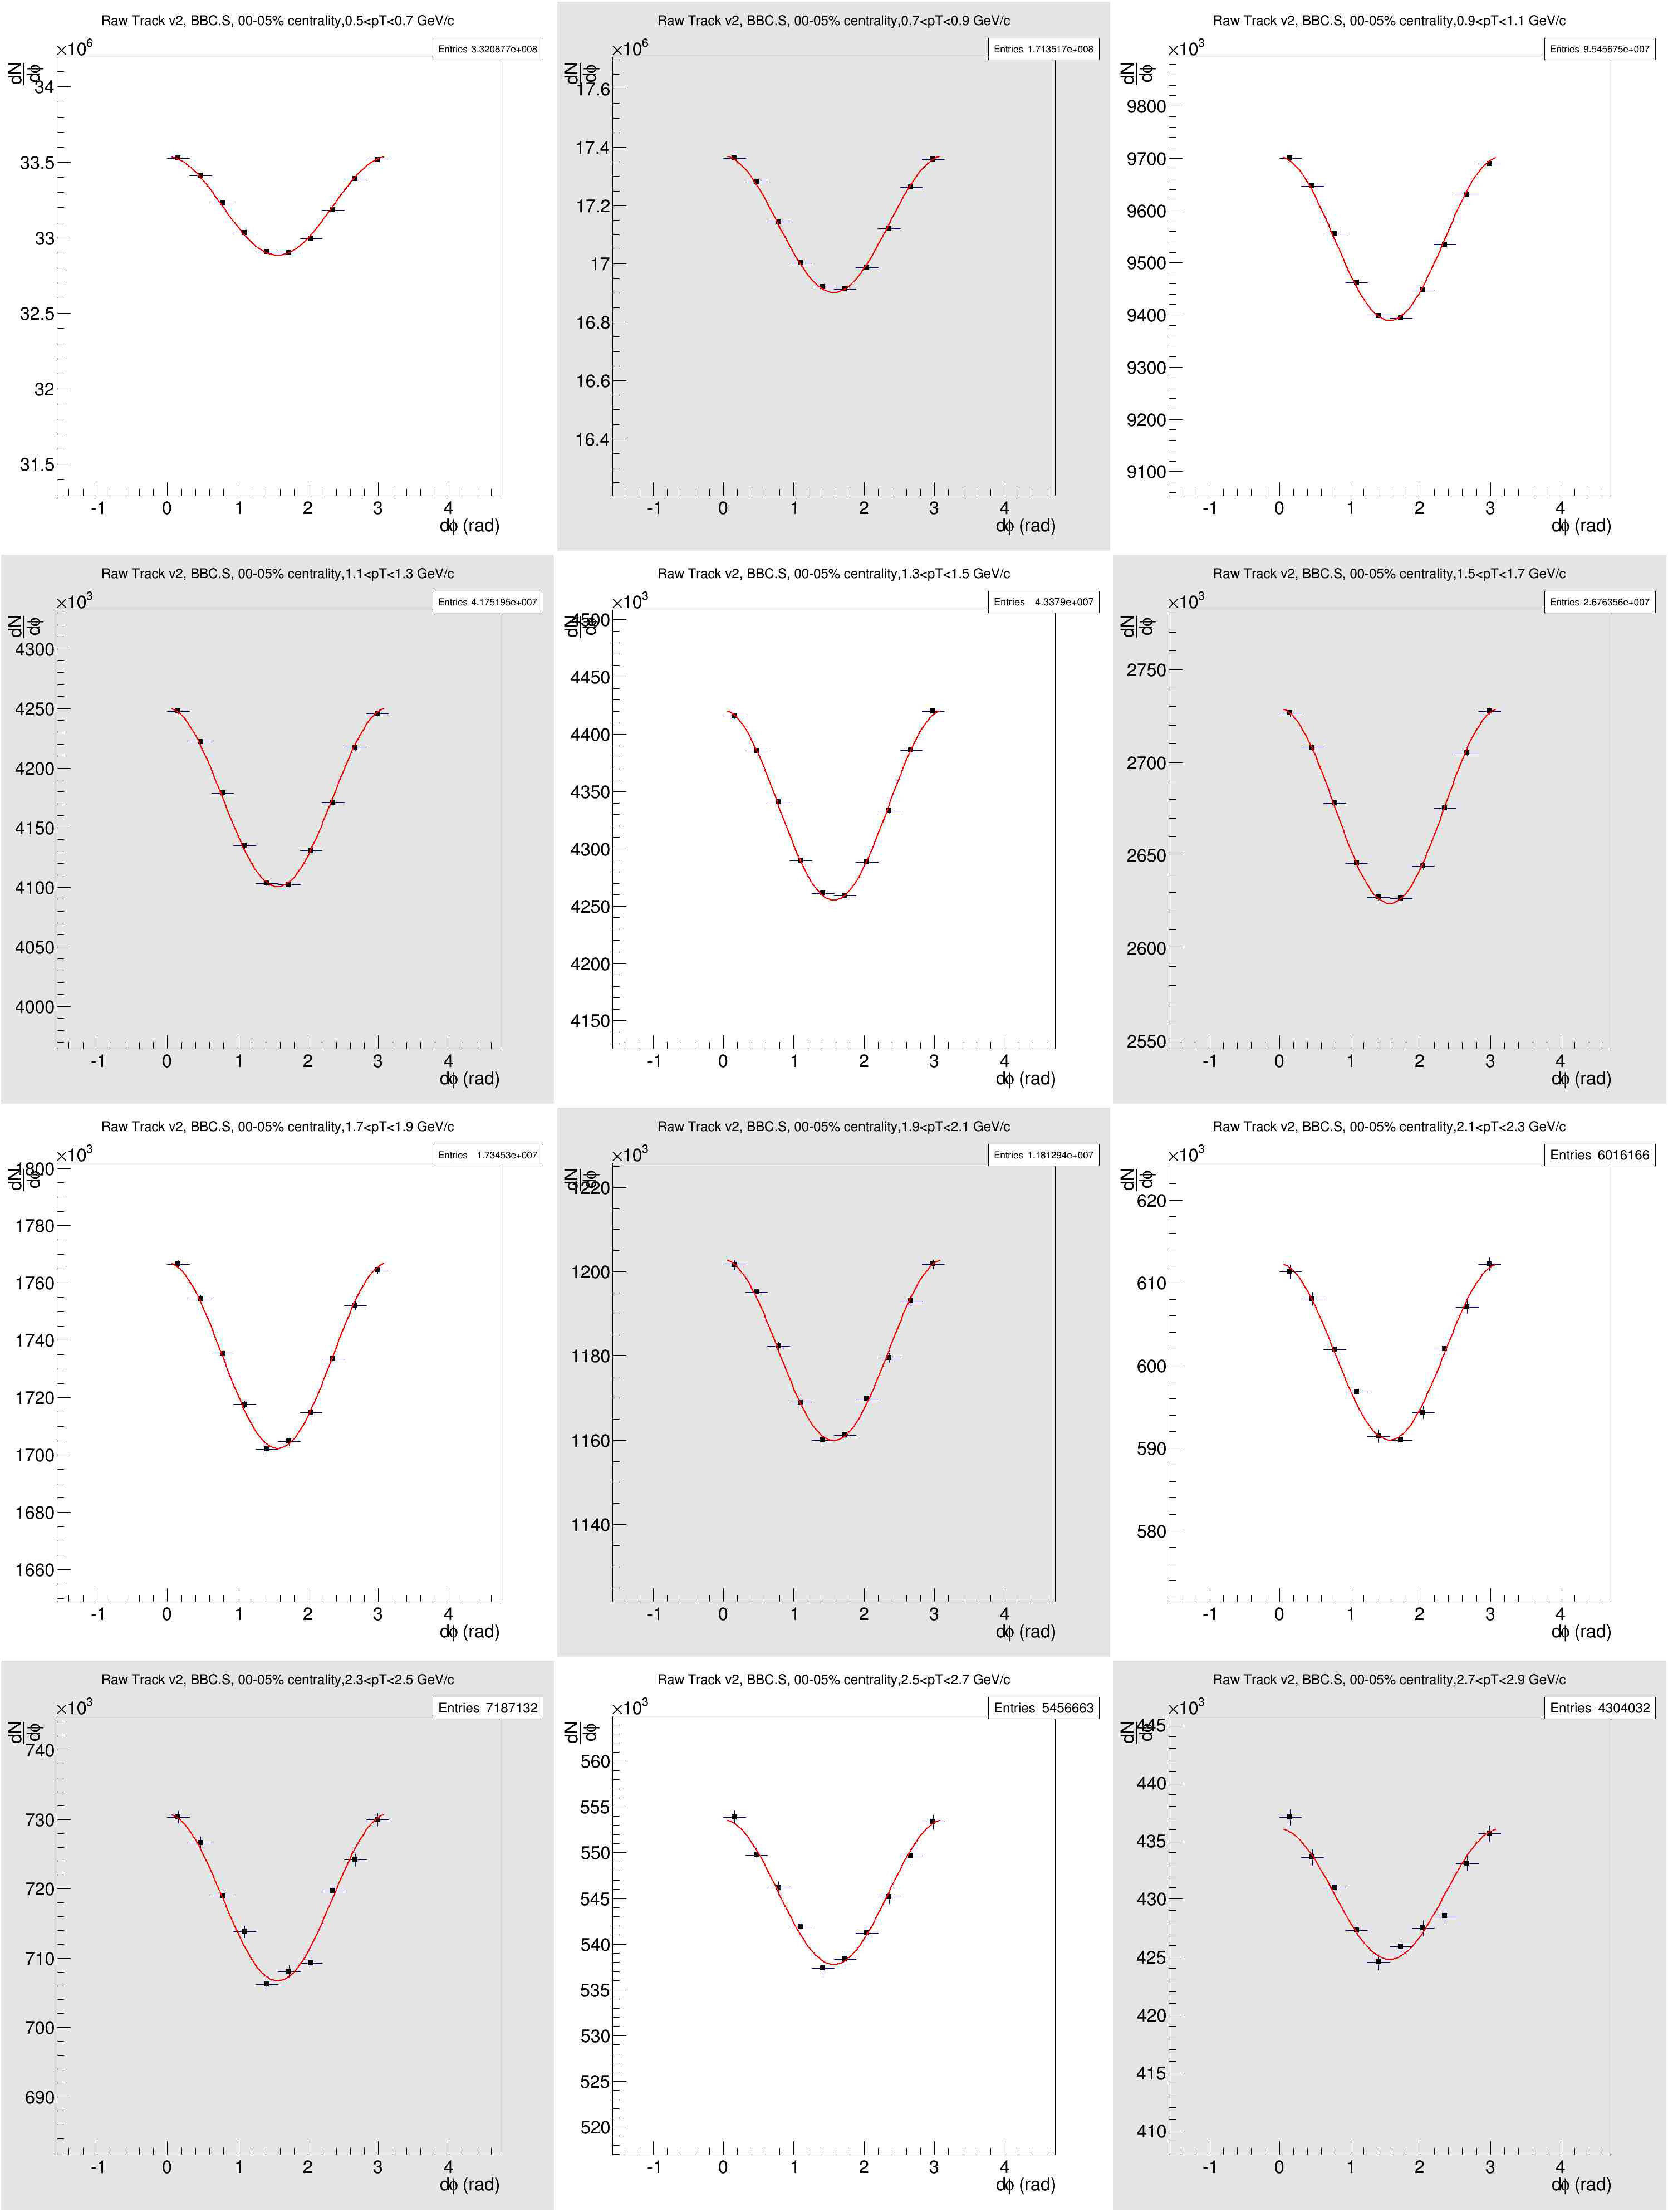
\includegraphics[width=1\textwidth]{chargedtrackv2/htrkdphi2bbcs_0.jpg}
    \rule{35em}{0.5pt}
  \caption[$\frac{dN}{d\phi}$ vs $d\phi$, 0-5\% centrality.]{$\frac{d^N}{d\phi}$ vs $d\phi$, 0-5\% centrality, each plot represents a 0.2 GeV slice in transverse momentum space.}
  \label{fig:Ndphicent0}
\end{figure}

\begin{figure}[htbp!]
  \centering
    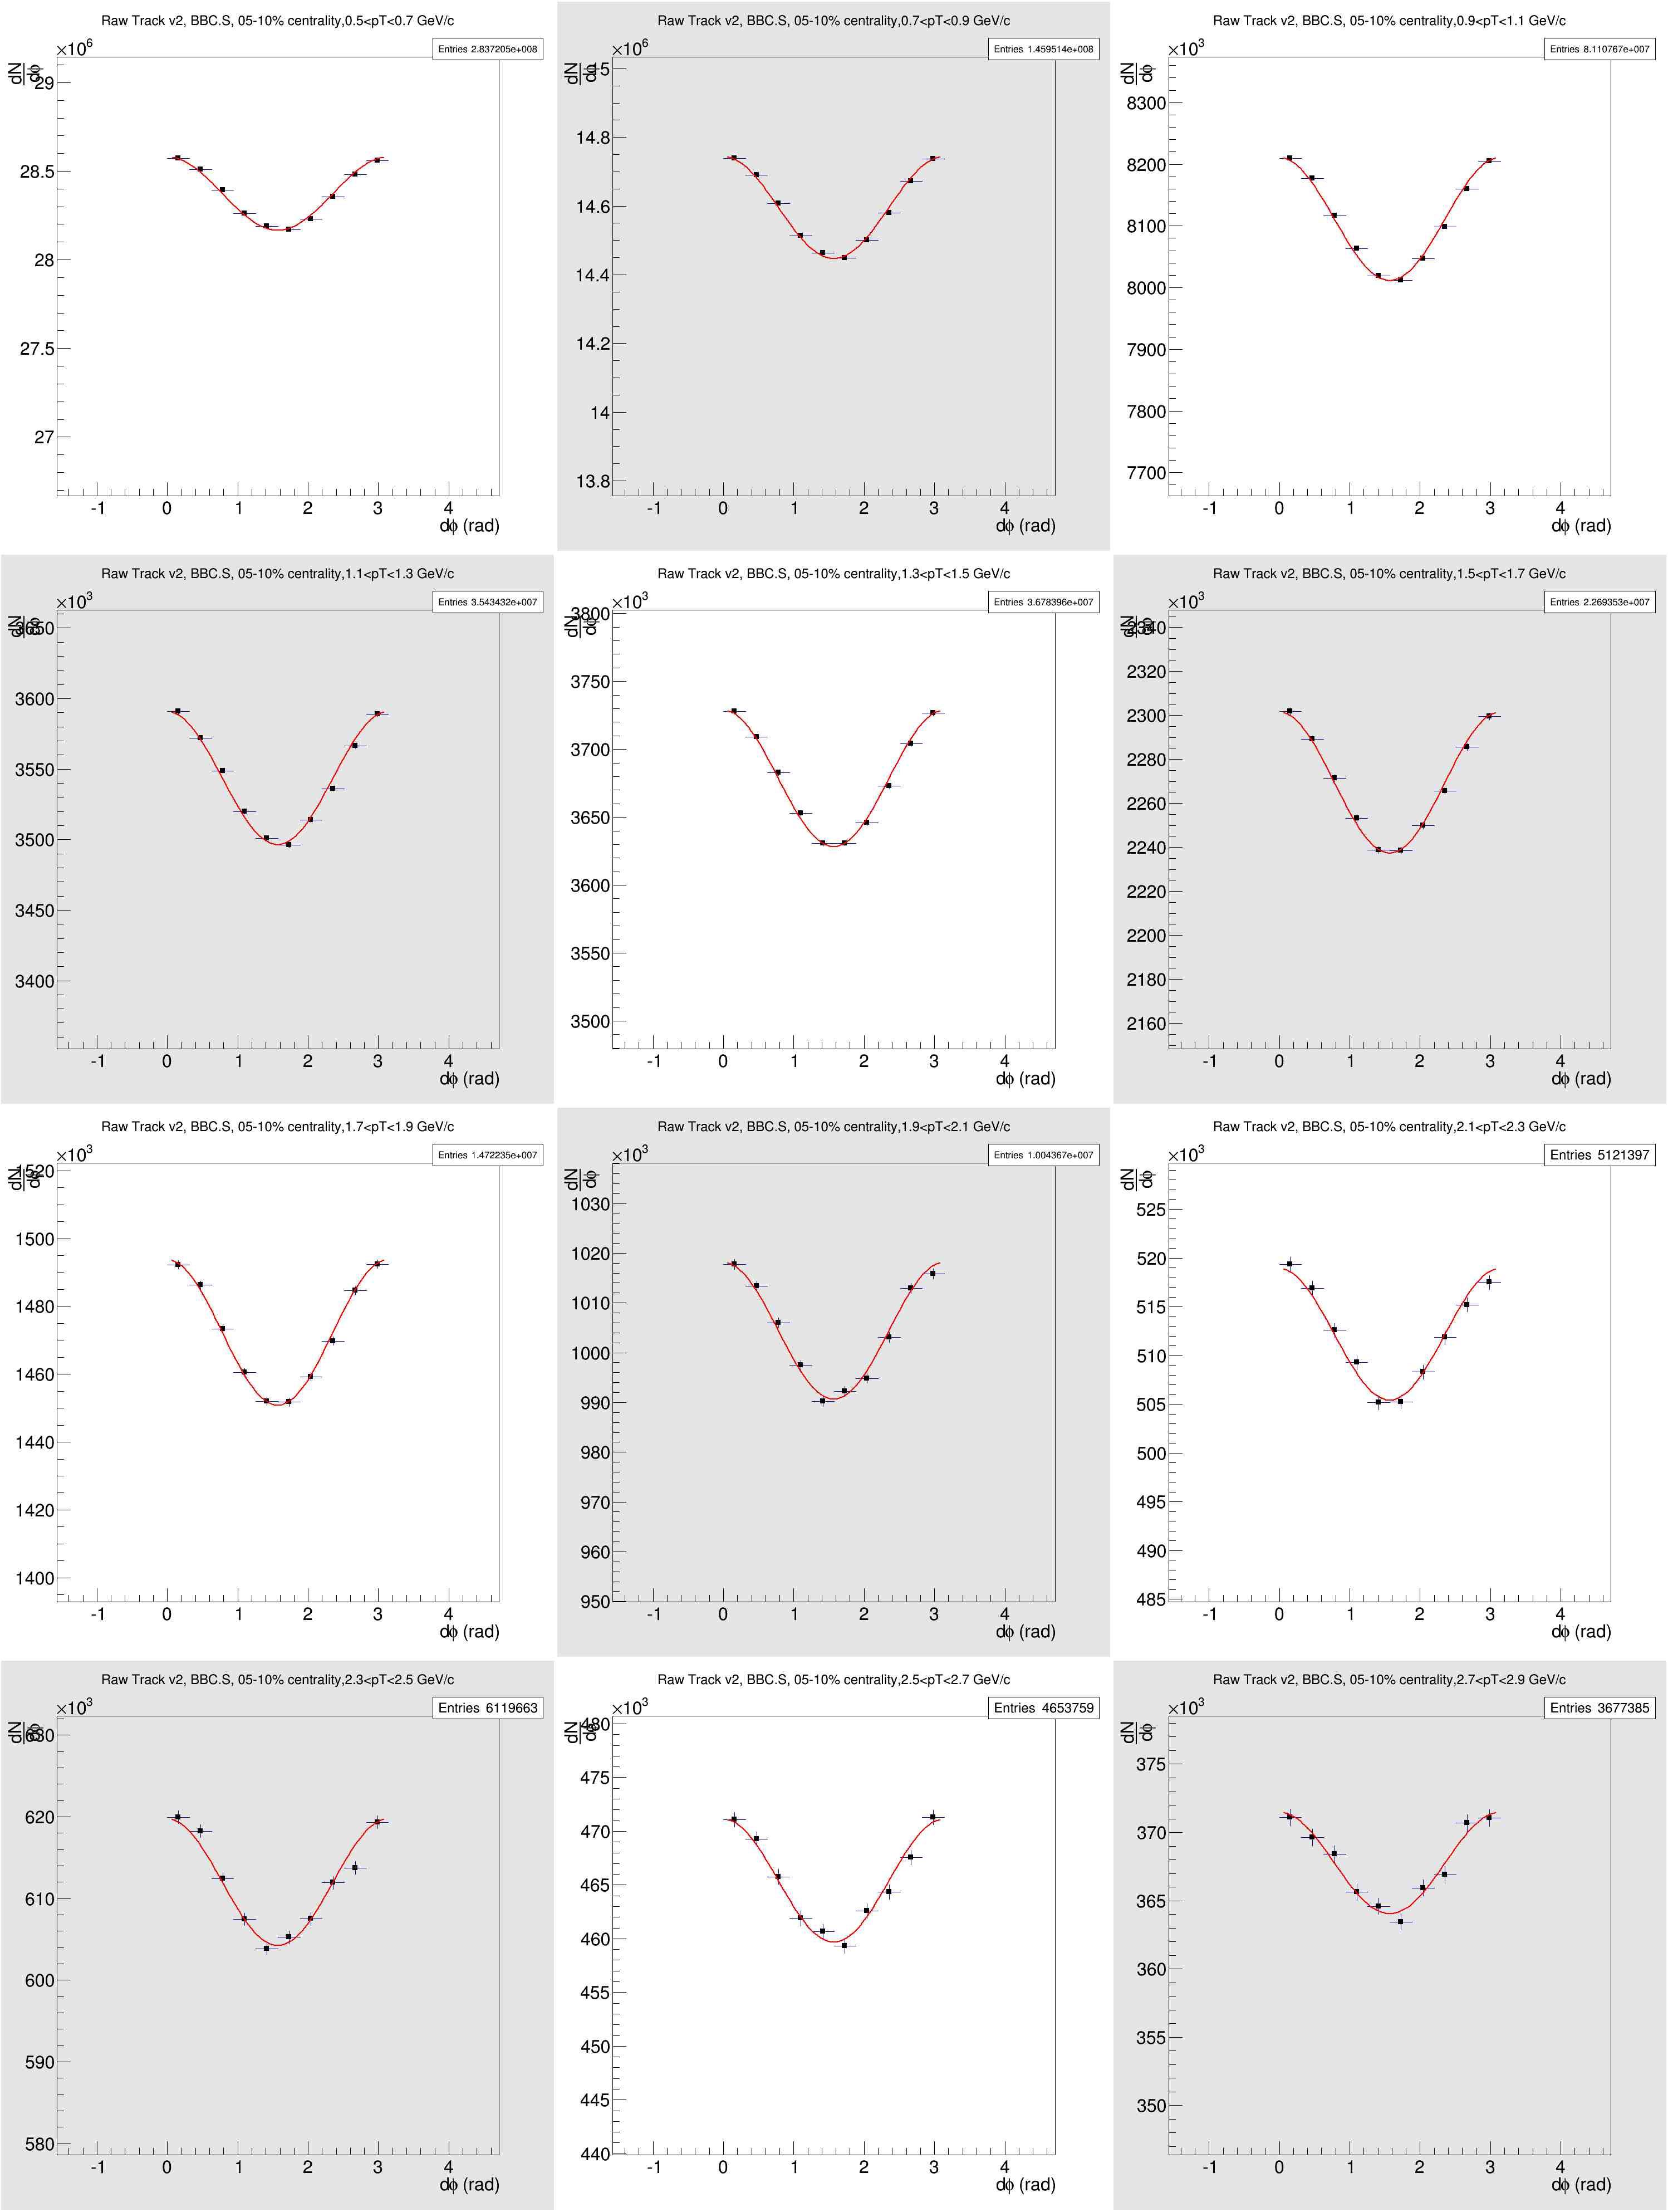
\includegraphics[width=1\textwidth]{chargedtrackv2/htrkdphi2bbcs_1.jpg}
    \rule{35em}{0.5pt}
  \caption[$\frac{dN}{d\phi}$ vs $d\phi$, 5-10\% centrality.]{$\frac{d^N}{d\phi}$ vs $d\phi$, 5-10\% centrality, each plot represents a 0.2 GeV slice in transverse momentum space.}
  \label{fig:Ndphicent1}
\end{figure}
\begin{figure}[htbp!]
  \centering
    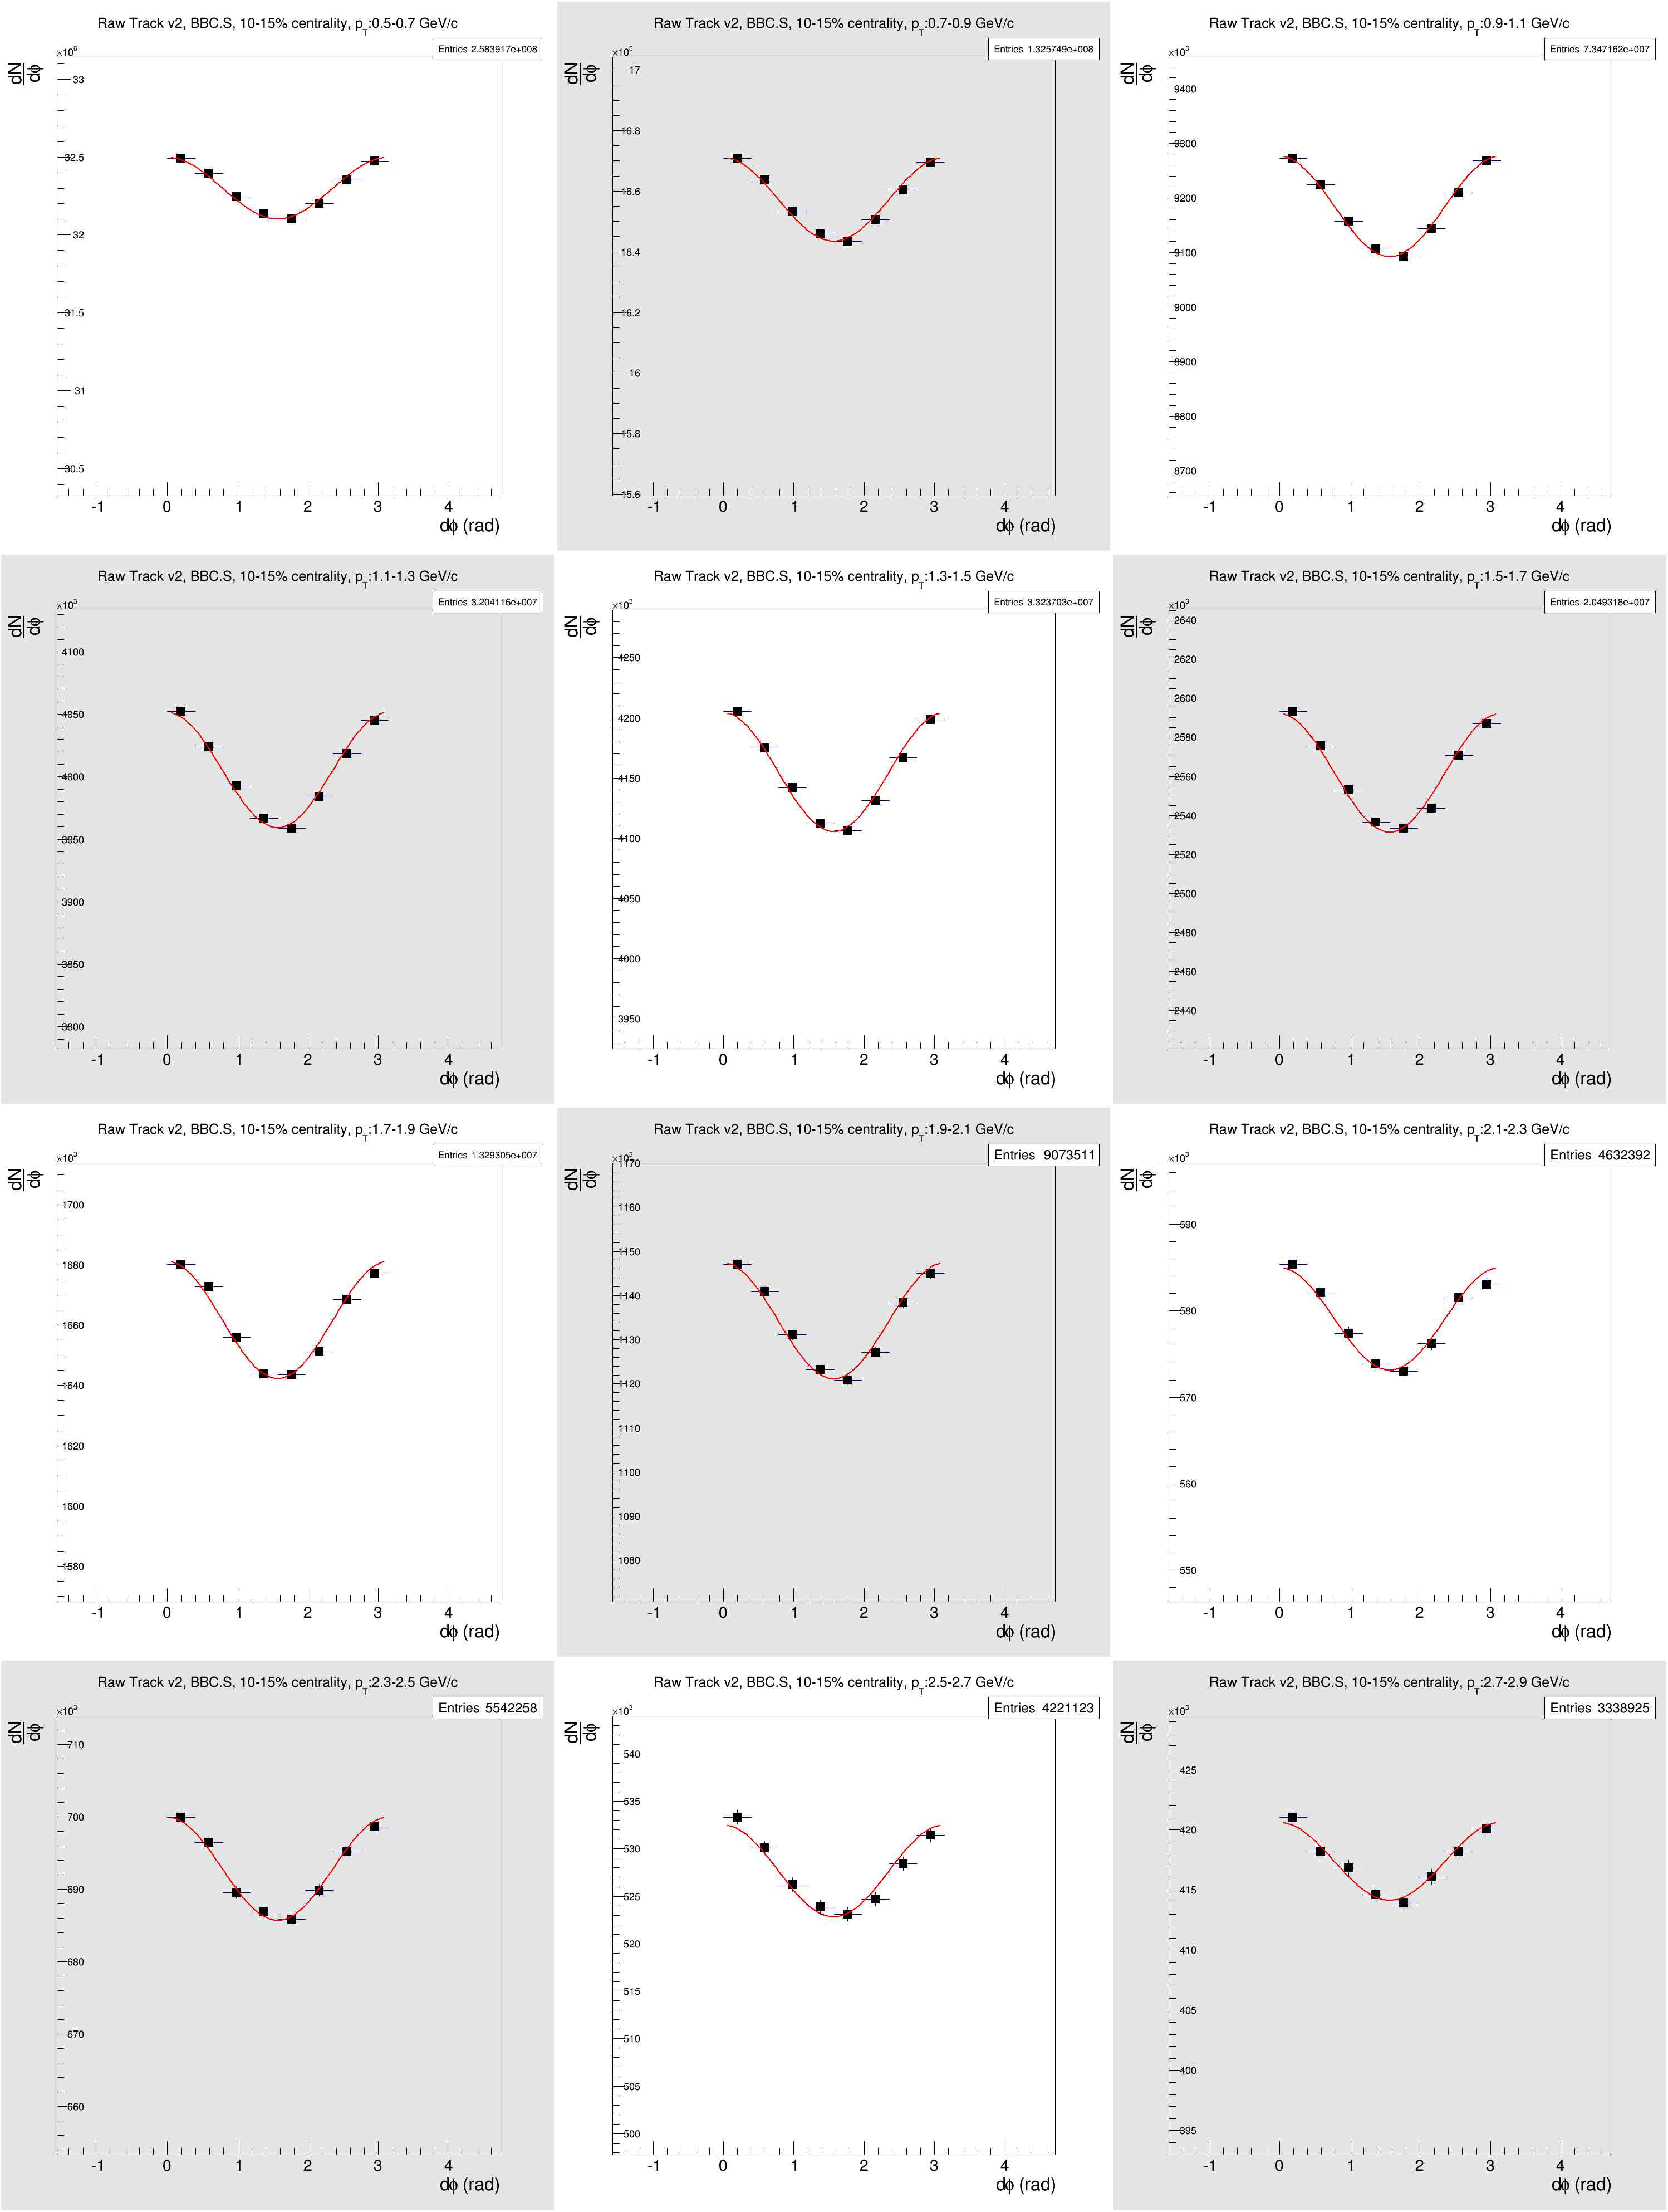
\includegraphics[width=1\textwidth]{chargedtrackv2/htrkdphi2bbcs_2.jpg}
    \rule{35em}{0.5pt}
  \caption[$\frac{dN}{d\phi}$ vs $d\phi$, 10-15\% centrality.]{$\frac{d^N}{d\phi}$ vs $d\phi$, 10-15\% centrality, each plot represents a 0.2 GeV slice in transverse momentum space.}
  \label{fig:Ndphicent2}
\end{figure}
\begin{figure}[htbp!]
  \centering
    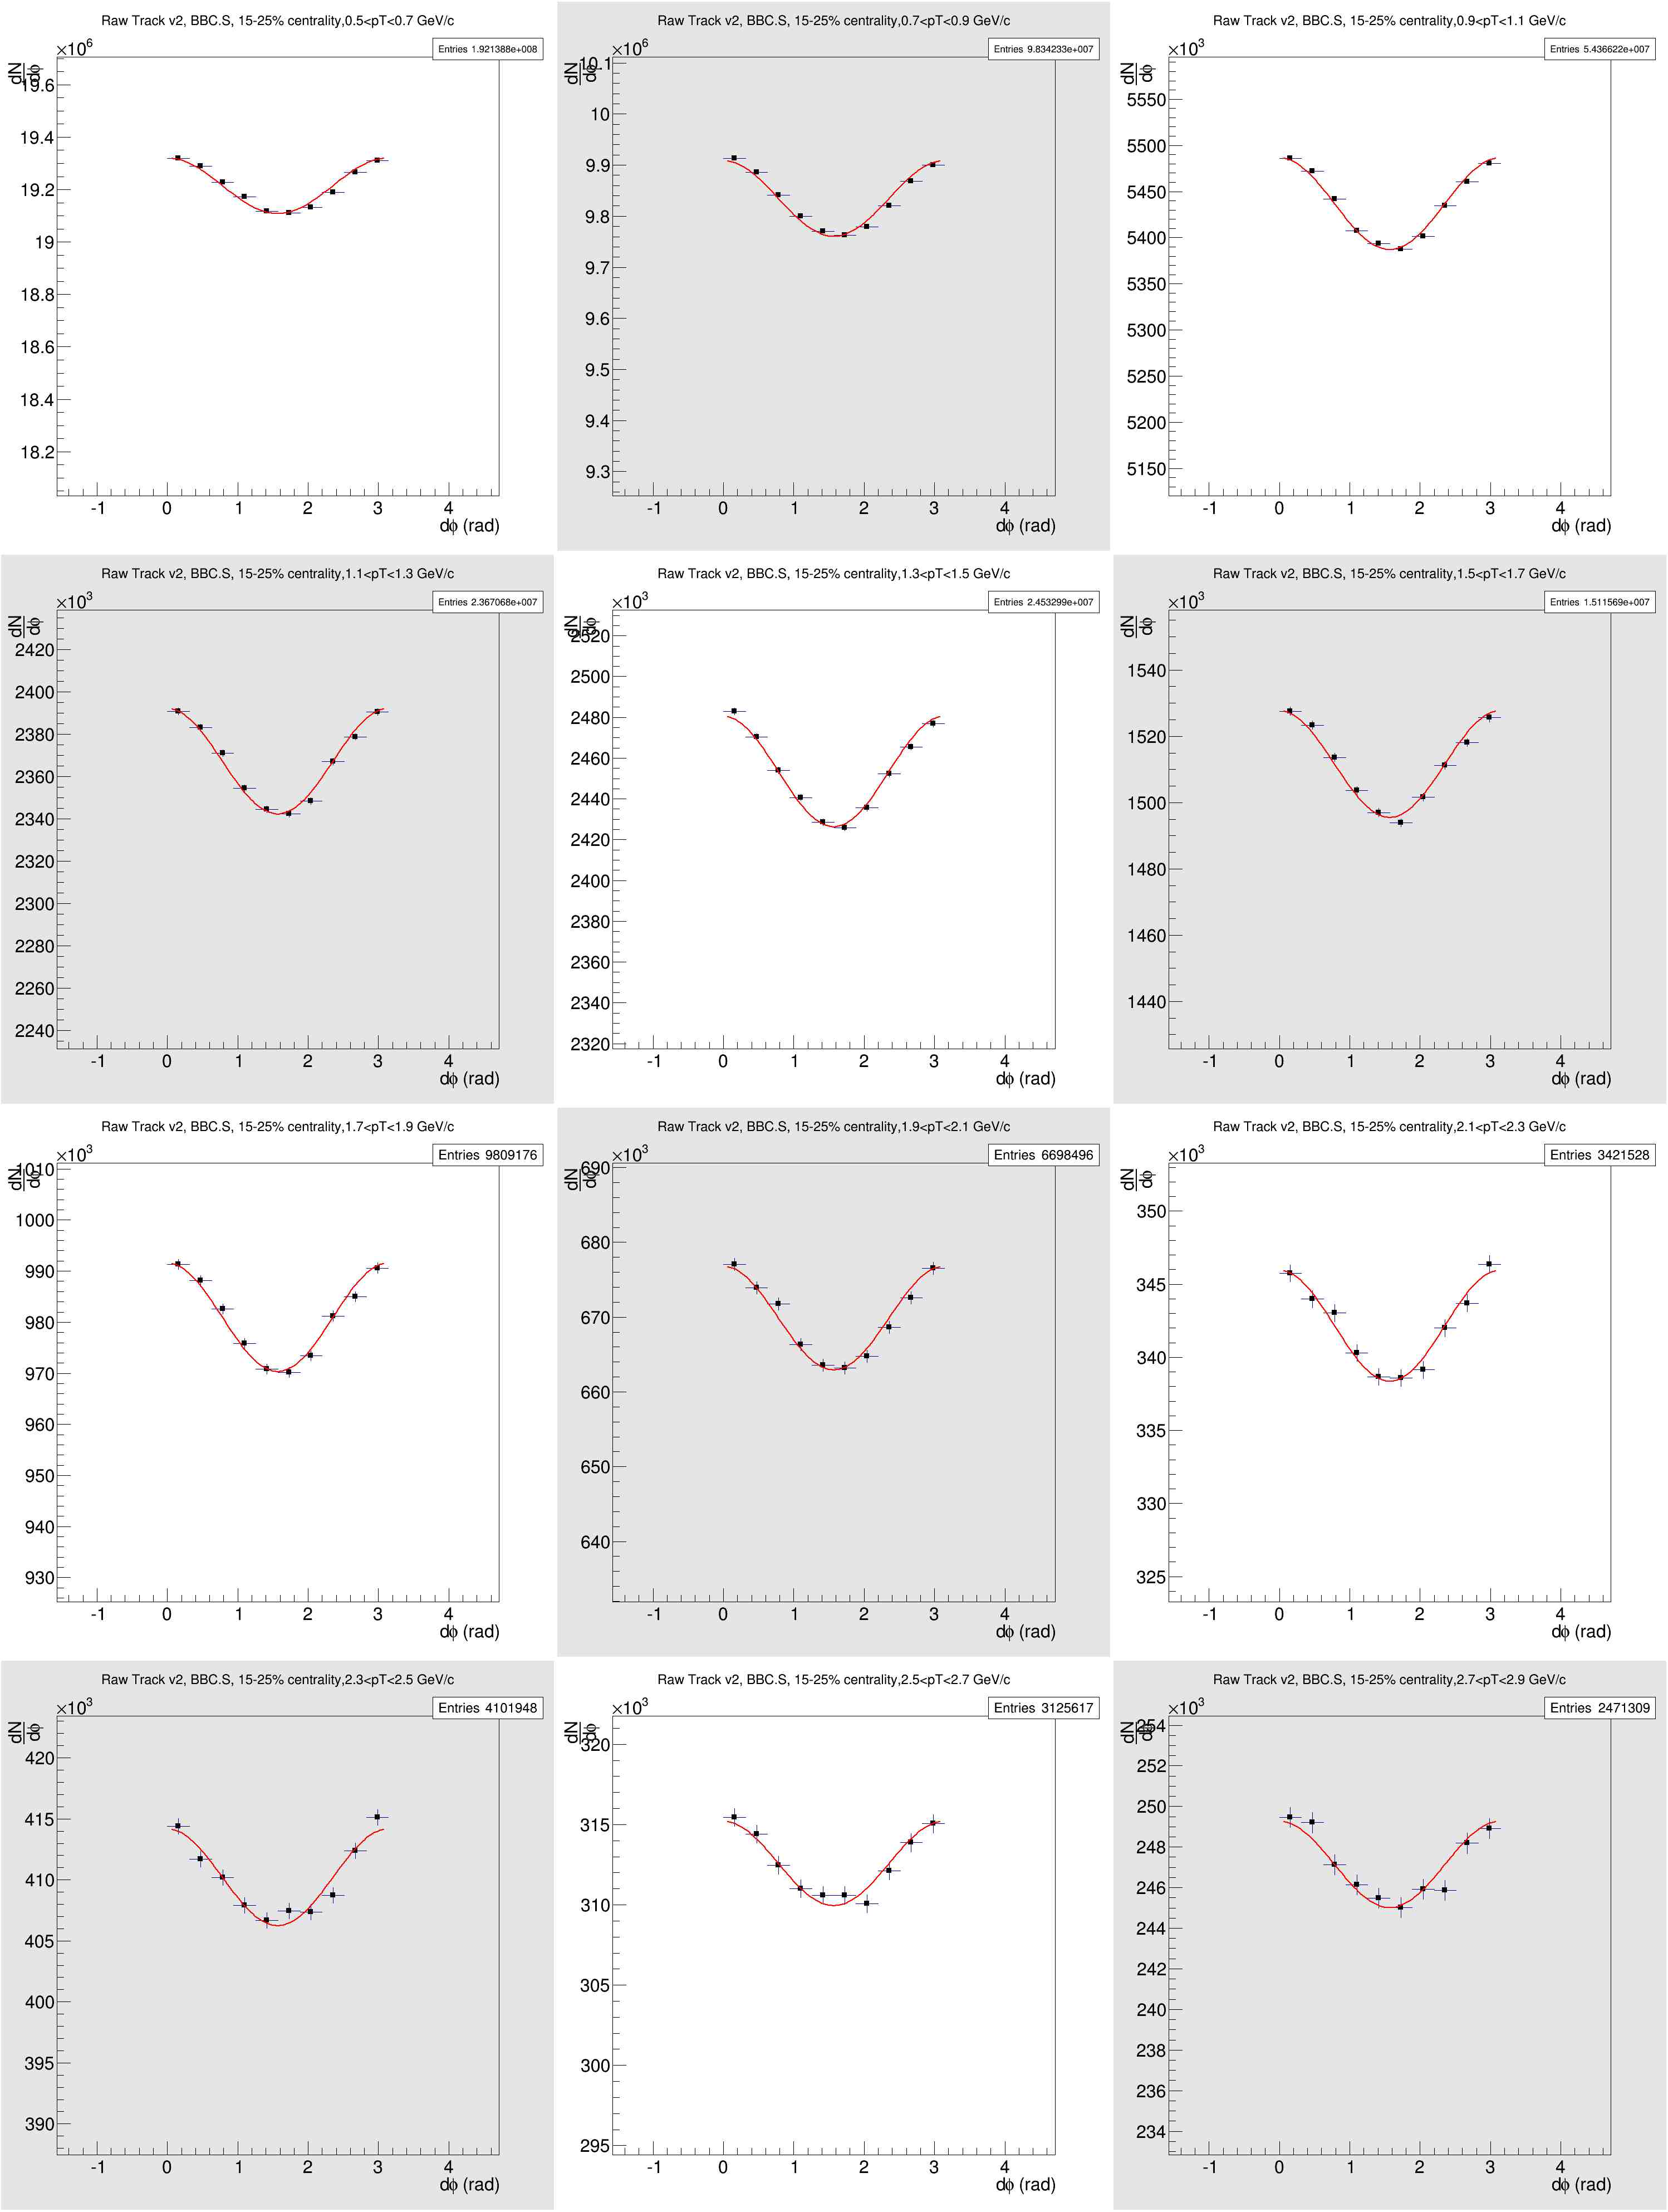
\includegraphics[width=1\textwidth]{chargedtrackv2/htrkdphi2bbcs_3.jpg}
    \rule{35em}{0.5pt}
  \caption[$\frac{dN}{d\phi}$ vs $d\phi$, 15-25\% centrality.]{$\frac{d^N}{d\phi}$ vs $d\phi$, 15-25\% centrality, each plot represents a 0.2 GeV slice in transverse momentum space.}
  \label{fig:Ndphicent3}
\end{figure}

\begin{figure}[htbp!]
  \centering
    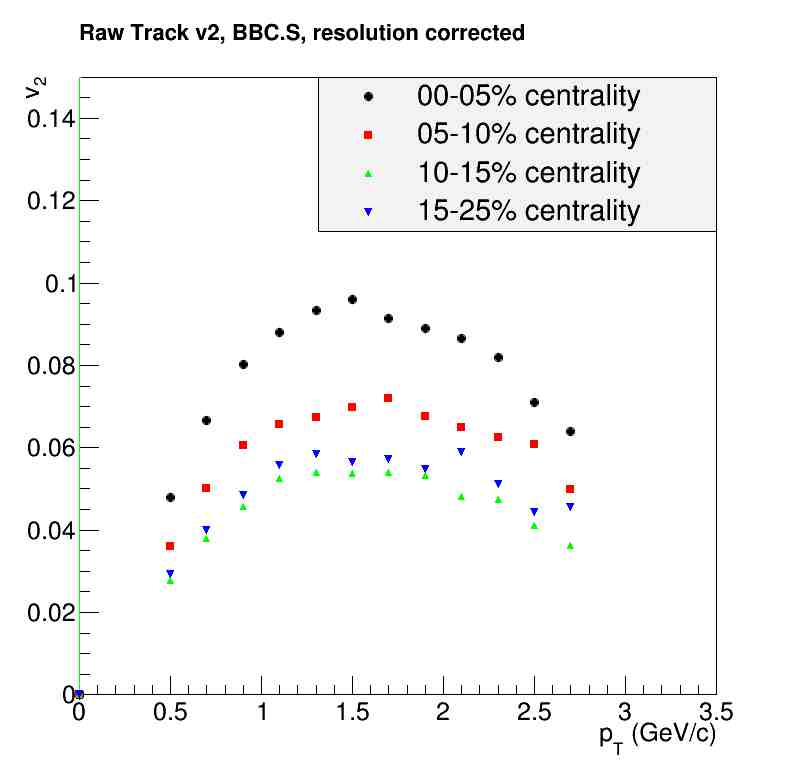
\includegraphics[width=0.7\textwidth]{chargedtrackv2/rawtrackv2_bbcNS.jpg}
    \rule{35em}{0.5pt}
  \caption[Charged track elliptic flow,$\sqrt{s_{NN}}=$200 GeV d+Au collisions]{Charged track elliptic flow,$\sqrt{s_{NN}}=$200 GeV d+Au collisions}
  \label{fig:alltrackv2}
\end{figure}
\clearpage
\section{Separating Particle Signals}
Following the flattening of the event plane and checking for calibration of the TOF detector, I can plot a 2-d histogram of $p_T$ vs $m^2$ following the method described in section \ref{sect:pidmethod} to identify the species of charged track hits in the TOF. In order to do a statistical analysis, these 2-d histograms will need to be ``sliced'' into a series of 1-d histograms in small bins of $p_T$ which will give a 3-peak histogram showing the signatures of the pion, kaon, and proton which are Gaussian in shape. The widths and heights of these particle peaks will change and overlap in various ways over the variance of $p_t$, because of this I will divide the $p_T$ range into three ranges which will be analyzed with different methods. The Gaussians are then integrated to calculate the particle yield for each species. Integration bounds can be set to increase track ID purity at the expense of statistics and vice versa. As a QA tool means and widths across each bin in $d\phi$ are plotted and set to be flat as there should not be a shift in either of those for a set bin of $p_T$. The yields from the integrated Gaussians are then fit with the Fourier function to determine the 2nd harmonic coefficient as per equation \ref{v2fitfn}.

\subsection{Single Gaussians}
For $p_T< 1.3$, there is enough separation between the pion, kaon, and proton signals to fit each particle peak with a single Gaussian. This will take the form:
\begin{equation}
f(x) = \frac{N_0}{\sqrt{2\pi \sigma^2}} e^{-\frac{(x-\mu)^2}{2\sigma^{2}}},
\end{equation}
where $\sigma$ is the width of the identified particle peak, $\mu$ is the location of the peak's mean along the x-axis, and $N_0$ is the height of the peak. The Gaussians are then integrated from $\mu-2\sigma$ to $\mu+2\sigma$ for each particle distribution, i.e. the number of particles of each type are counted out to two standard deviations around their mean mass. 

\newgeometry{top=2cm} 
\subsubsection{Single Gaussian fits, $p_T$=0.5-1.3 GeV/c, TOF.W, negative charged tracks}

\begin{figure}[H]
  \centering
    \begin{subfigure}{1\textwidth}
    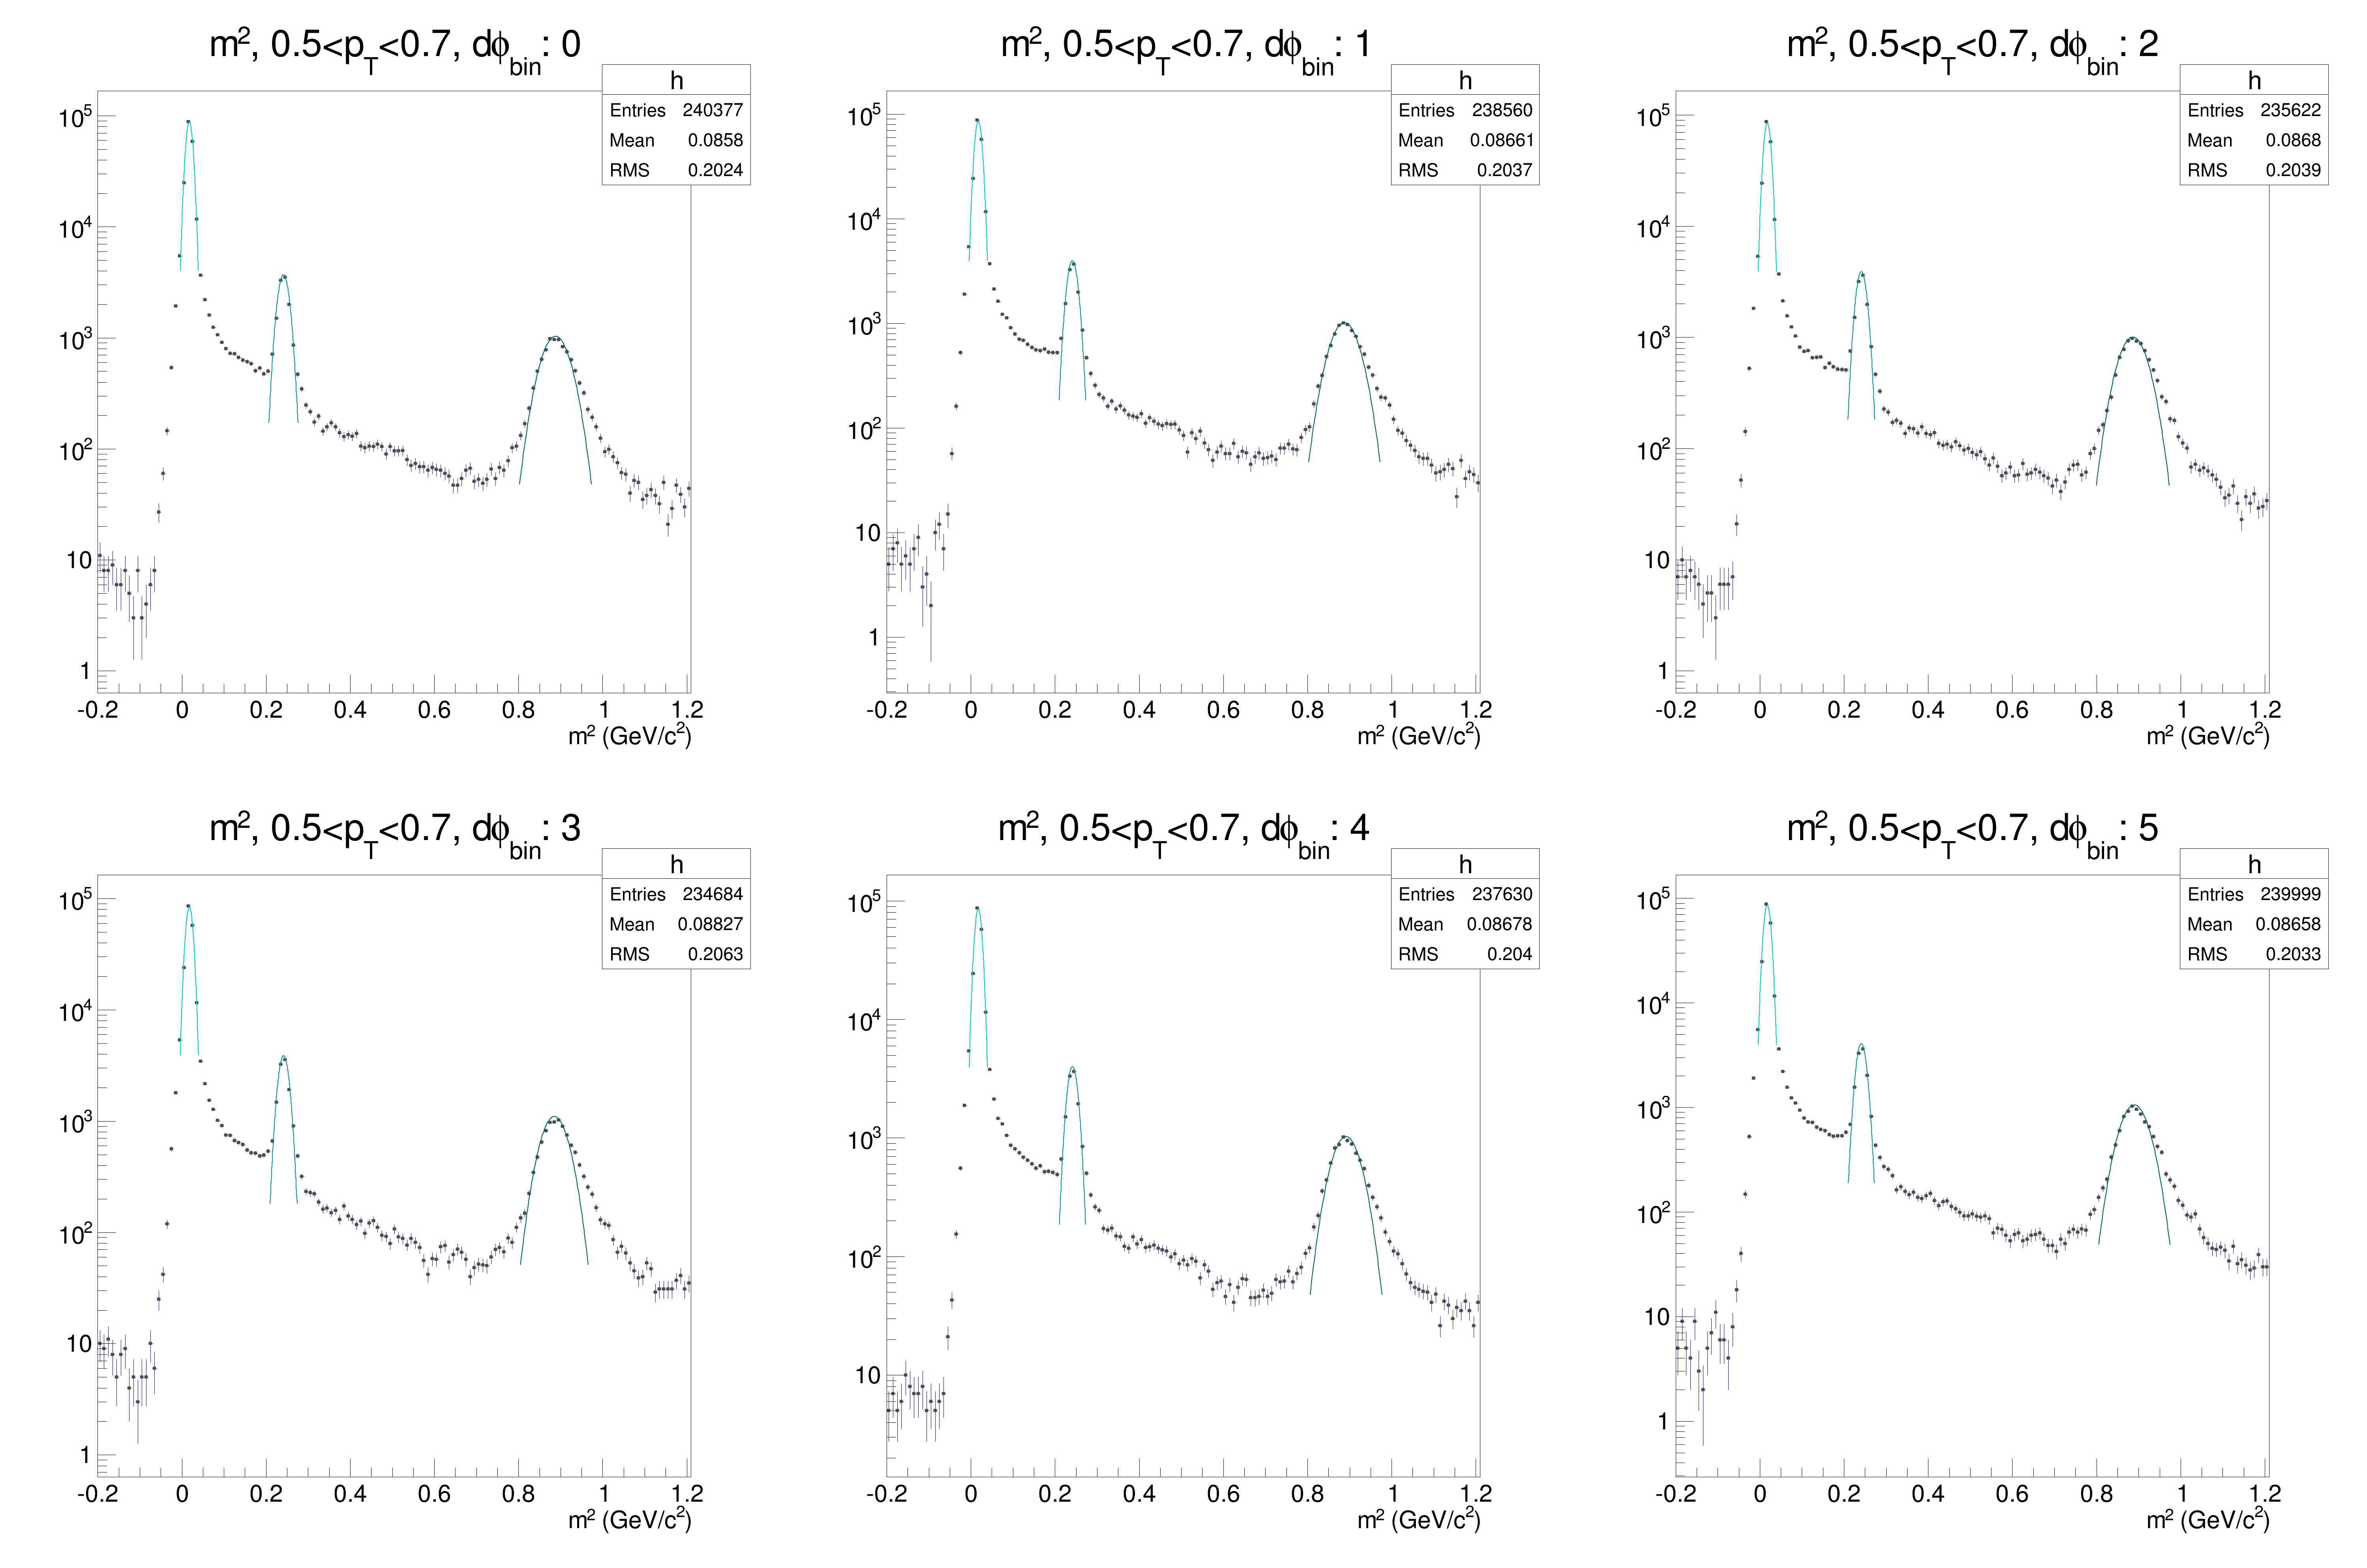
\includegraphics[width=1\textwidth]{lowptfits/yieldvsdphi_tof1_cent0_ch0_pT-5-7.jpg}
    \end{subfigure}
    \begin{subfigure}{1\textwidth}
    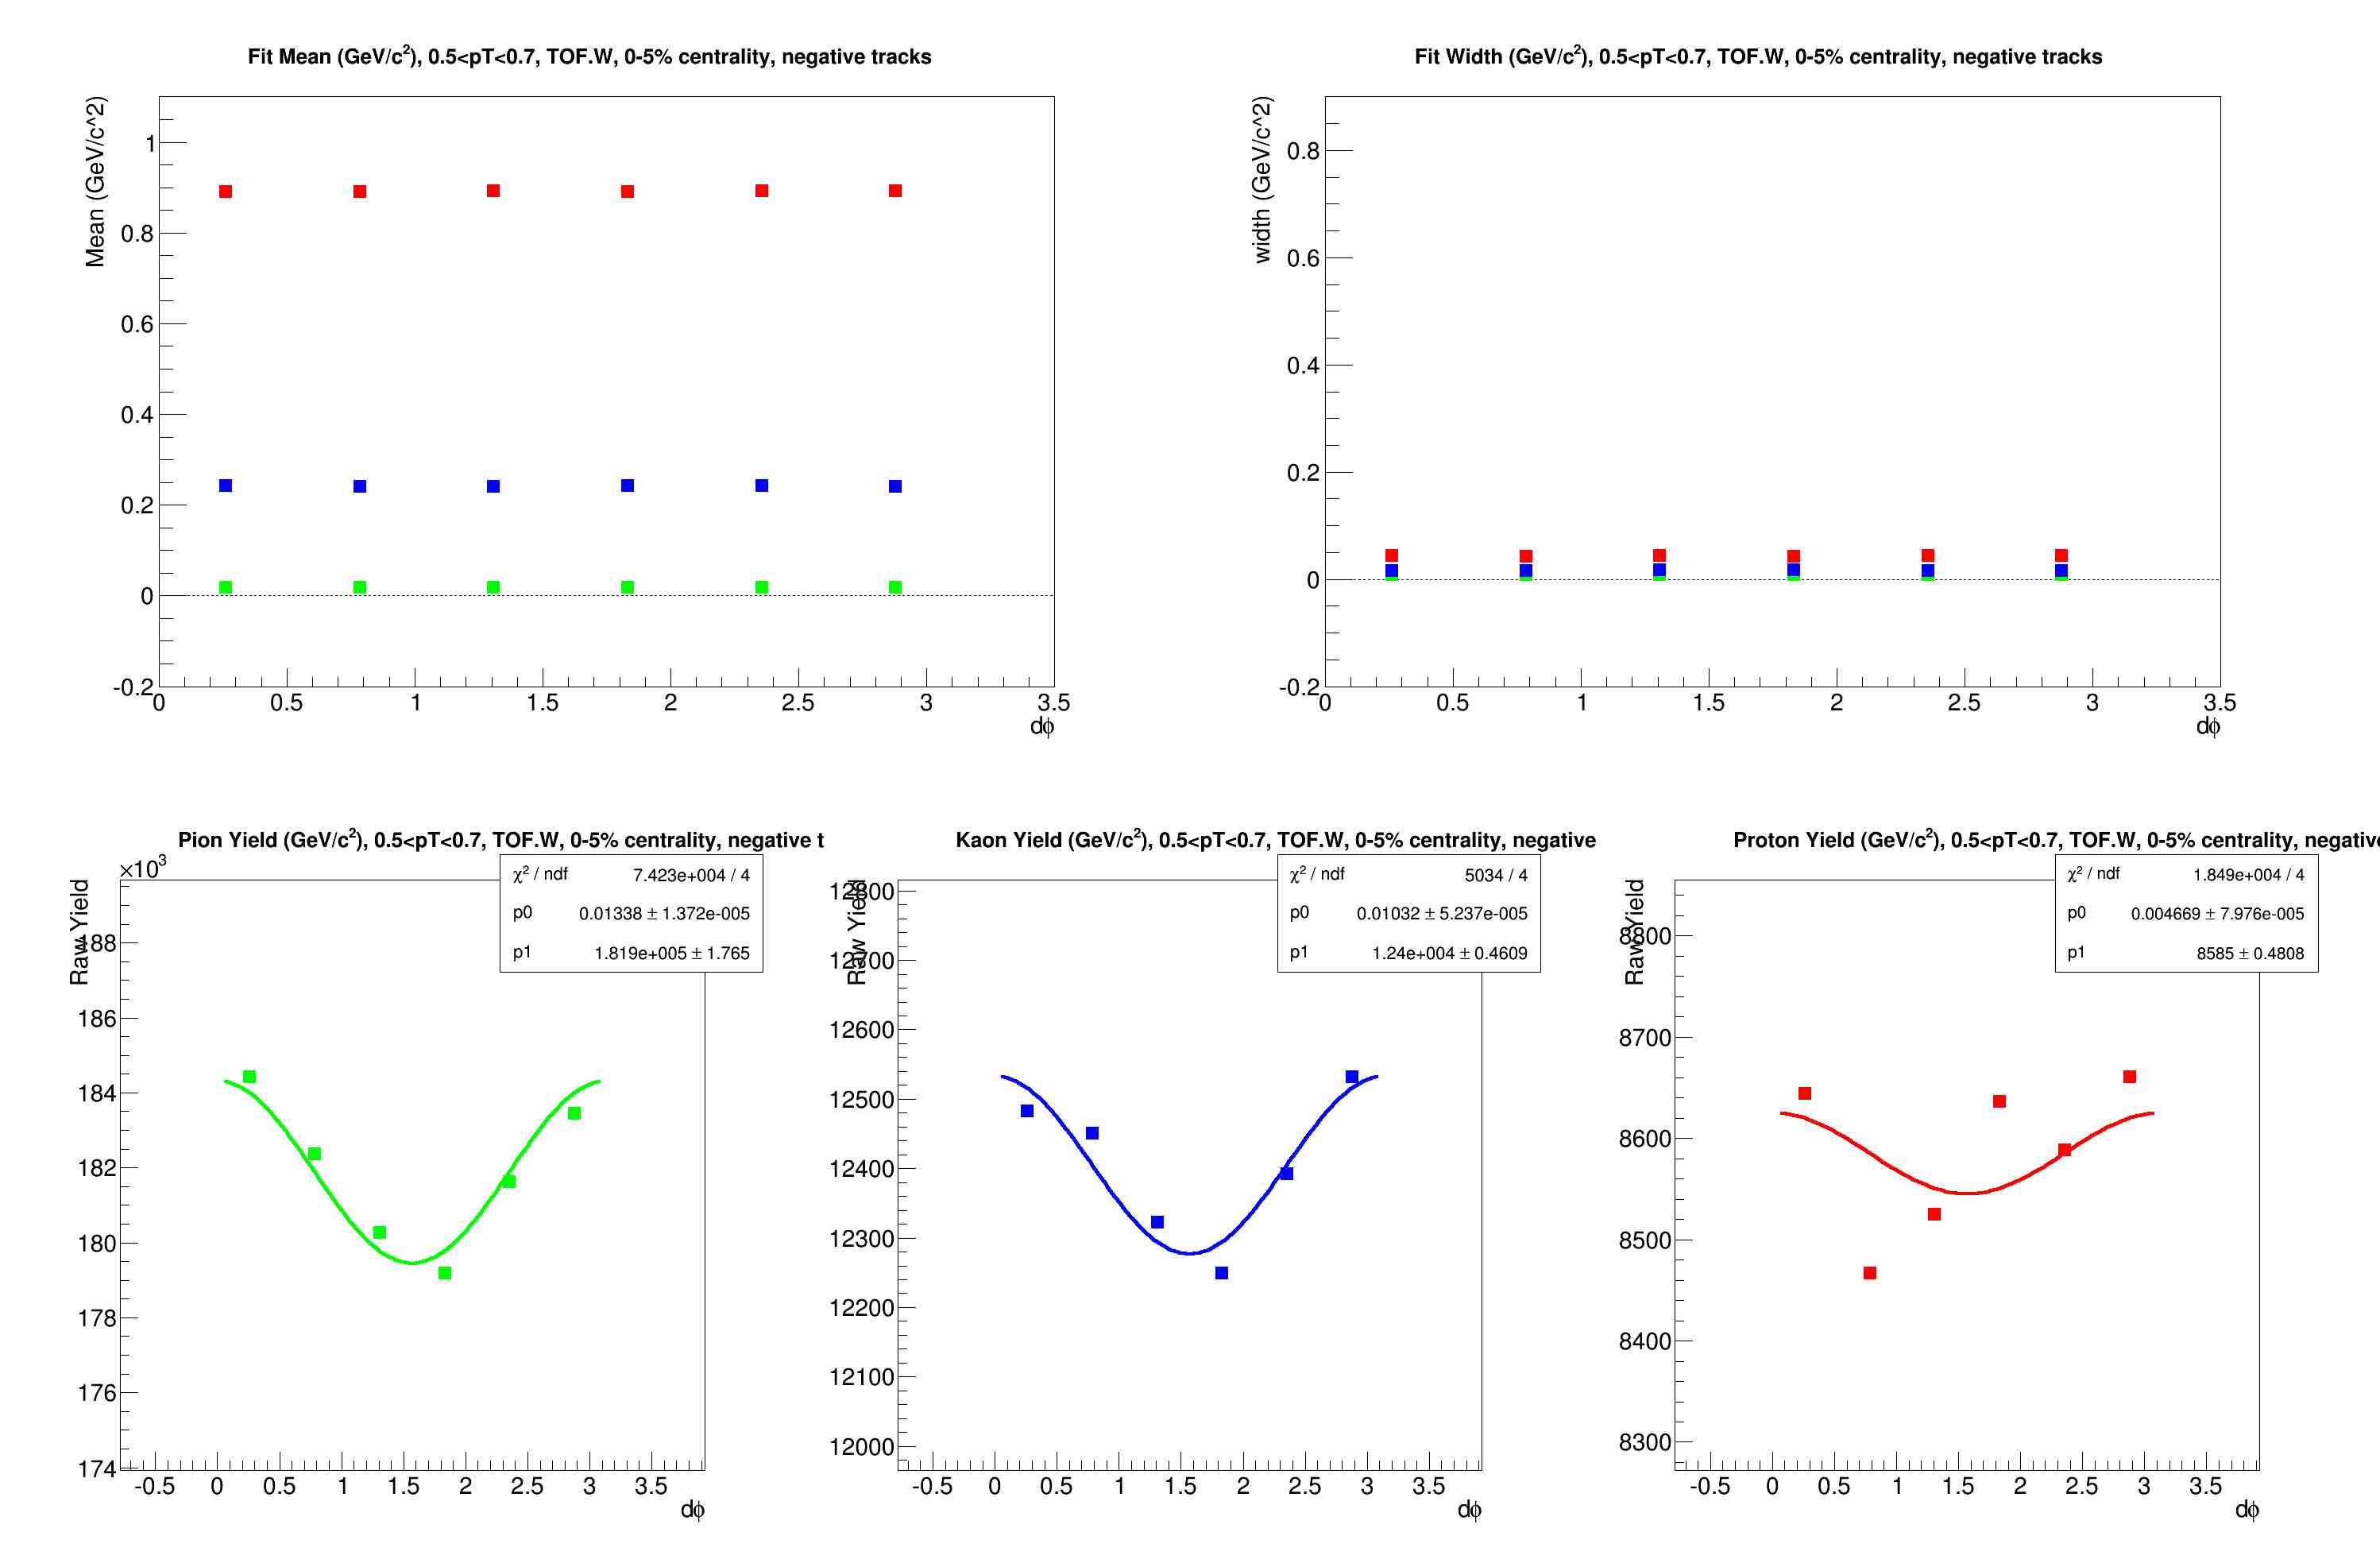
\includegraphics[width=1\textwidth]{lowptfits/fitParams_tof1_cent0_ch0_pT-5-7.jpg}
    \end{subfigure}
    \rule{35em}{0.5pt}
  \caption[PID fits and Yield vs $d\phi$ for $p_T$=0.5-0.7 GeV/c, TOF.W, negative particles ]{$m^2$ Gaussian fits for PID and resulting Yield vs $d\phi$ for $p_T$=0.5-0.7 GeV/c, TOF.W, negative particles}
  \label{fig:fits5-7neg}
\end{figure}

\begin{figure}[H]
  \centering
    \begin{subfigure}{1\textwidth}
    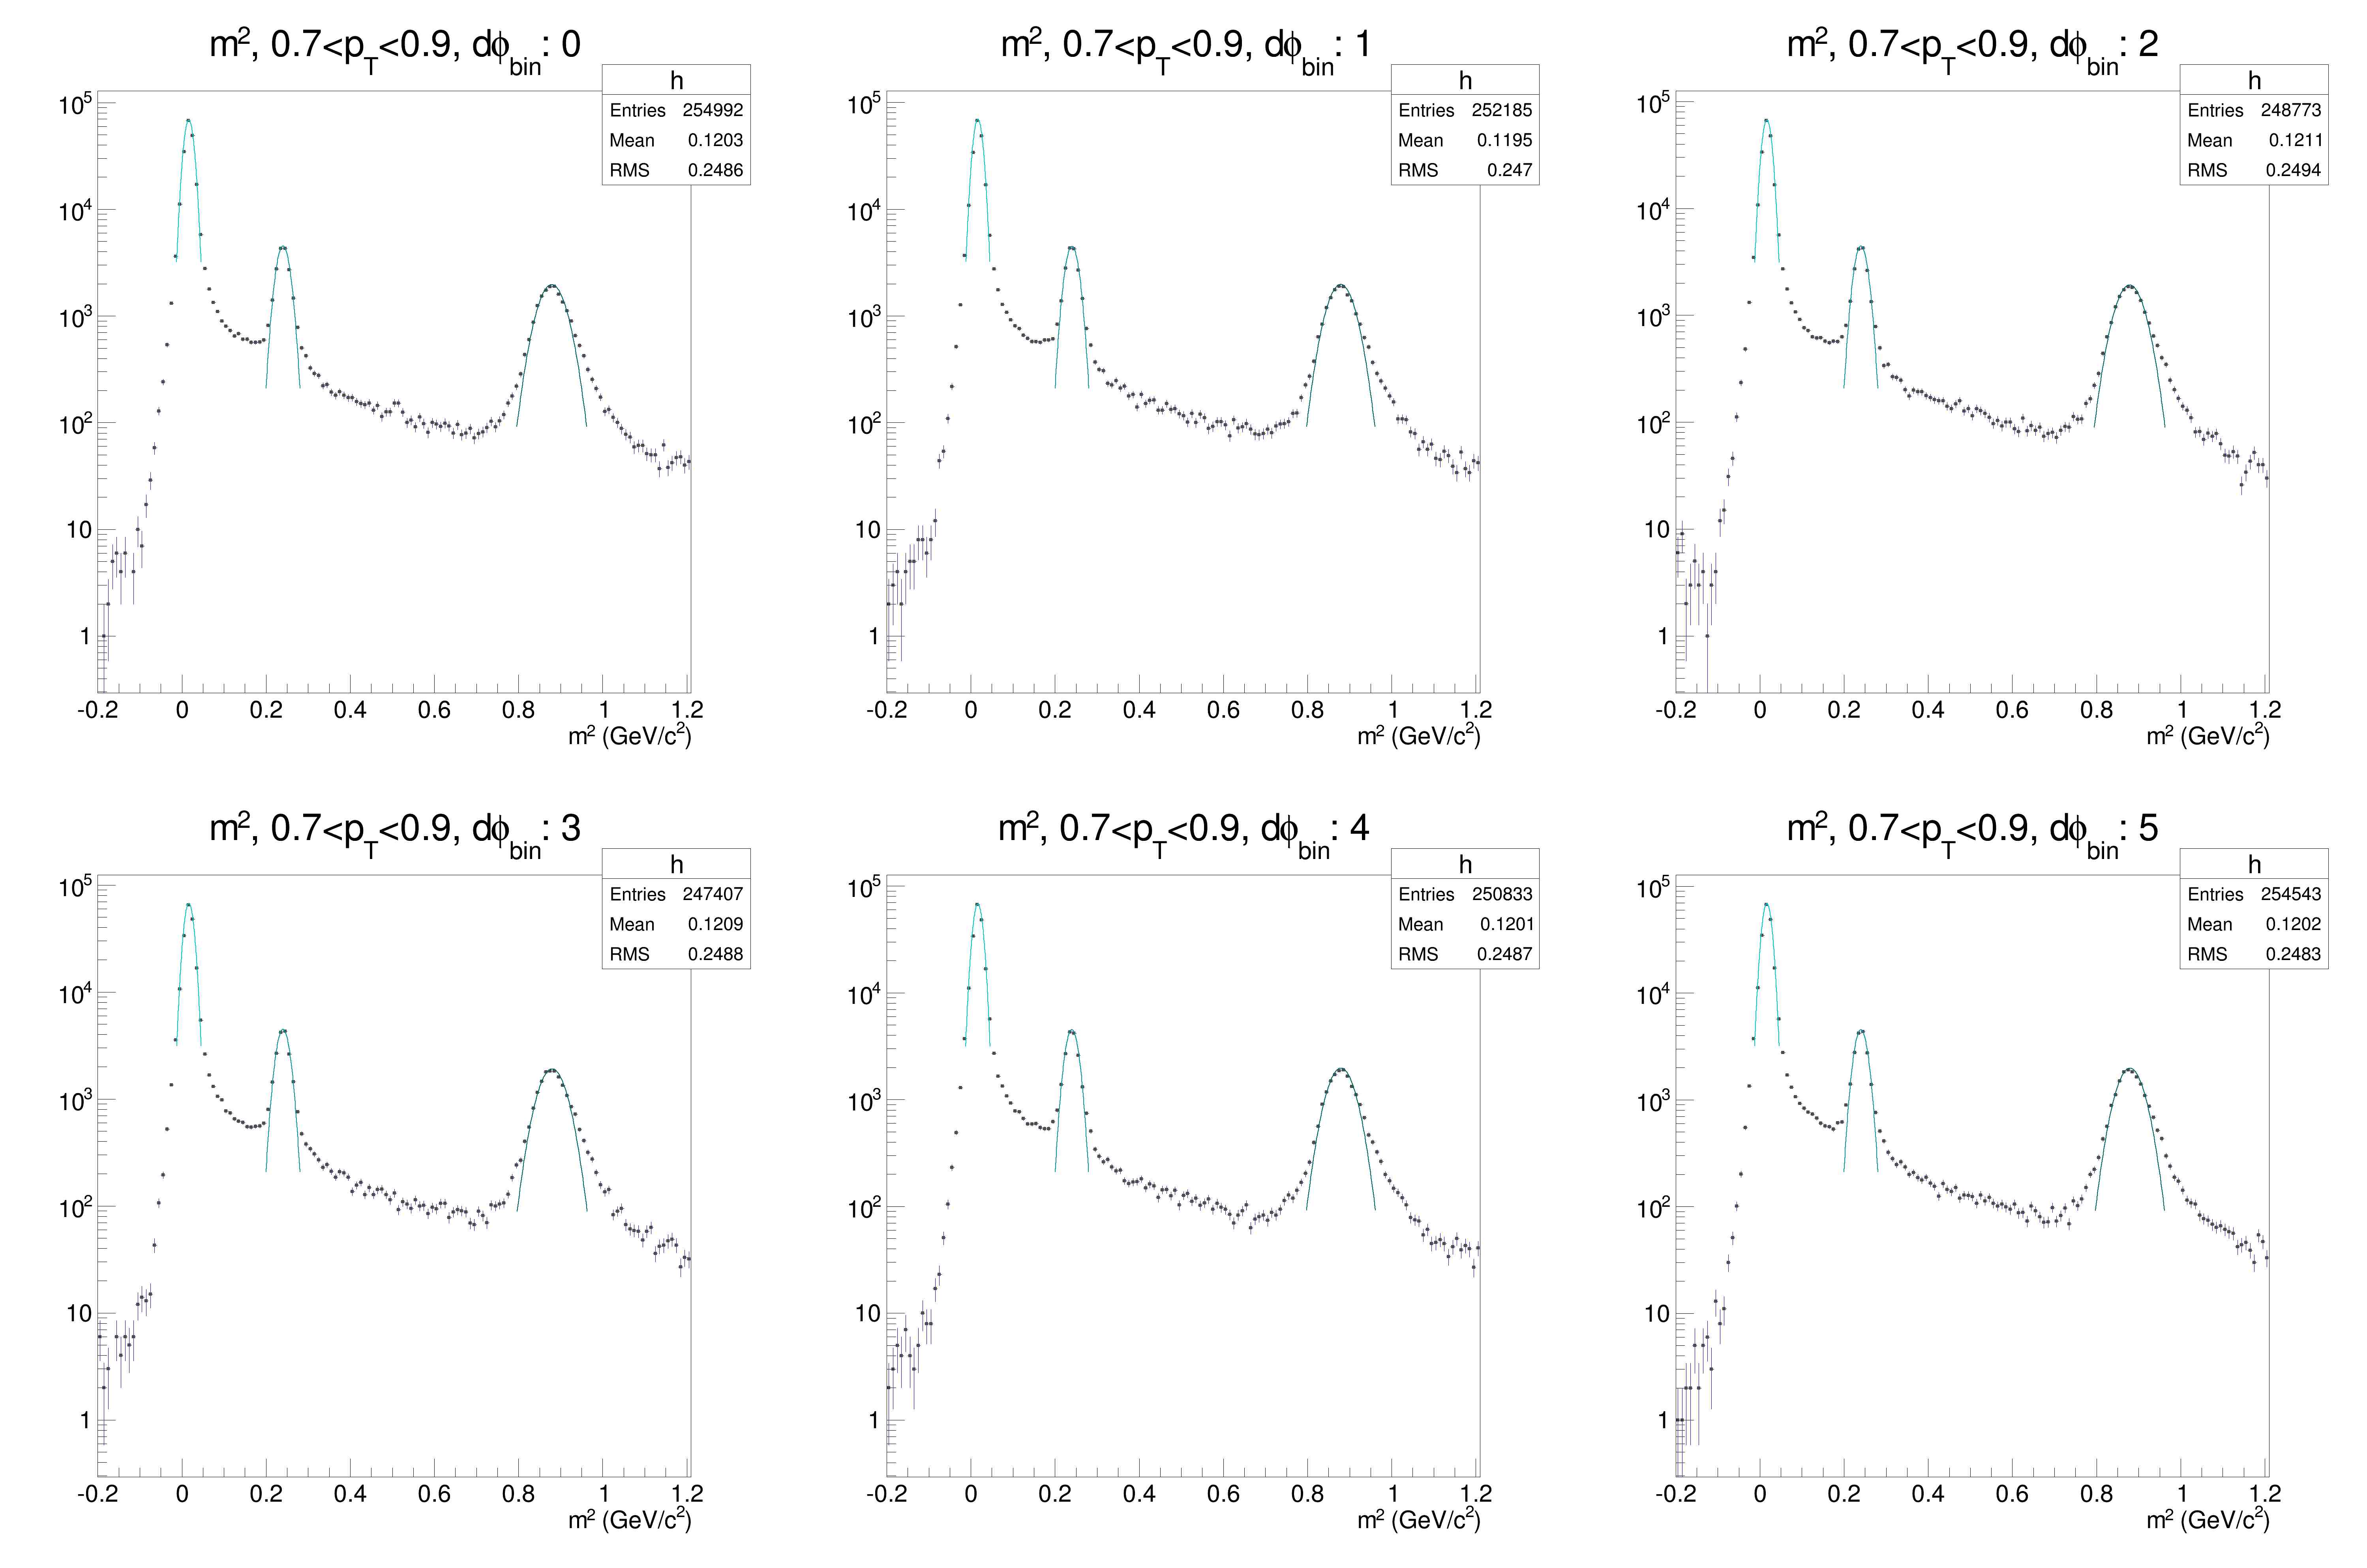
\includegraphics[width=1\textwidth]{lowptfits/yieldvsdphi_tof1_cent0_ch0_pT-7-9.jpg}
    \end{subfigure}
    \begin{subfigure}{1\textwidth}
    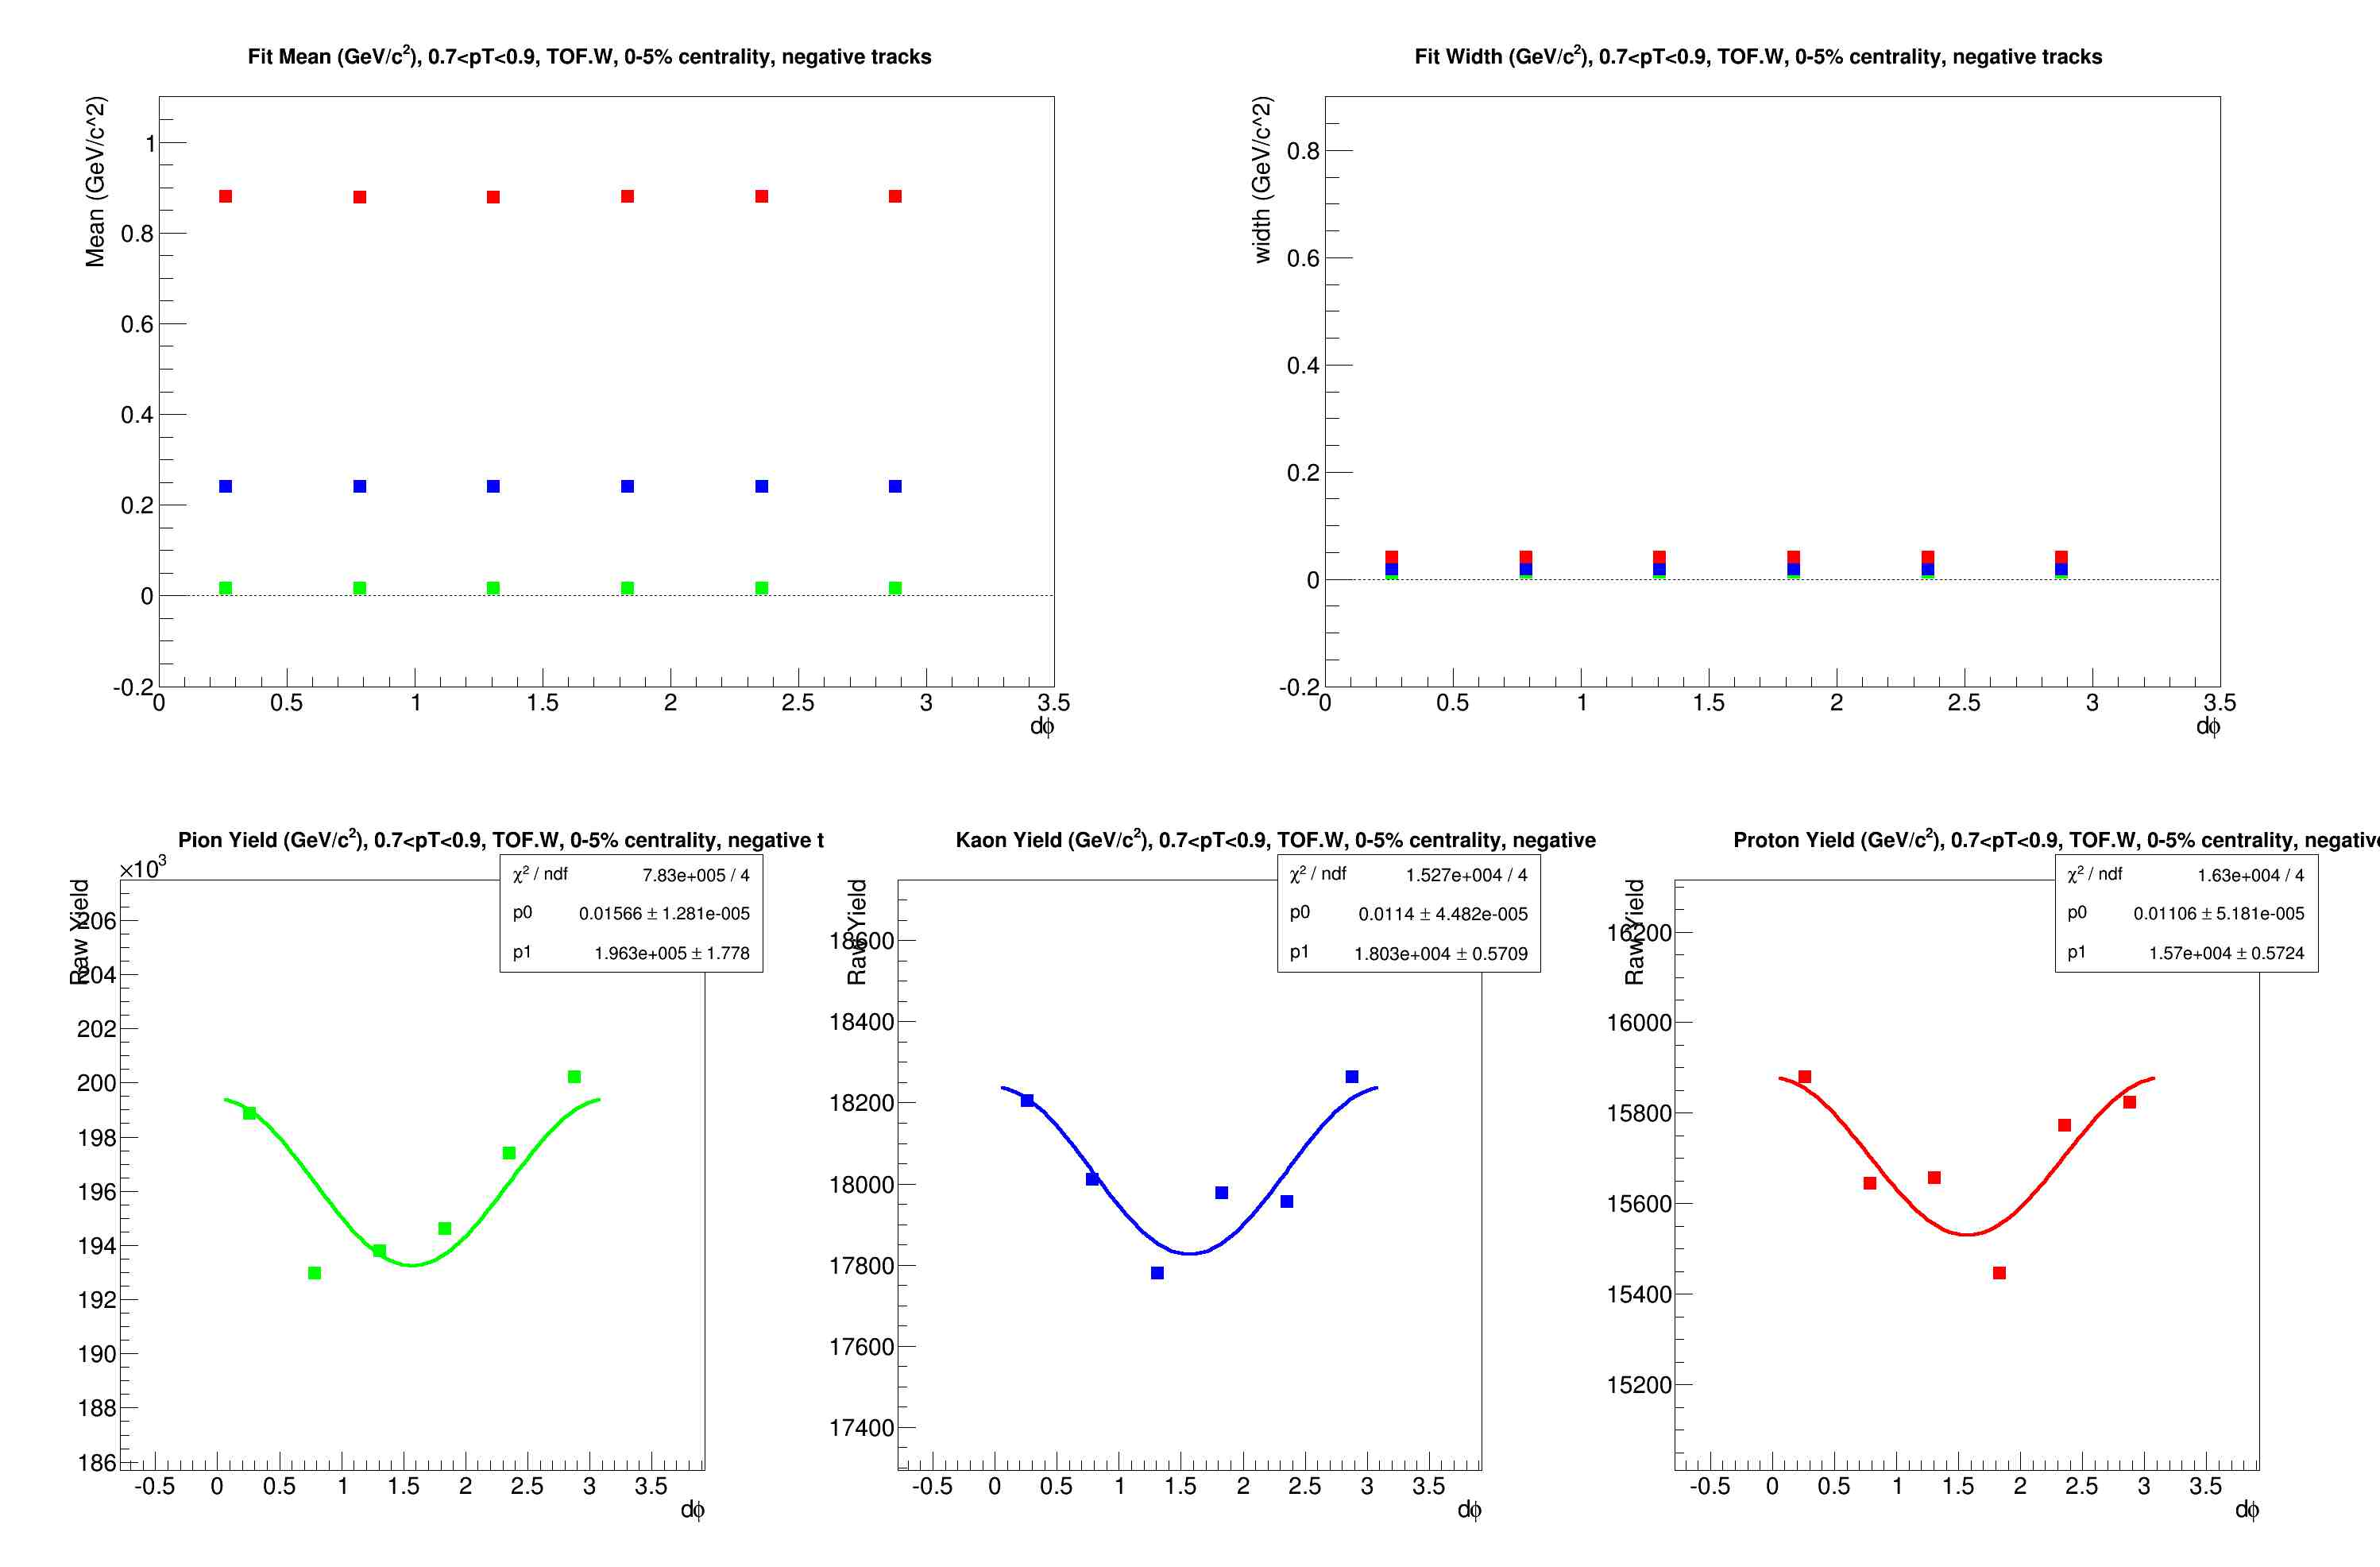
\includegraphics[width=1\textwidth]{lowptfits/fitParams_tof1_cent0_ch0_pT-7-9.jpg}
    \end{subfigure}
    \rule{35em}{0.5pt}
  \caption[PID fits and Yield vs $d\phi$ for $p_T$=0.7-0.9 GeV/c, TOF.W, negative particles ]{$m^2$ Gaussian fits for PID and resulting Yield vs $d\phi$ for $p_T$=0.7-0.9 GeV/c, TOF.W, negative particles}
  \label{fig:fits7-9neg}
\end{figure}

\begin{figure}[H]
  \centering
    \begin{subfigure}[p]{1\textwidth}
    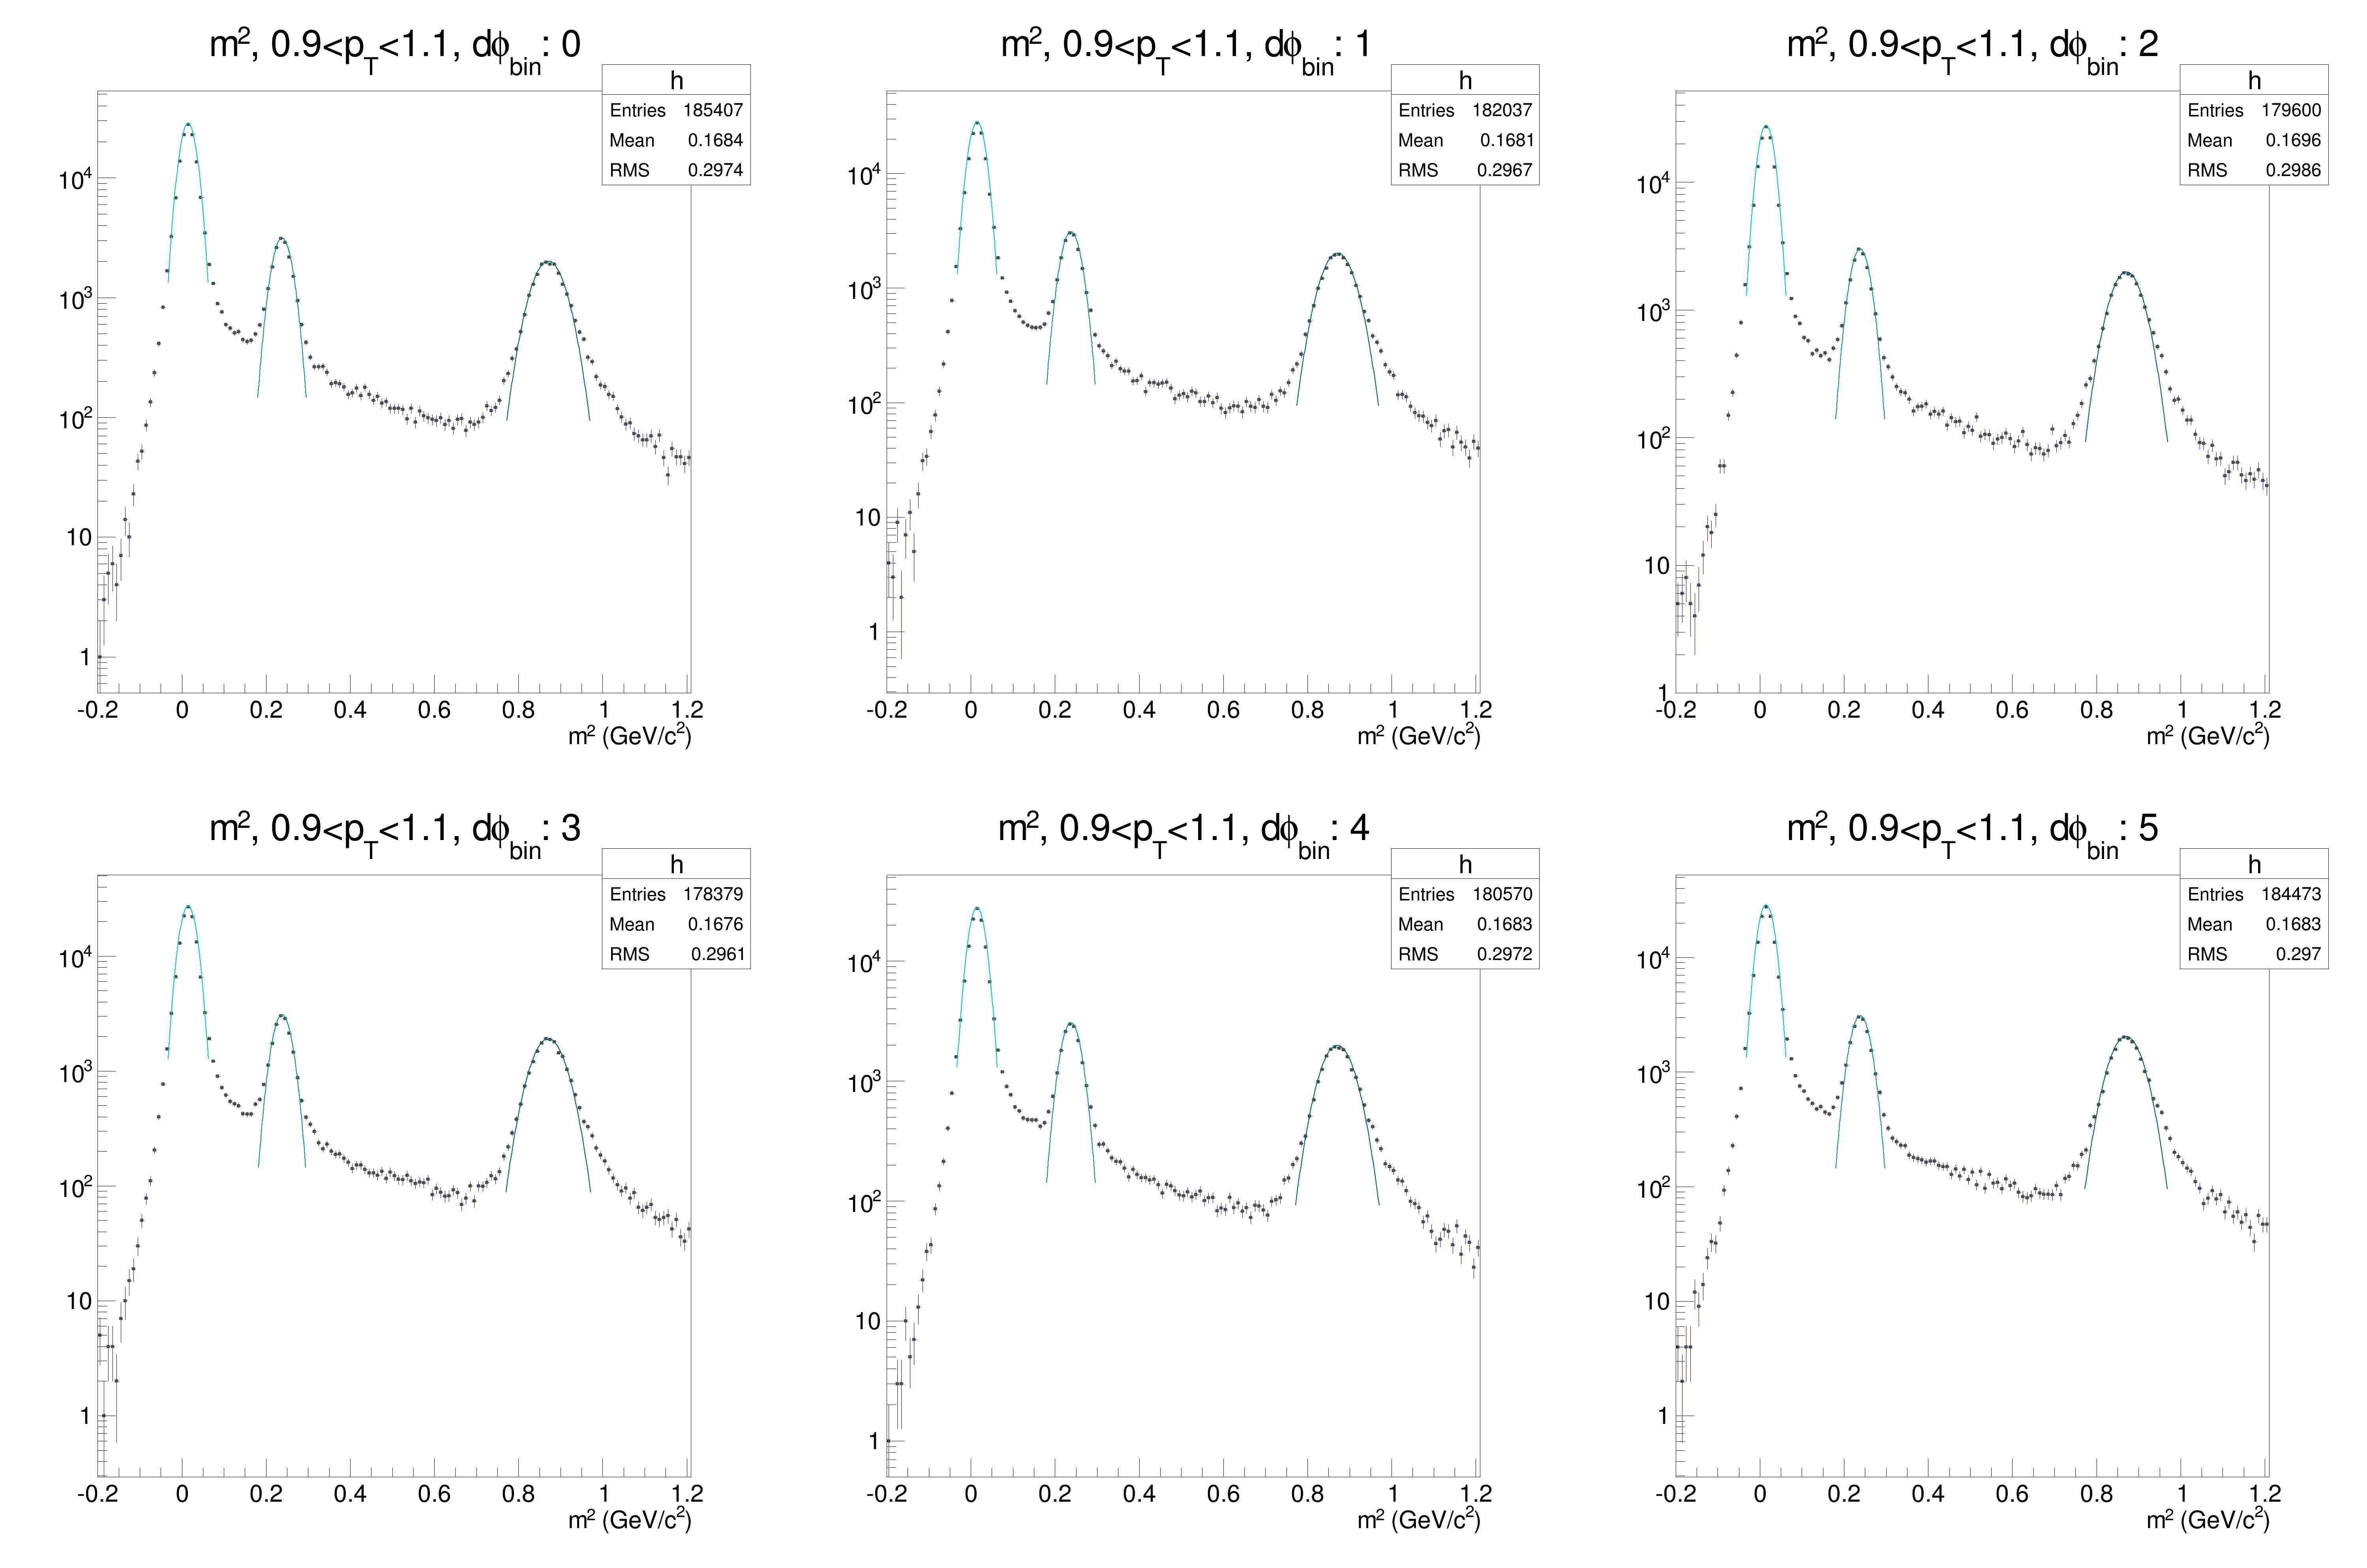
\includegraphics[width=1\textwidth]{lowptfits/yieldvsdphi_tof1_cent0_ch0_pT-9-11.jpg}
    \end{subfigure}
    \begin{subfigure}[p]{1\textwidth}
    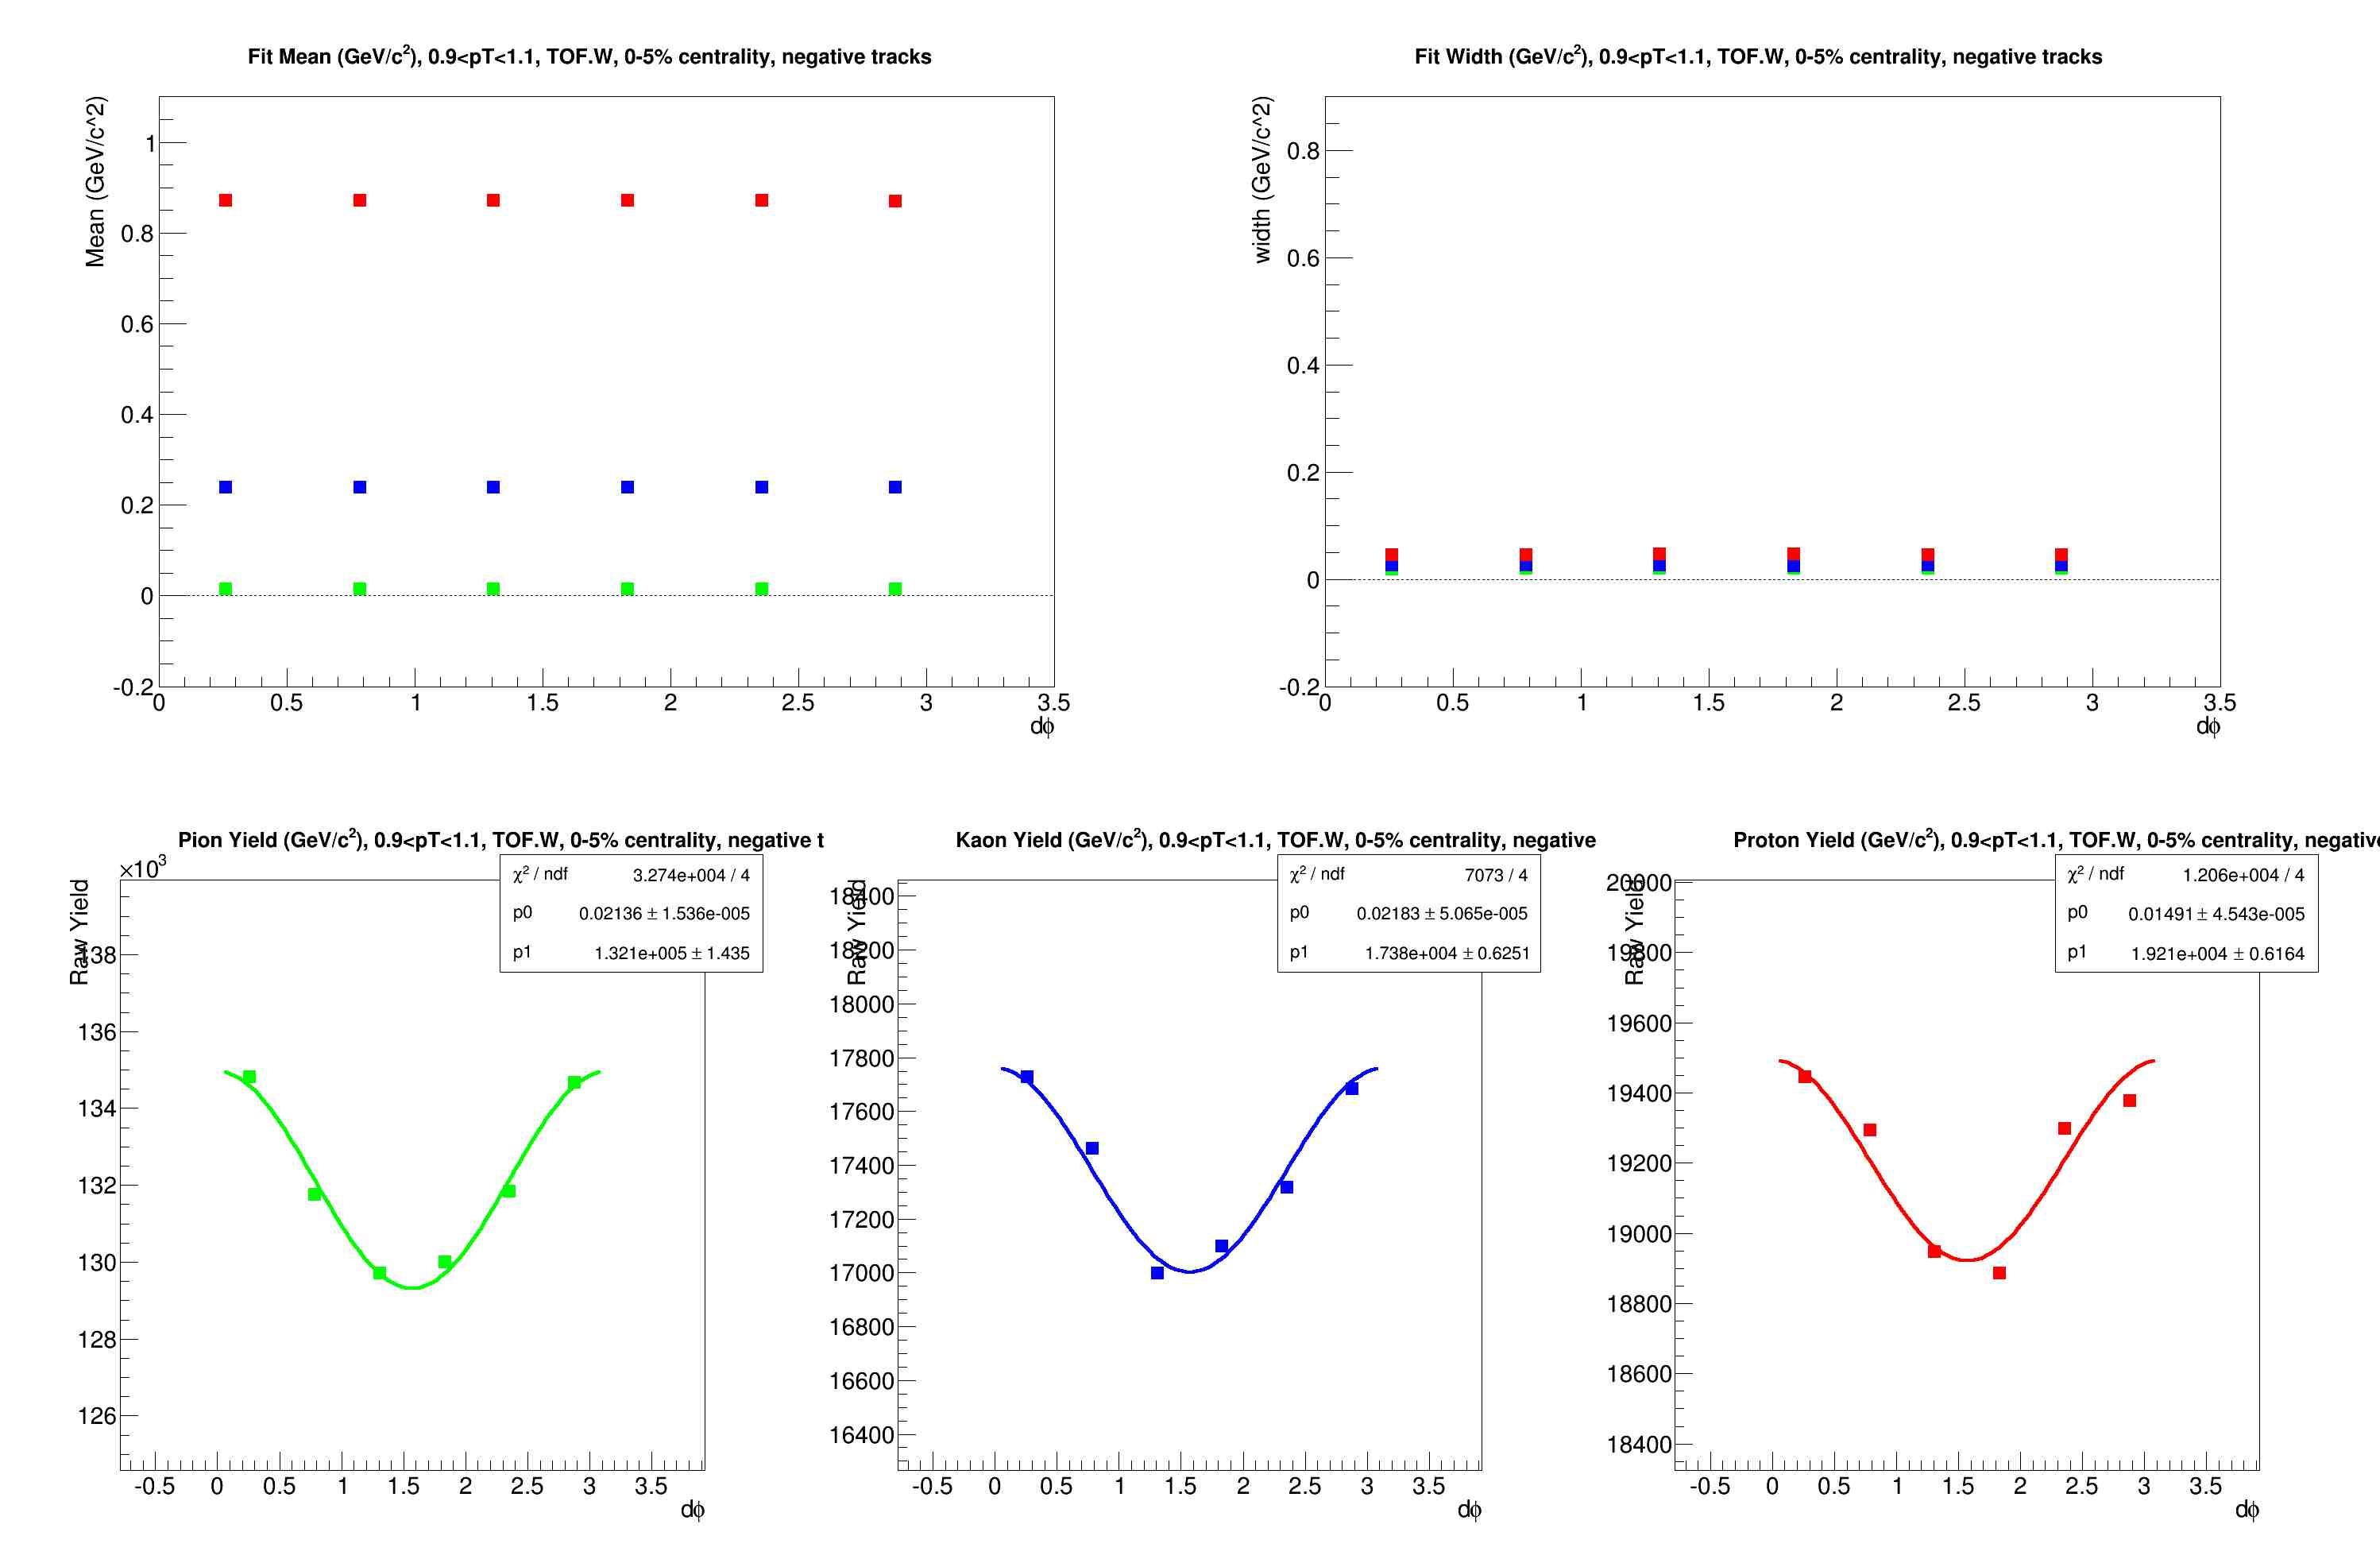
\includegraphics[width=1\textwidth]{lowptfits/fitParams_tof1_cent0_ch0_pT-9-11.jpg}
    \end{subfigure}
    \rule{35em}{0.5pt}
  \caption[PID fits and Yield vs $d\phi$ for $p_T$=0.9-1.1 GeV/c, TOF.W, negative particles ]{$m^2$ Gaussian fits for PID and resulting Yield vs $d\phi$ for $p_T$=0.9-1.1 GeV/c, TOF.W, negative particles}
  \label{fig:fits9-11neg}
\end{figure}

\begin{figure}[H]
  \centering
    \begin{subfigure}[p]{1\textwidth}
    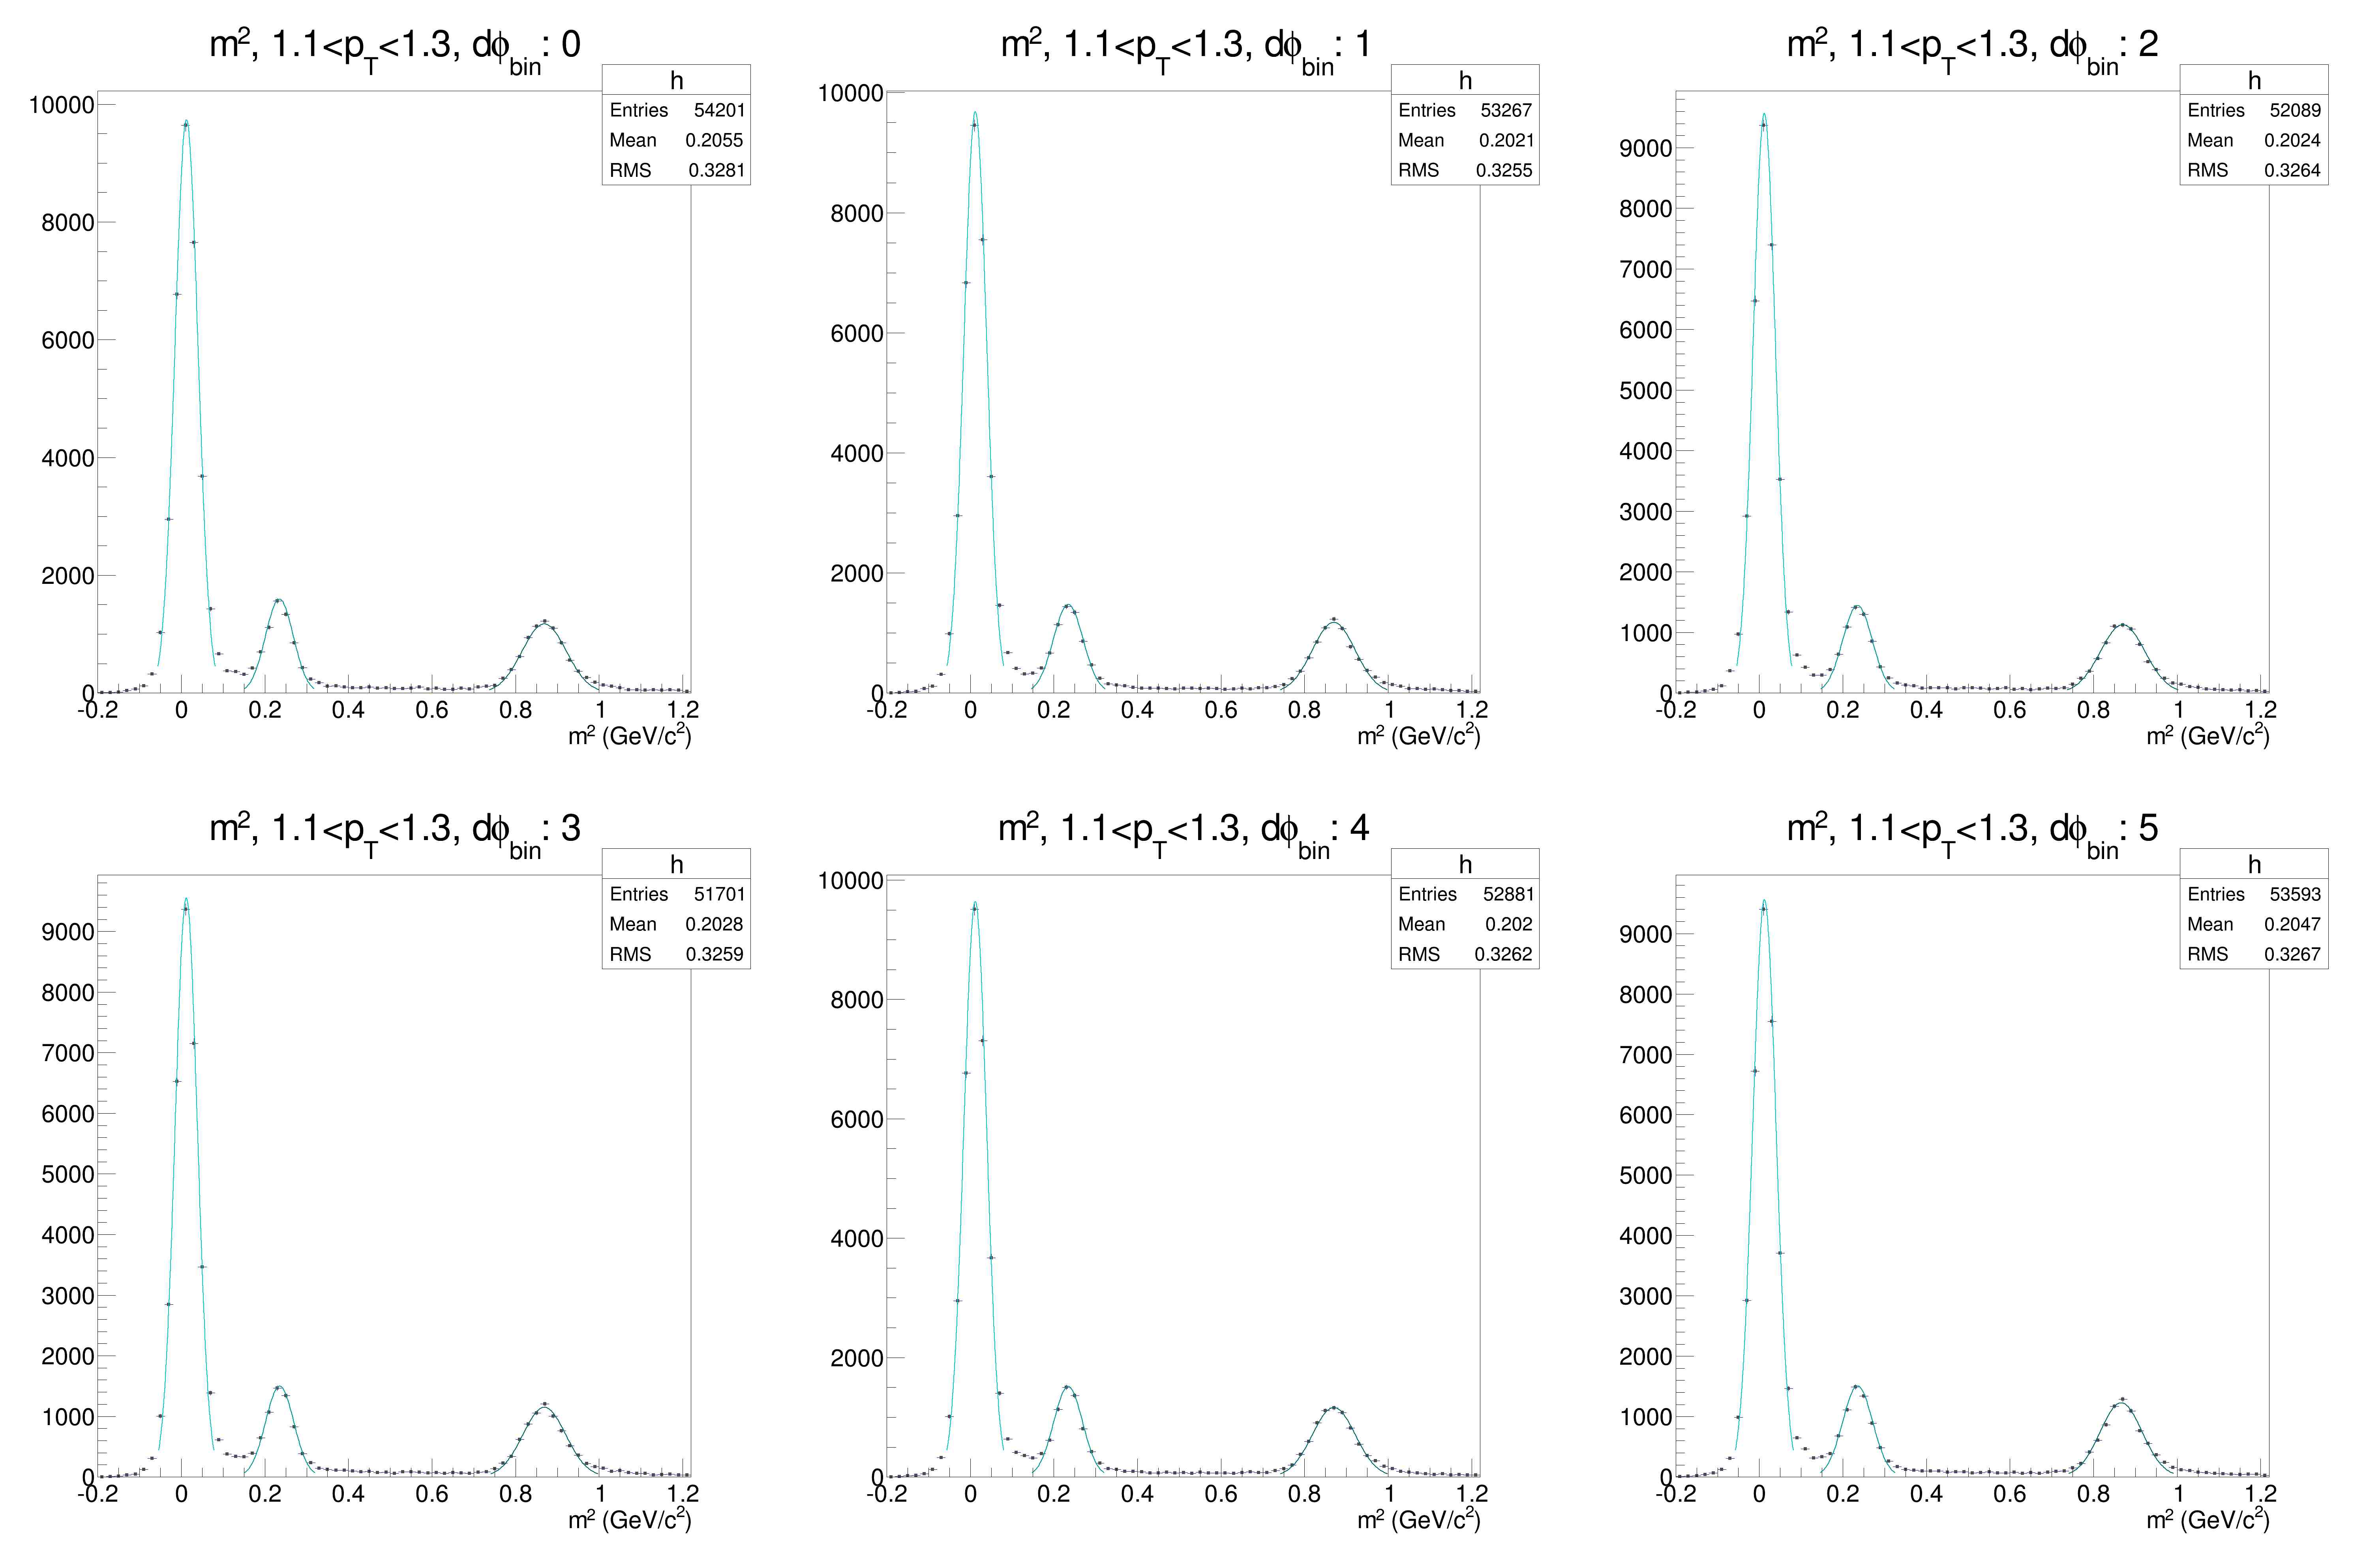
\includegraphics[width=1\textwidth]{lowptfits/yieldvsdphi_tof1_cent0_ch0_pT-11-13.jpg}
    \end{subfigure}
    \begin{subfigure}[p]{1\textwidth}
    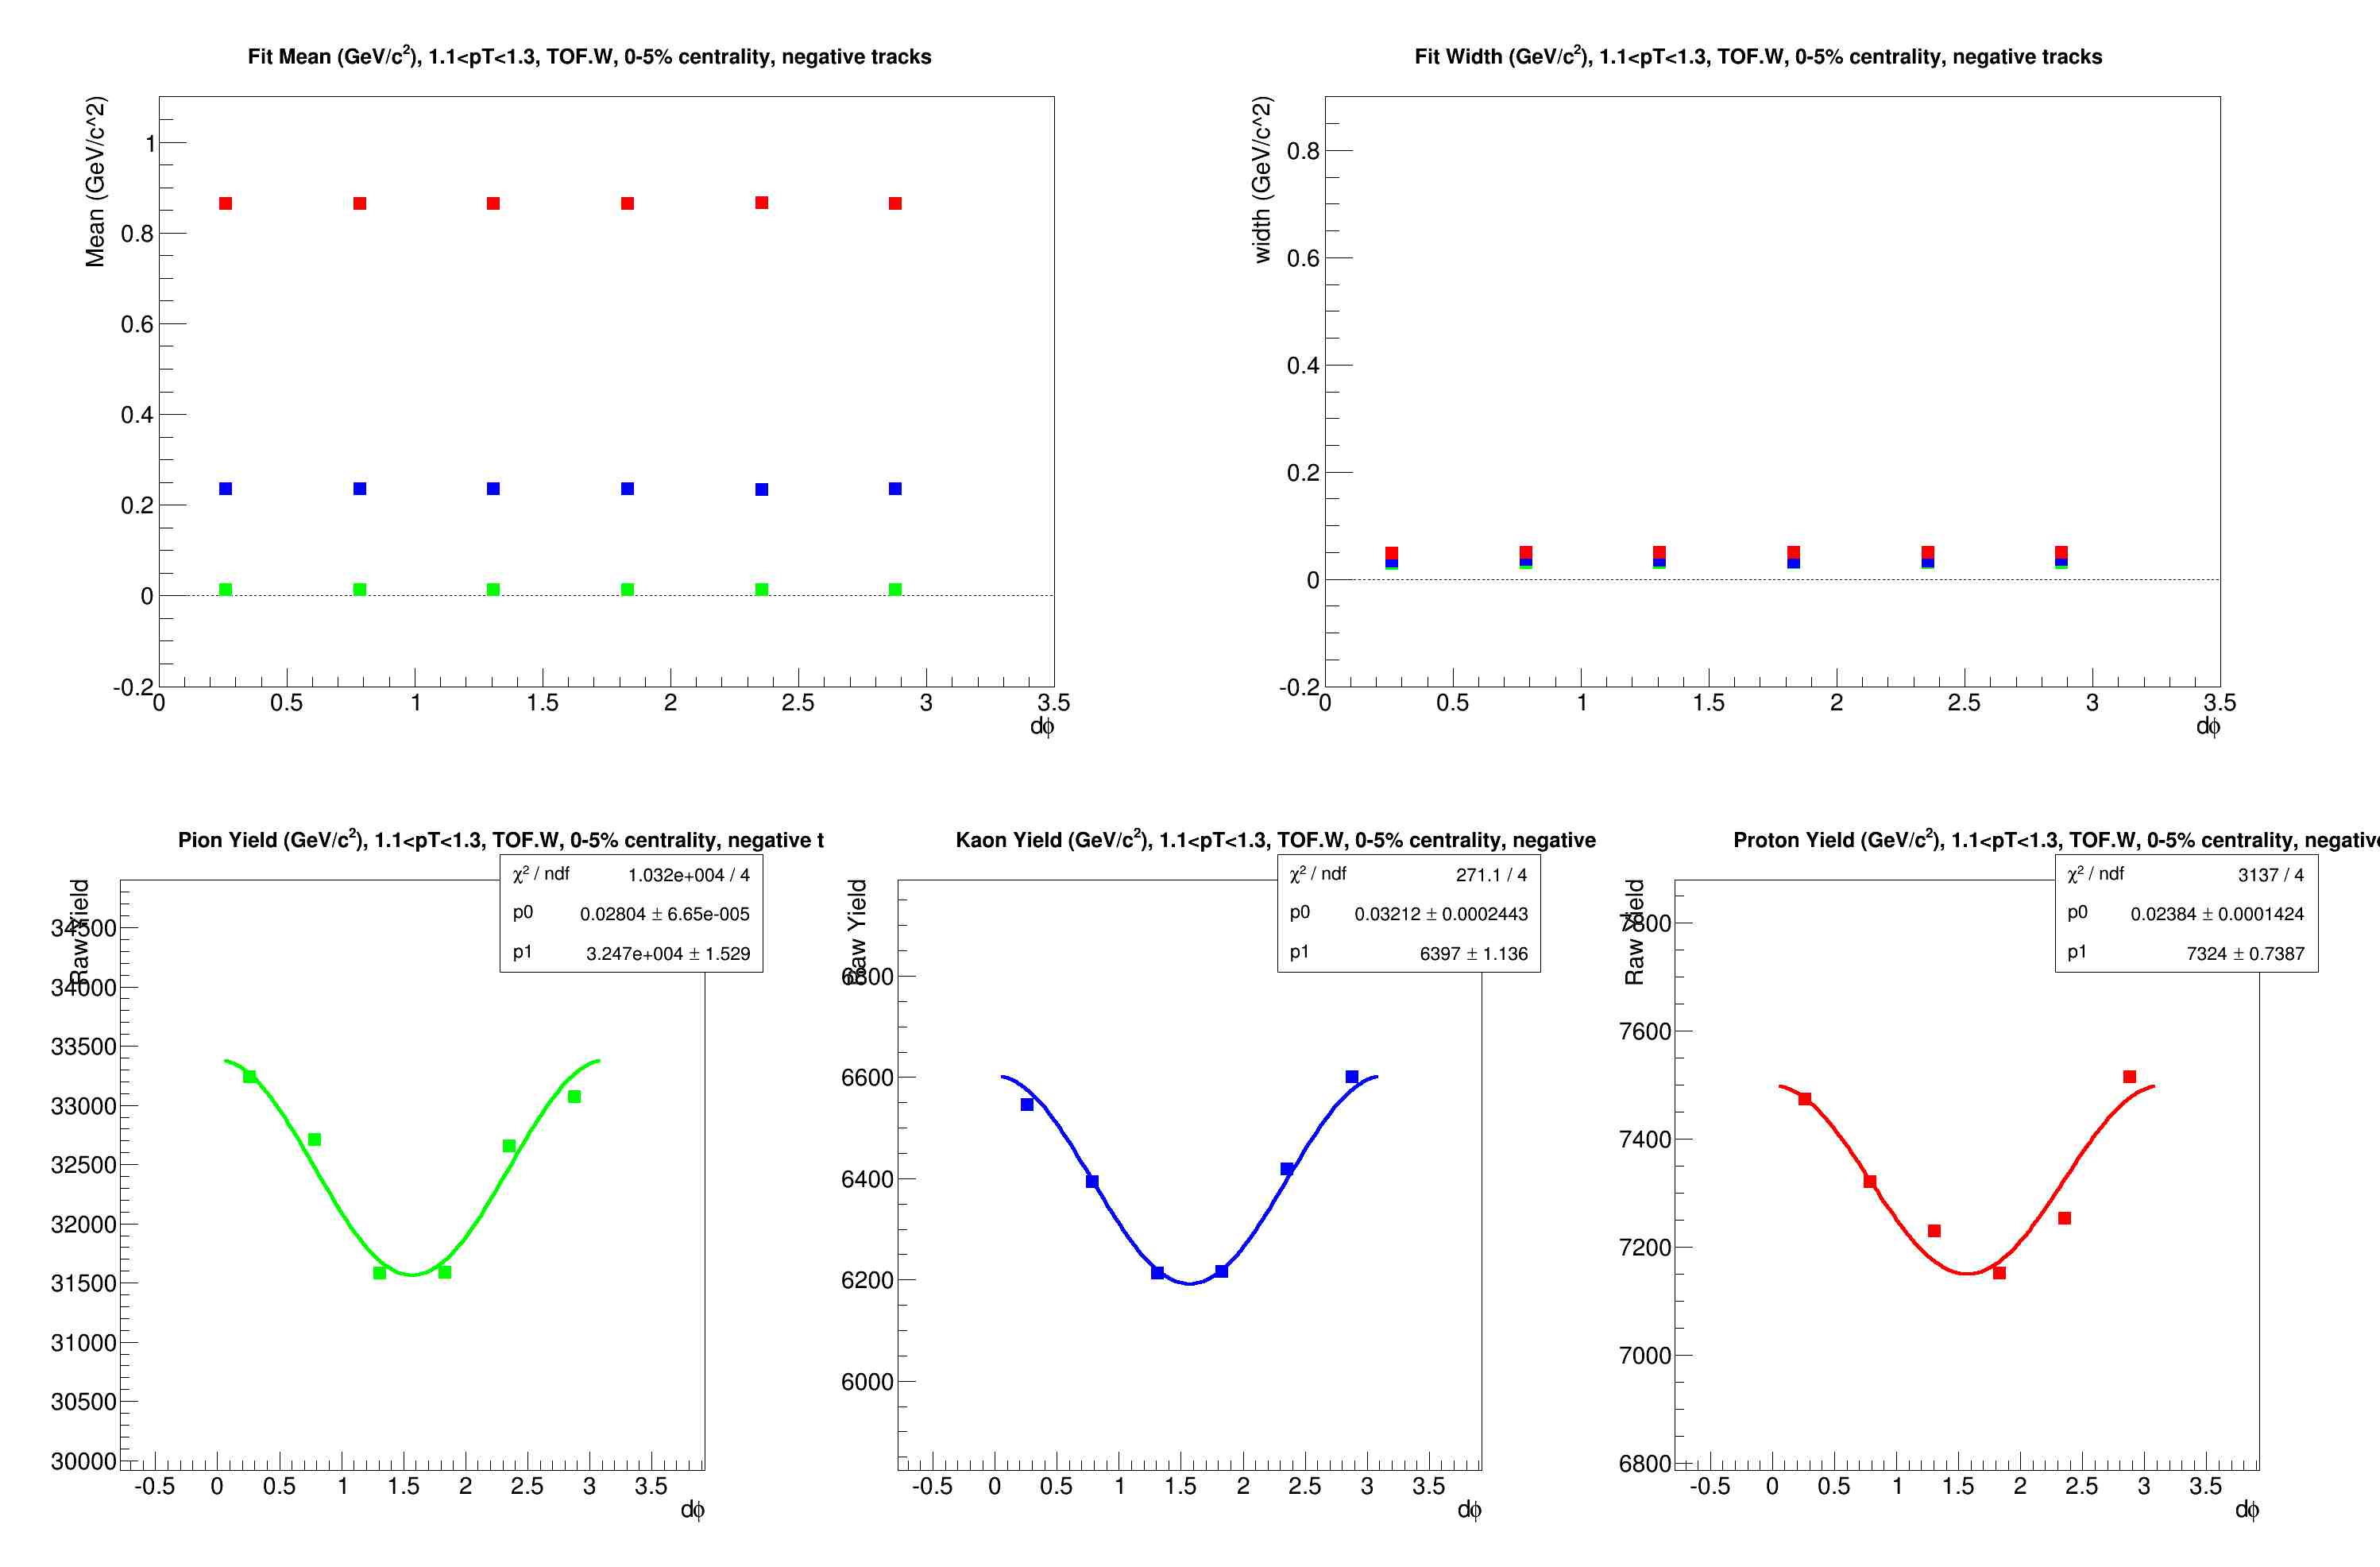
\includegraphics[width=1\textwidth]{lowptfits/fitParams_tof1_cent0_ch0_pT-11-13.jpg}
    \end{subfigure}
    \rule{35em}{0.5pt}
  \caption[PID fits and Yield vs $d\phi$ for $p_T$=1.1-1.3 GeV/c, TOF.W, negative particles ]{$m^2$ Gaussian fits for PID and resulting Yield vs $d\phi$ for $p_T$=1.1-1.3 GeV/c, TOF.W, negative particles}
  \label{fig:fits11-13neg}
\end{figure}

\subsubsection{Single Gaussian fits, $p_T$=0.5-1.3 GeV/c, TOF.W, positive charged tracks}

\begin{figure}[H]
  \centering
    \begin{subfigure}[p]{1\textwidth}
    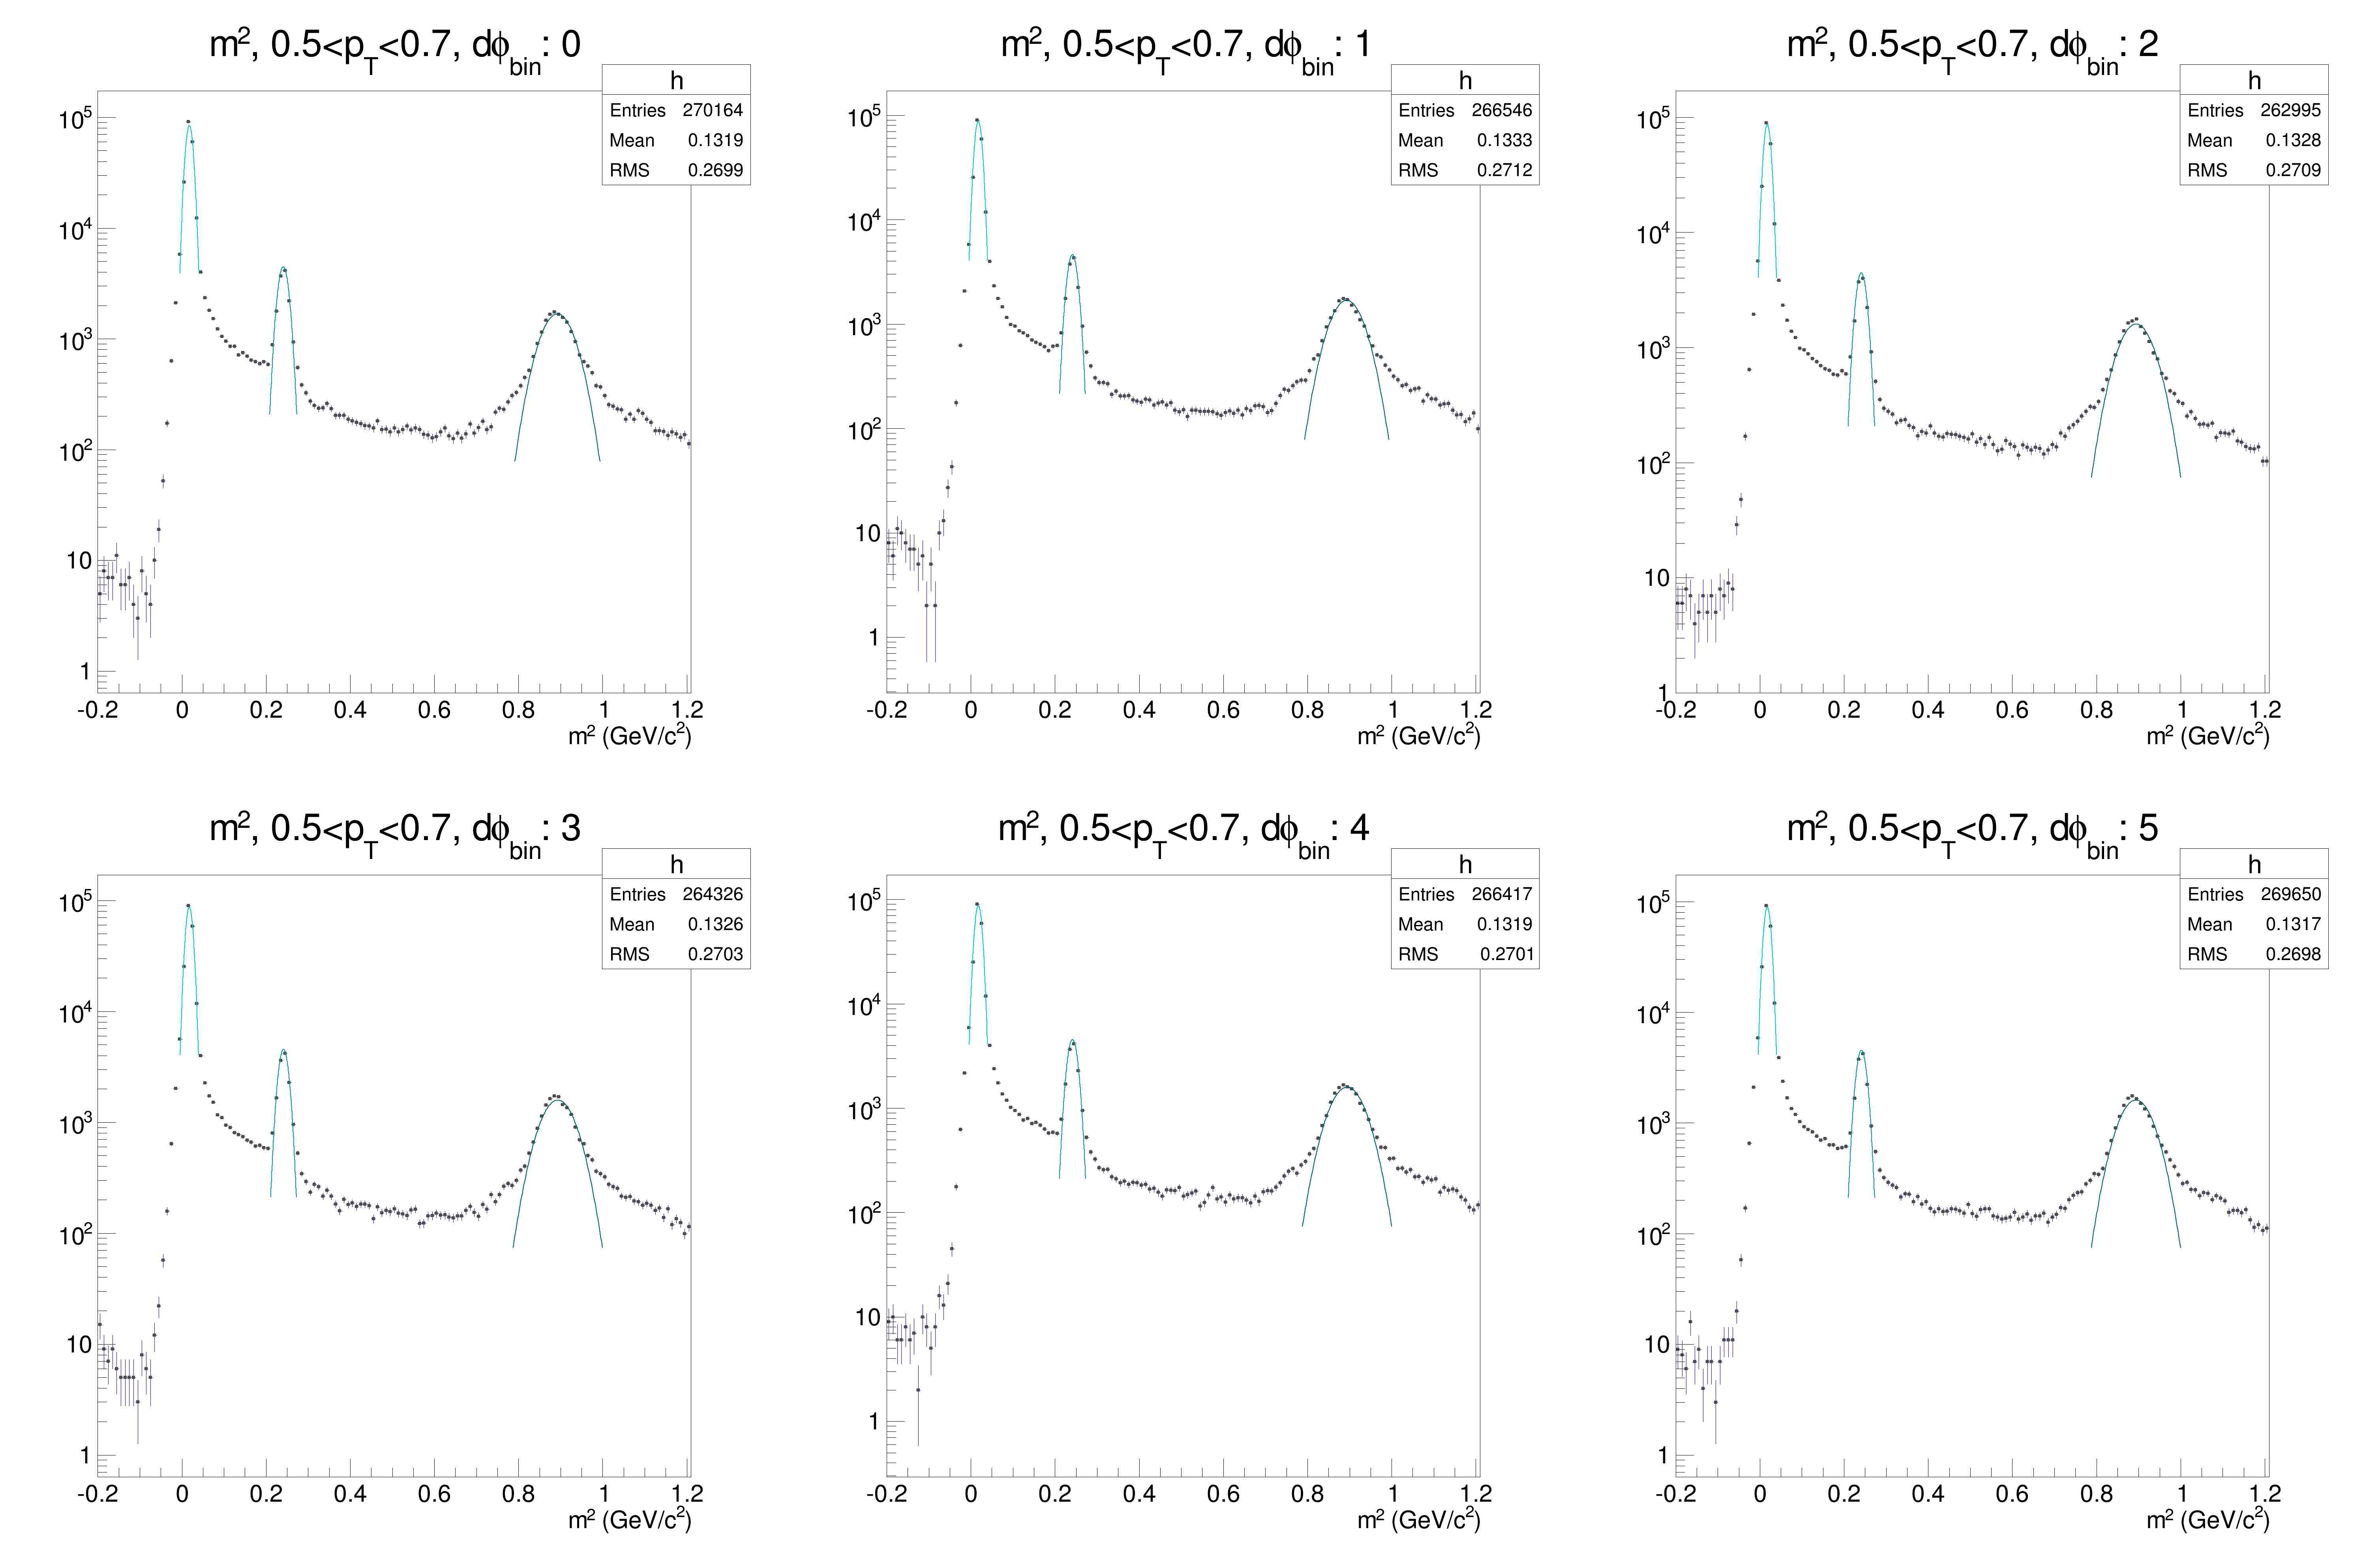
\includegraphics[width=1\textwidth]{lowptfits/yieldvsdphi_tof1_cent0_ch1_pT-5-7.jpg}
    \end{subfigure}
    \begin{subfigure}[p]{1\textwidth}
    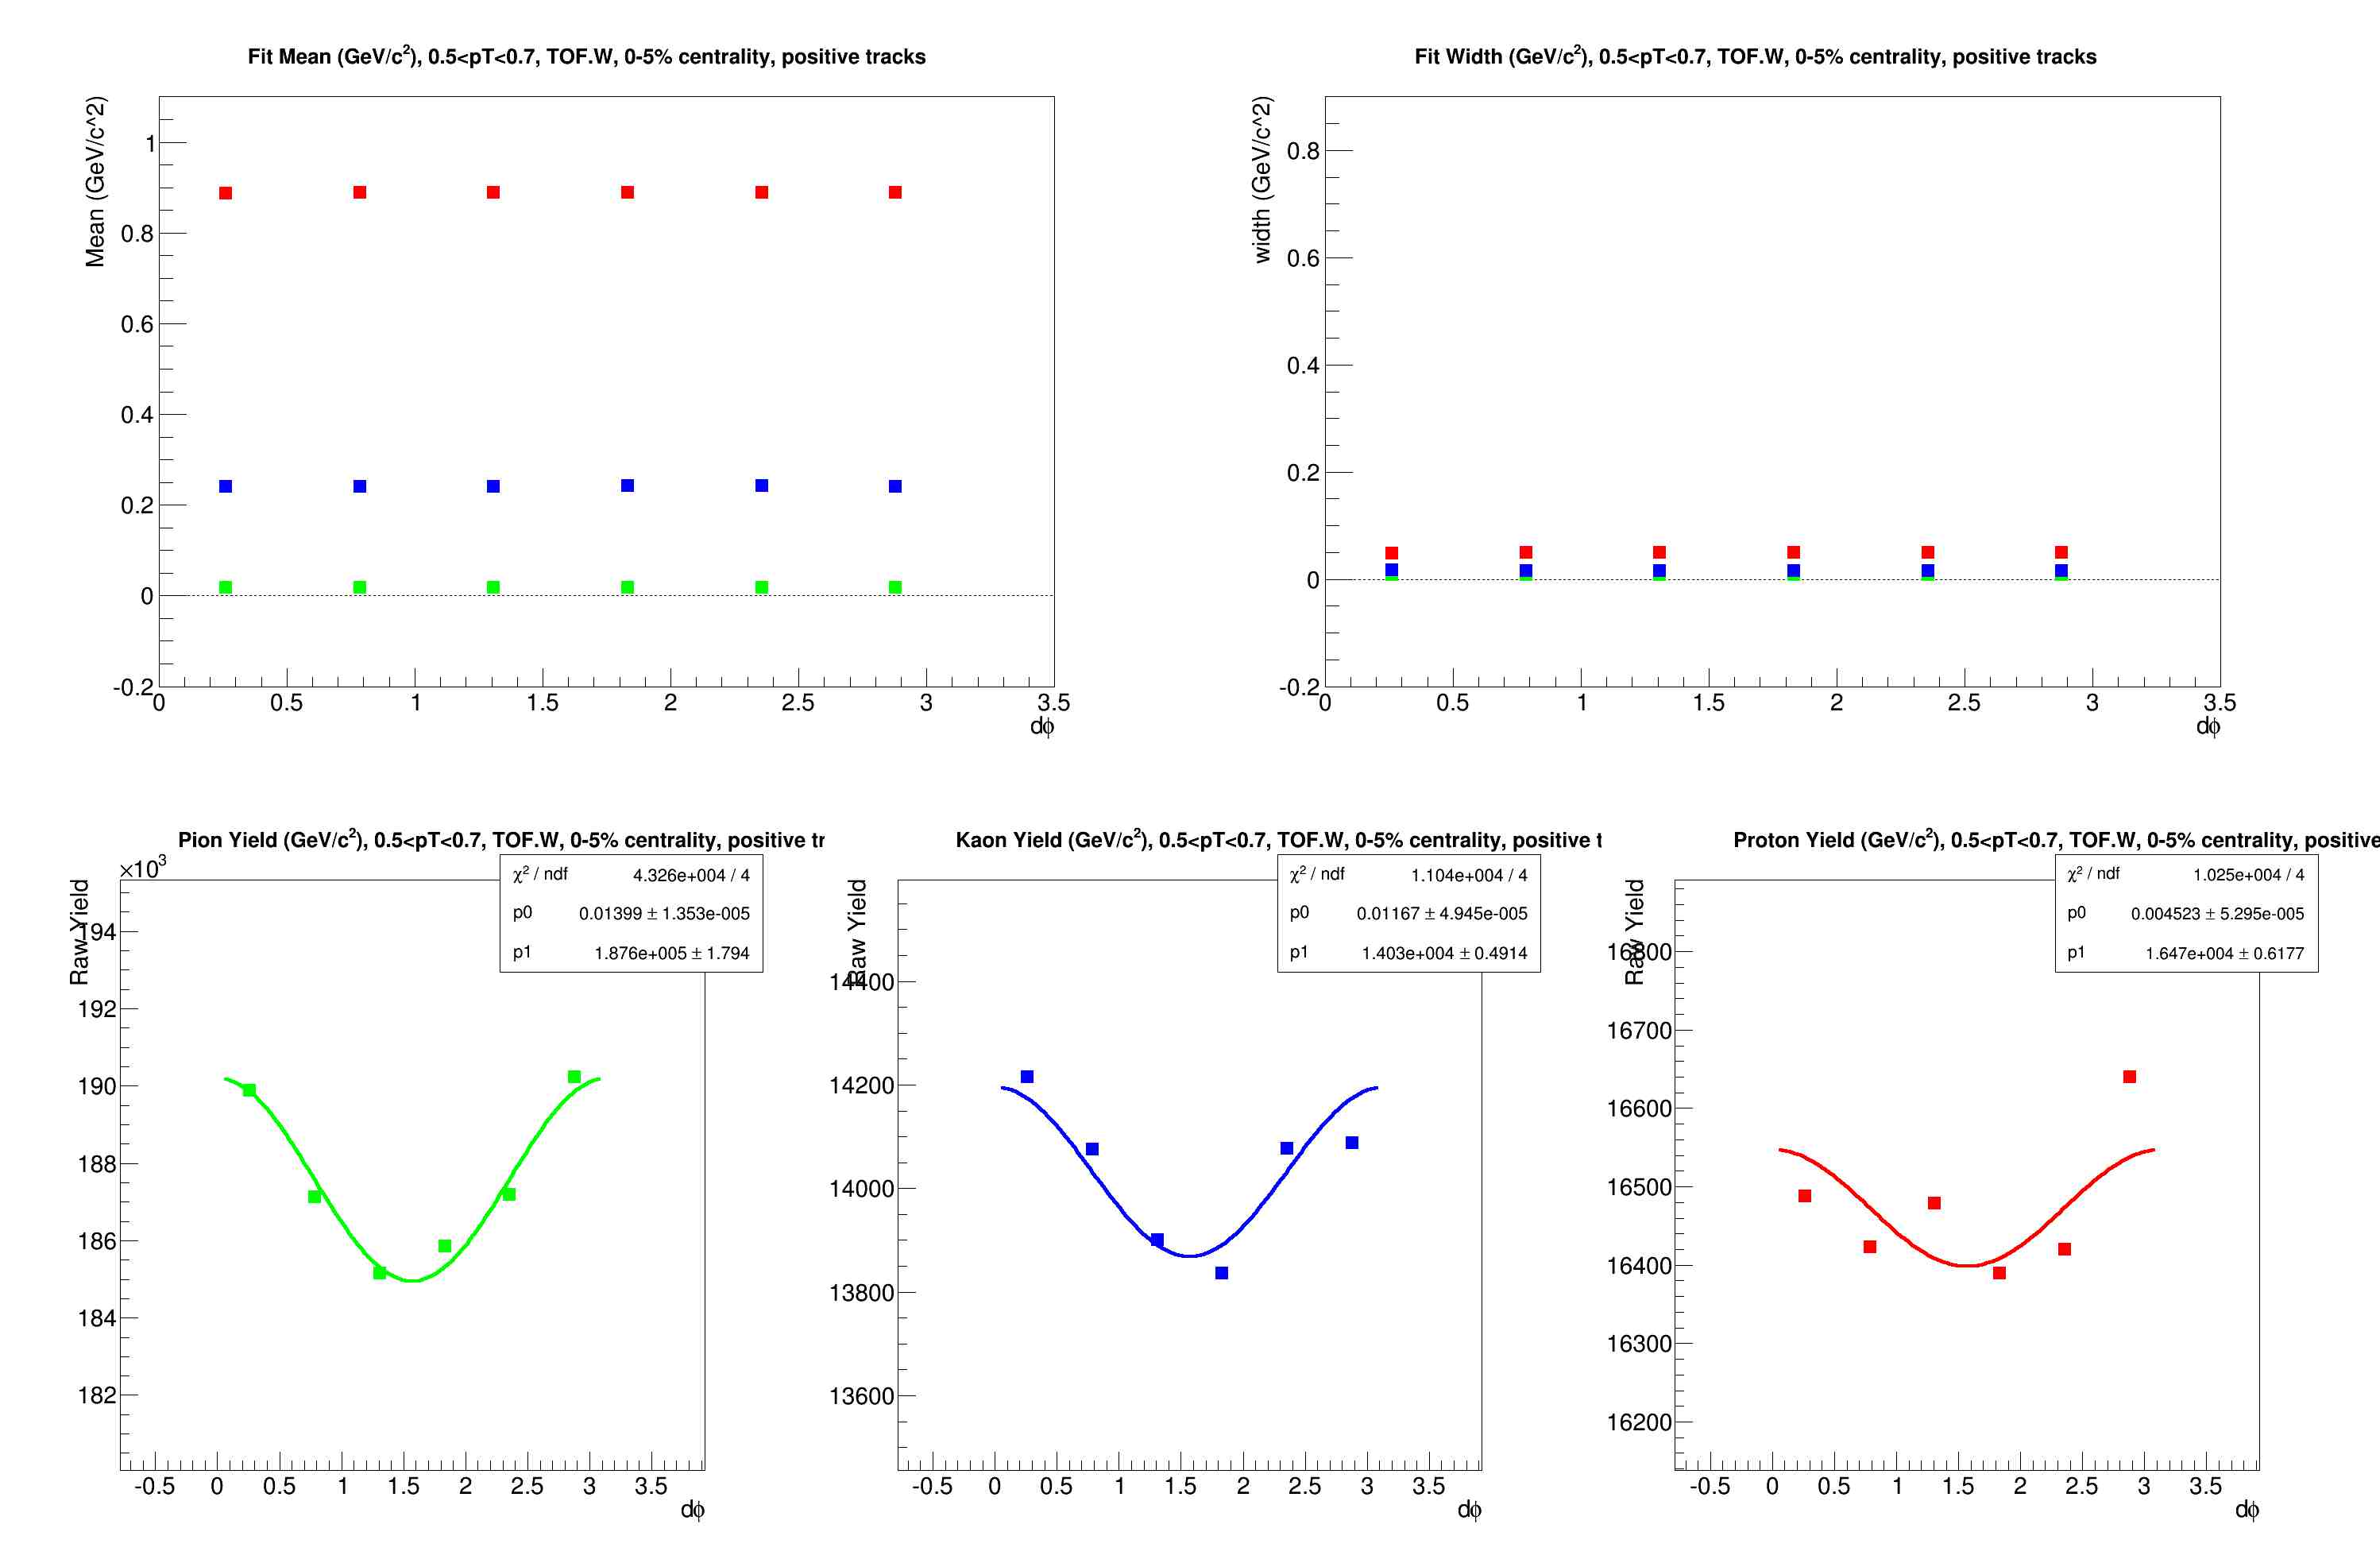
\includegraphics[width=1\textwidth]{lowptfits/fitParams_tof1_cent0_ch1_pT-5-7.jpg}
    \end{subfigure}
    \rule{35em}{0.5pt}
  \caption[PID fits and Yield vs $d\phi$ for $p_T$=0.5-0.7 GeV/c, TOF.W, positive particles ]{$m^2$ Gaussian fits for PID and resulting Yield vs $d\phi$ for $p_T$=0.5-0.7 GeV/c, TOF.W, positive particles}
  \label{fig:fits5-7pos}
\end{figure}

\begin{figure}[H]
  \centering
    \begin{subfigure}[p]{1\textwidth}
    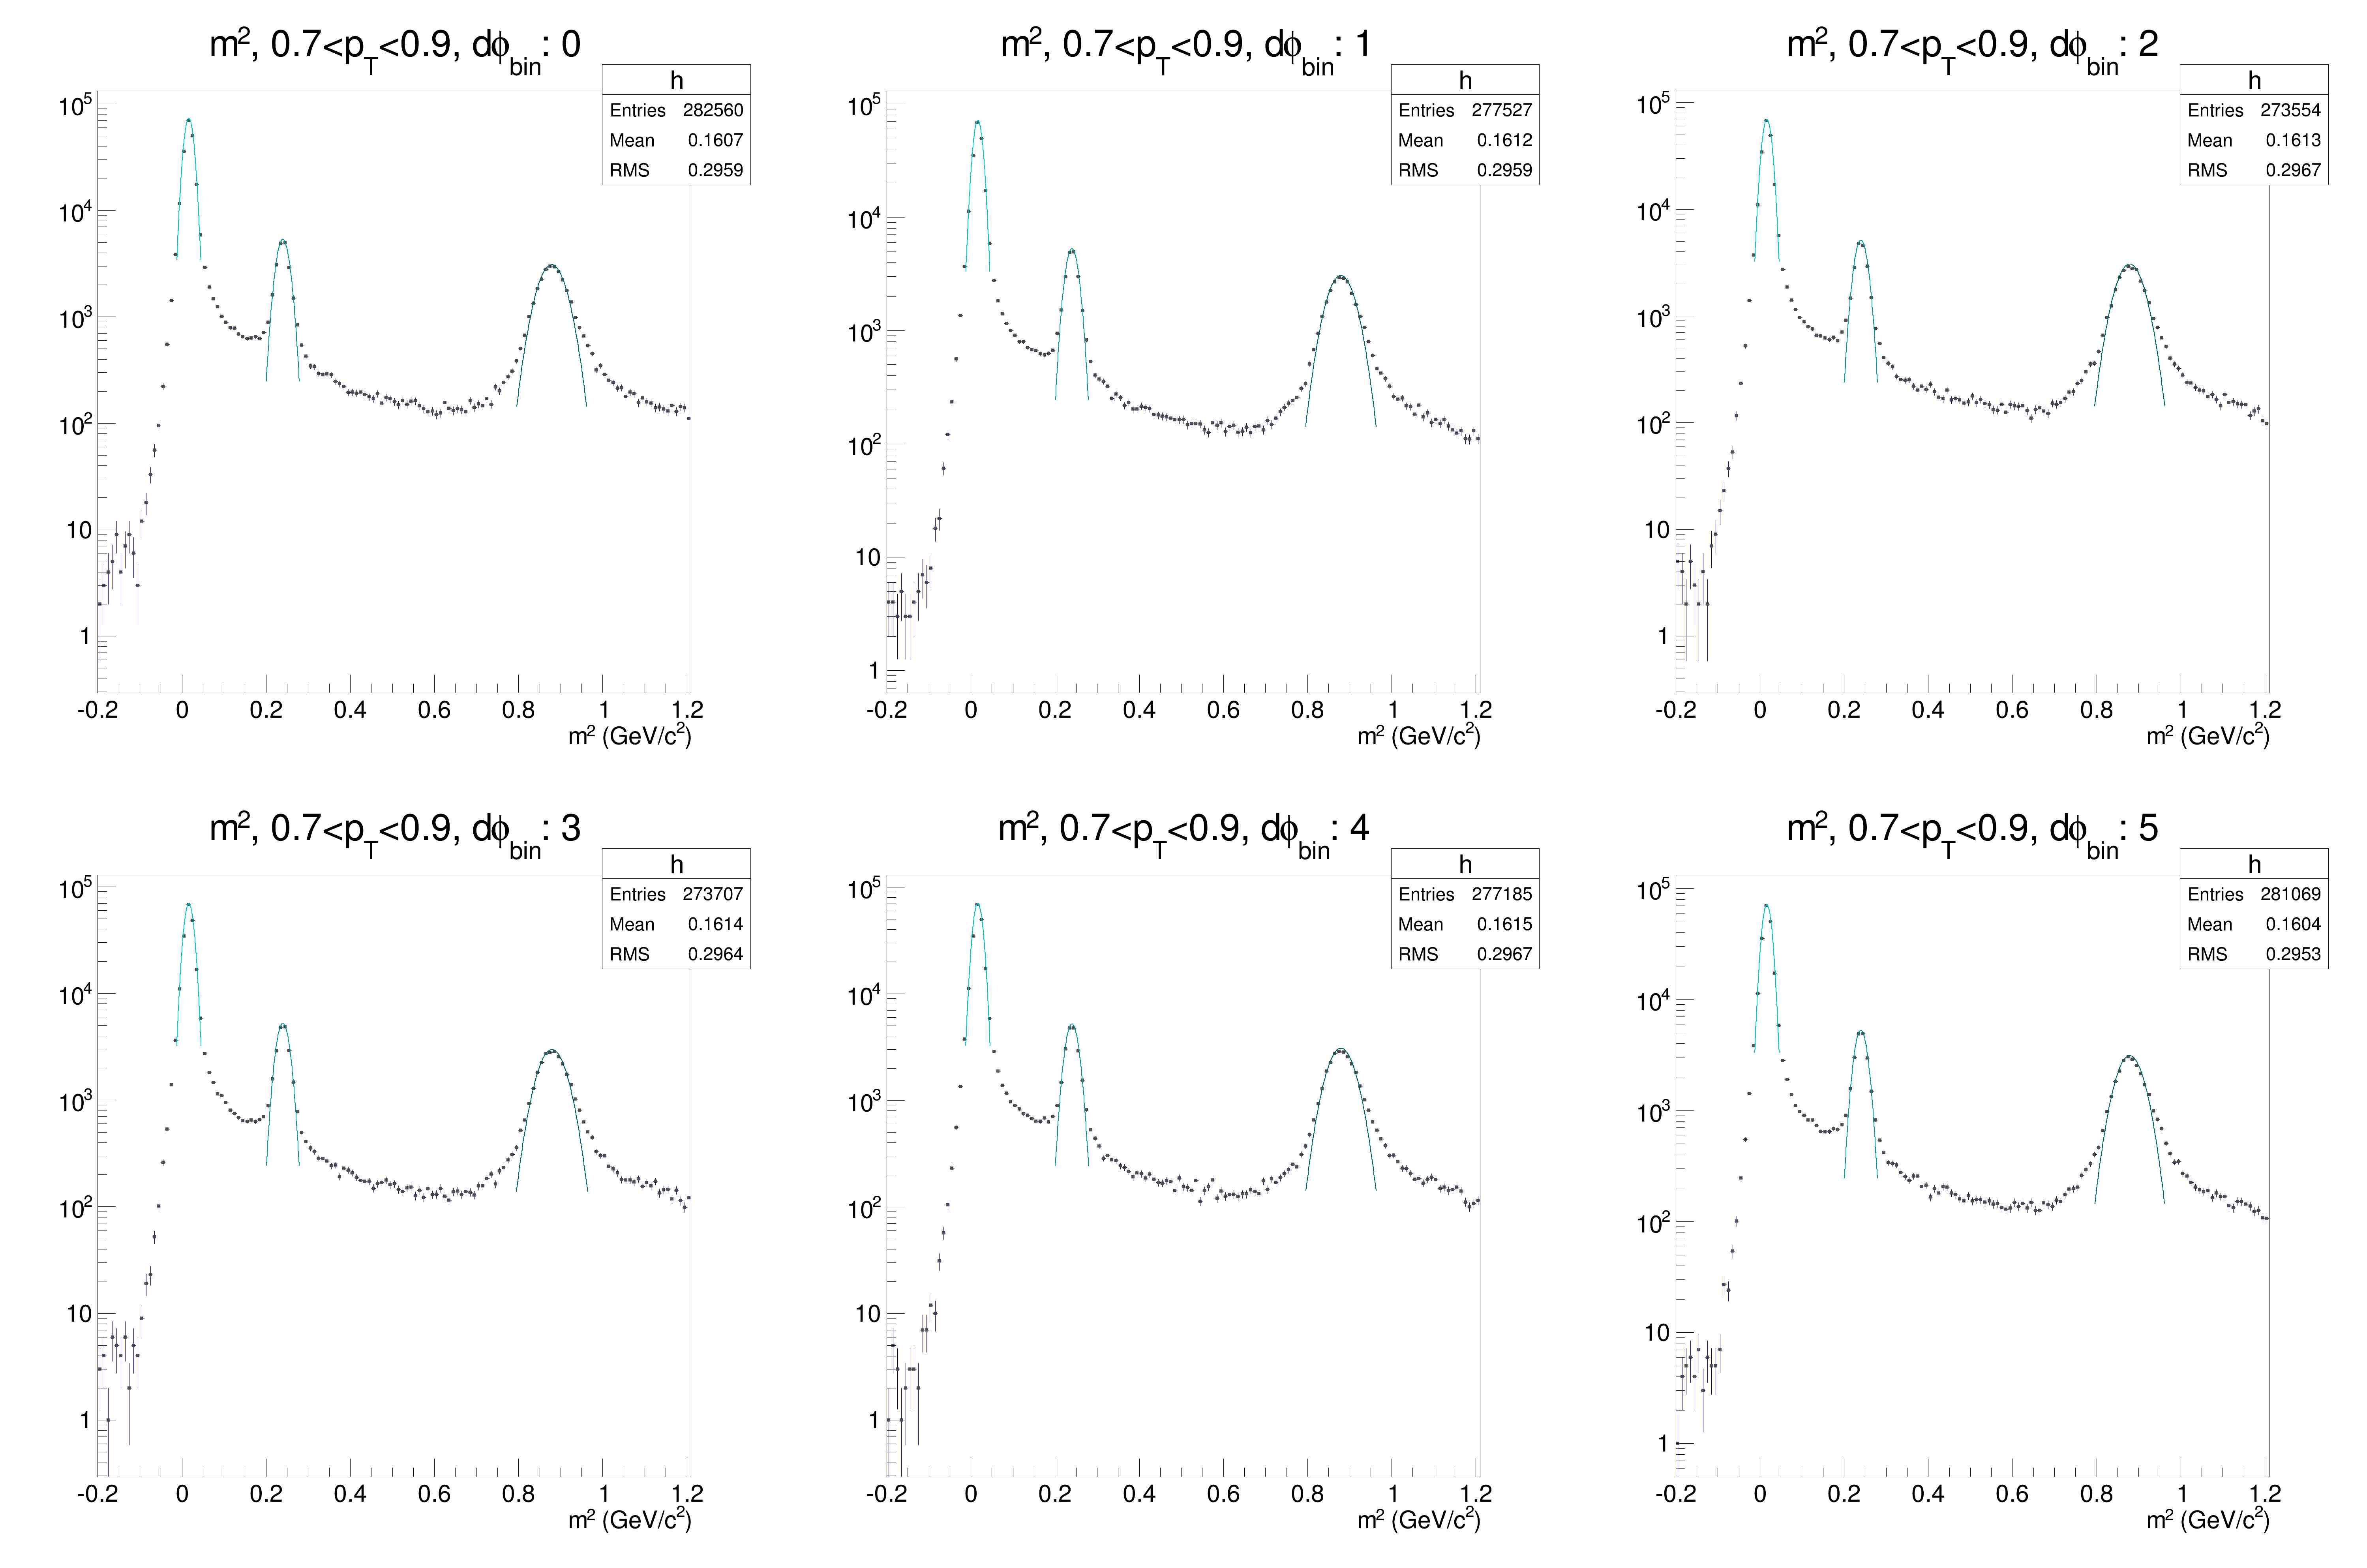
\includegraphics[width=1\textwidth]{lowptfits/yieldvsdphi_tof1_cent0_ch1_pT-7-9.jpg}
    \end{subfigure}
    \begin{subfigure}[p]{1\textwidth}
    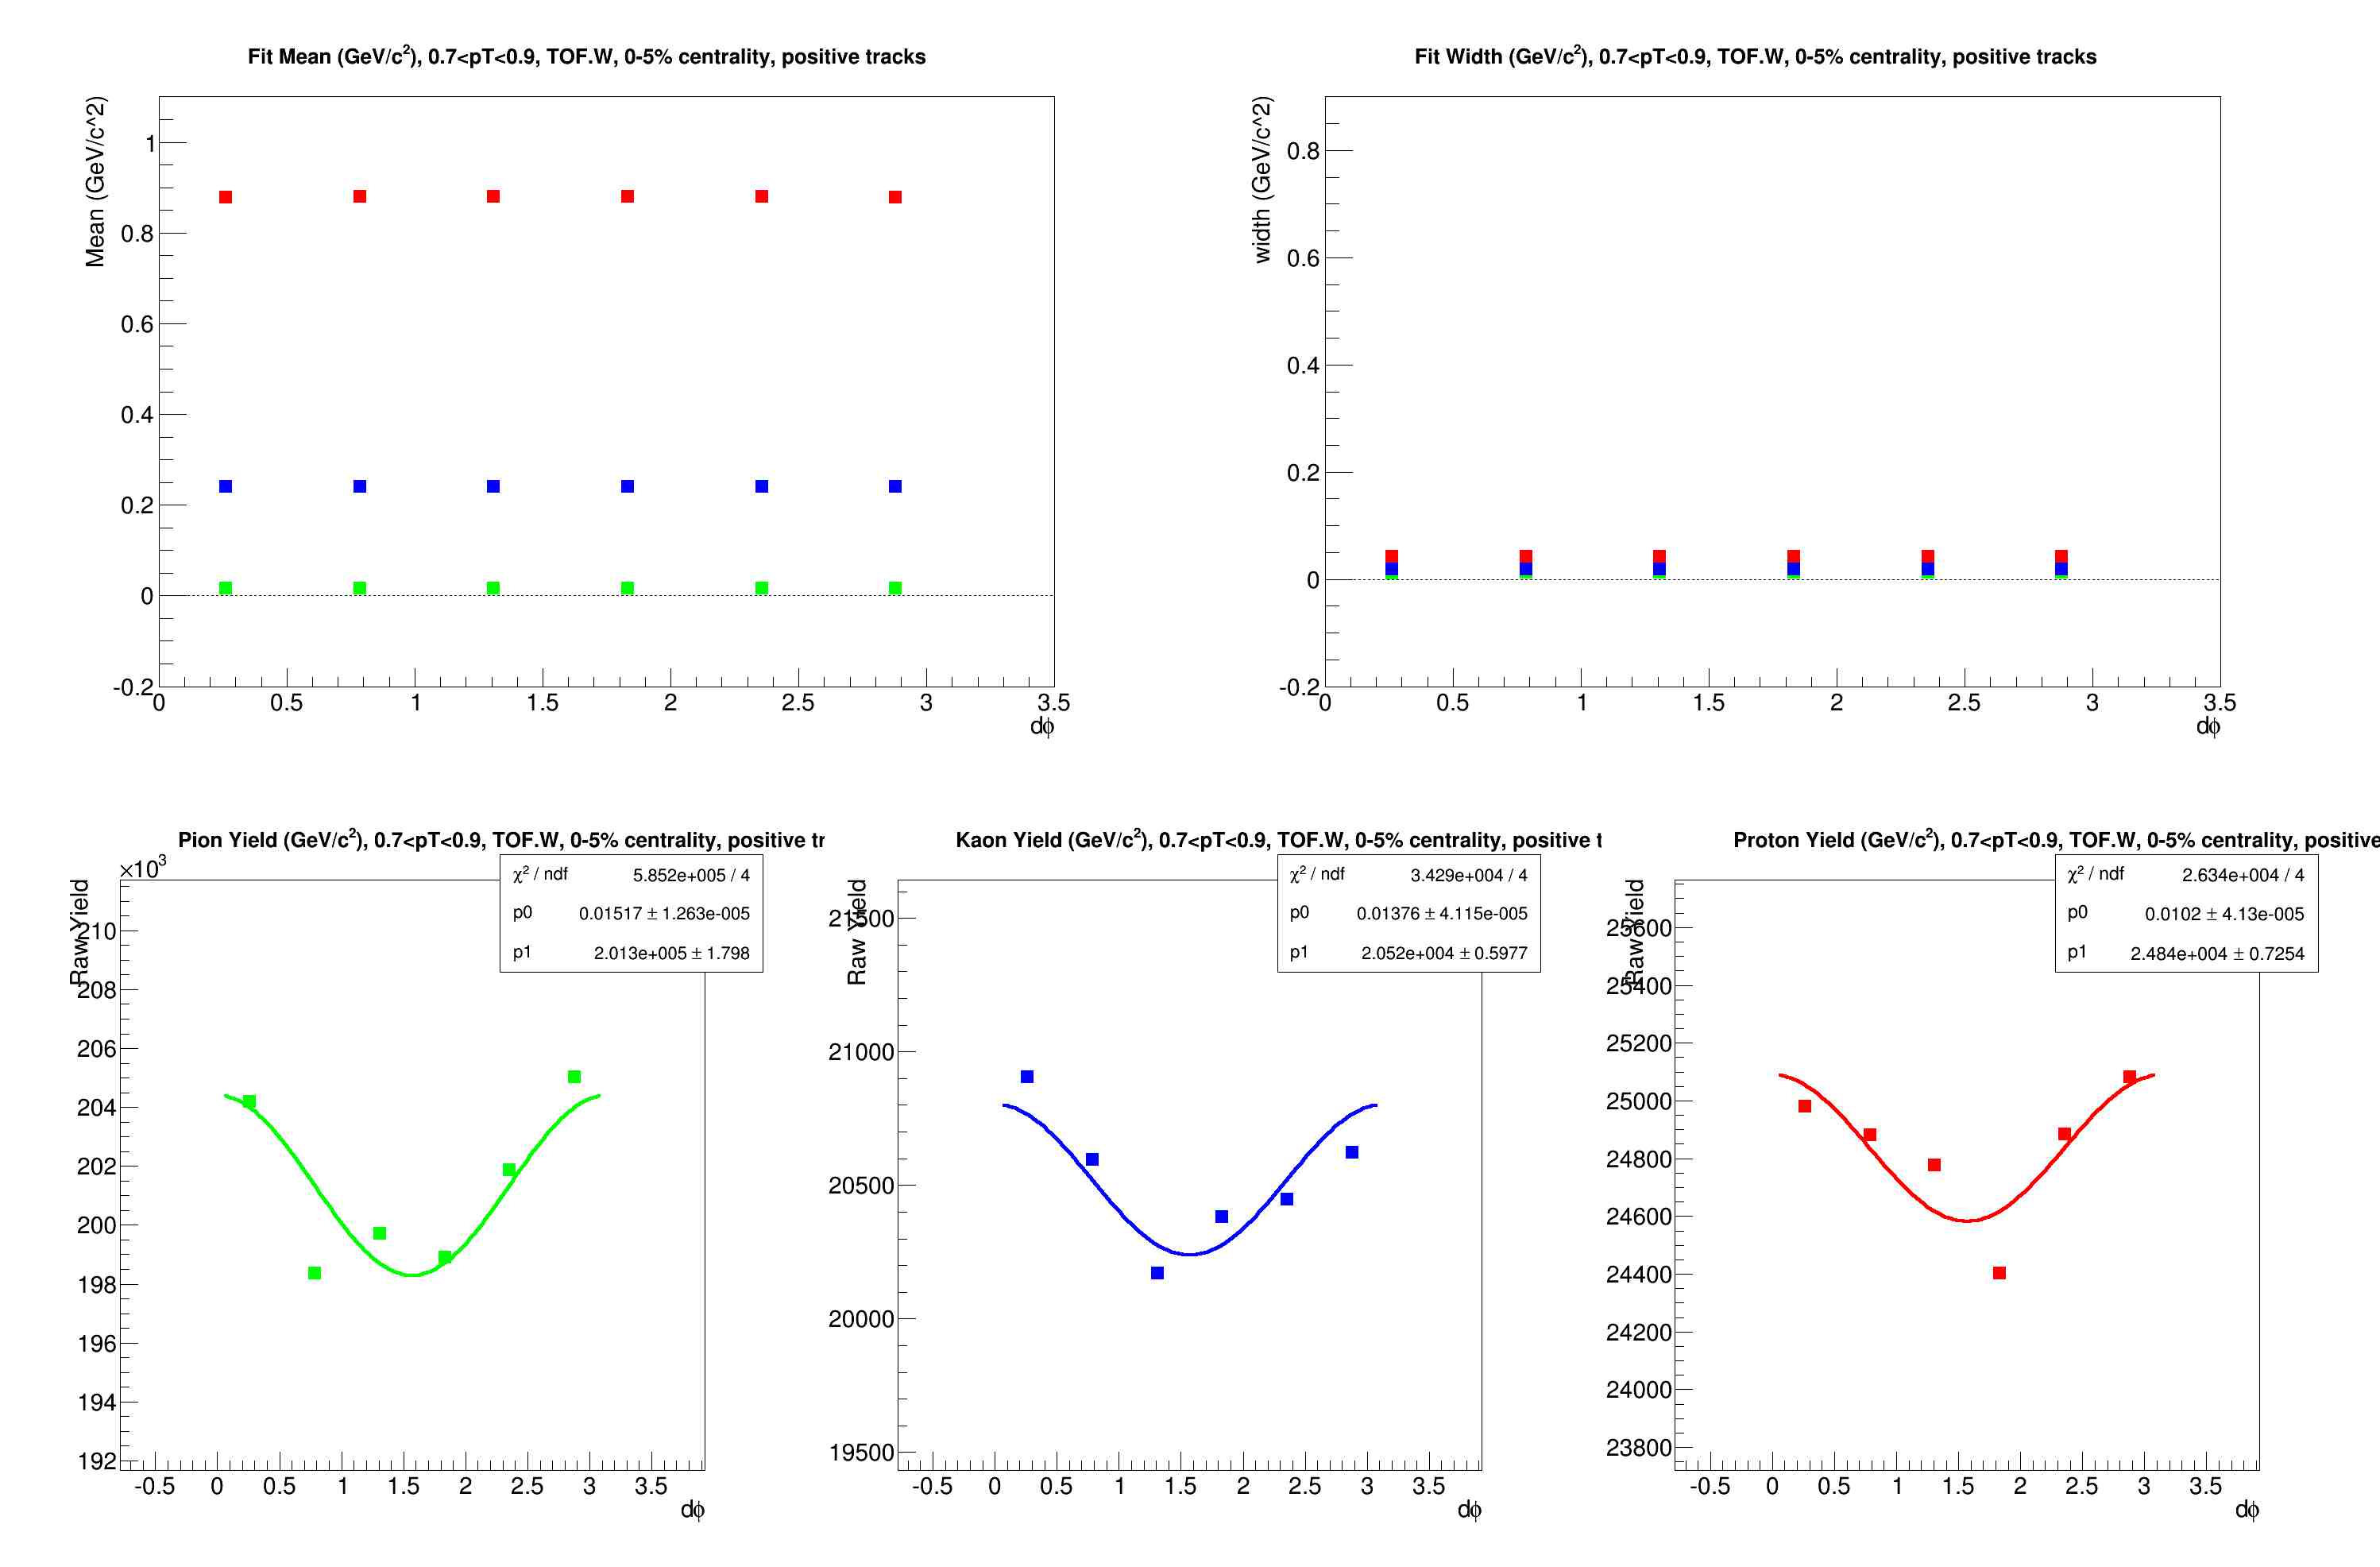
\includegraphics[width=1\textwidth]{lowptfits/fitParams_tof1_cent0_ch1_pT-7-9.jpg}
    \end{subfigure}
    \rule{35em}{0.5pt}
  \caption[PID fits and Yield vs $d\phi$ for $p_T$=0.7-0.9 GeV/c, TOF.W, positive particles ]{$m^2$ Gaussian fits for PID and resulting Yield vs $d\phi$ for $p_T$=0.7-0.9 GeV/c, TOF.W, positive particles}
  \label{fig:fits7-9pos}
\end{figure}

\begin{figure}[H]
  \centering
    \begin{subfigure}[p]{1\textwidth}
    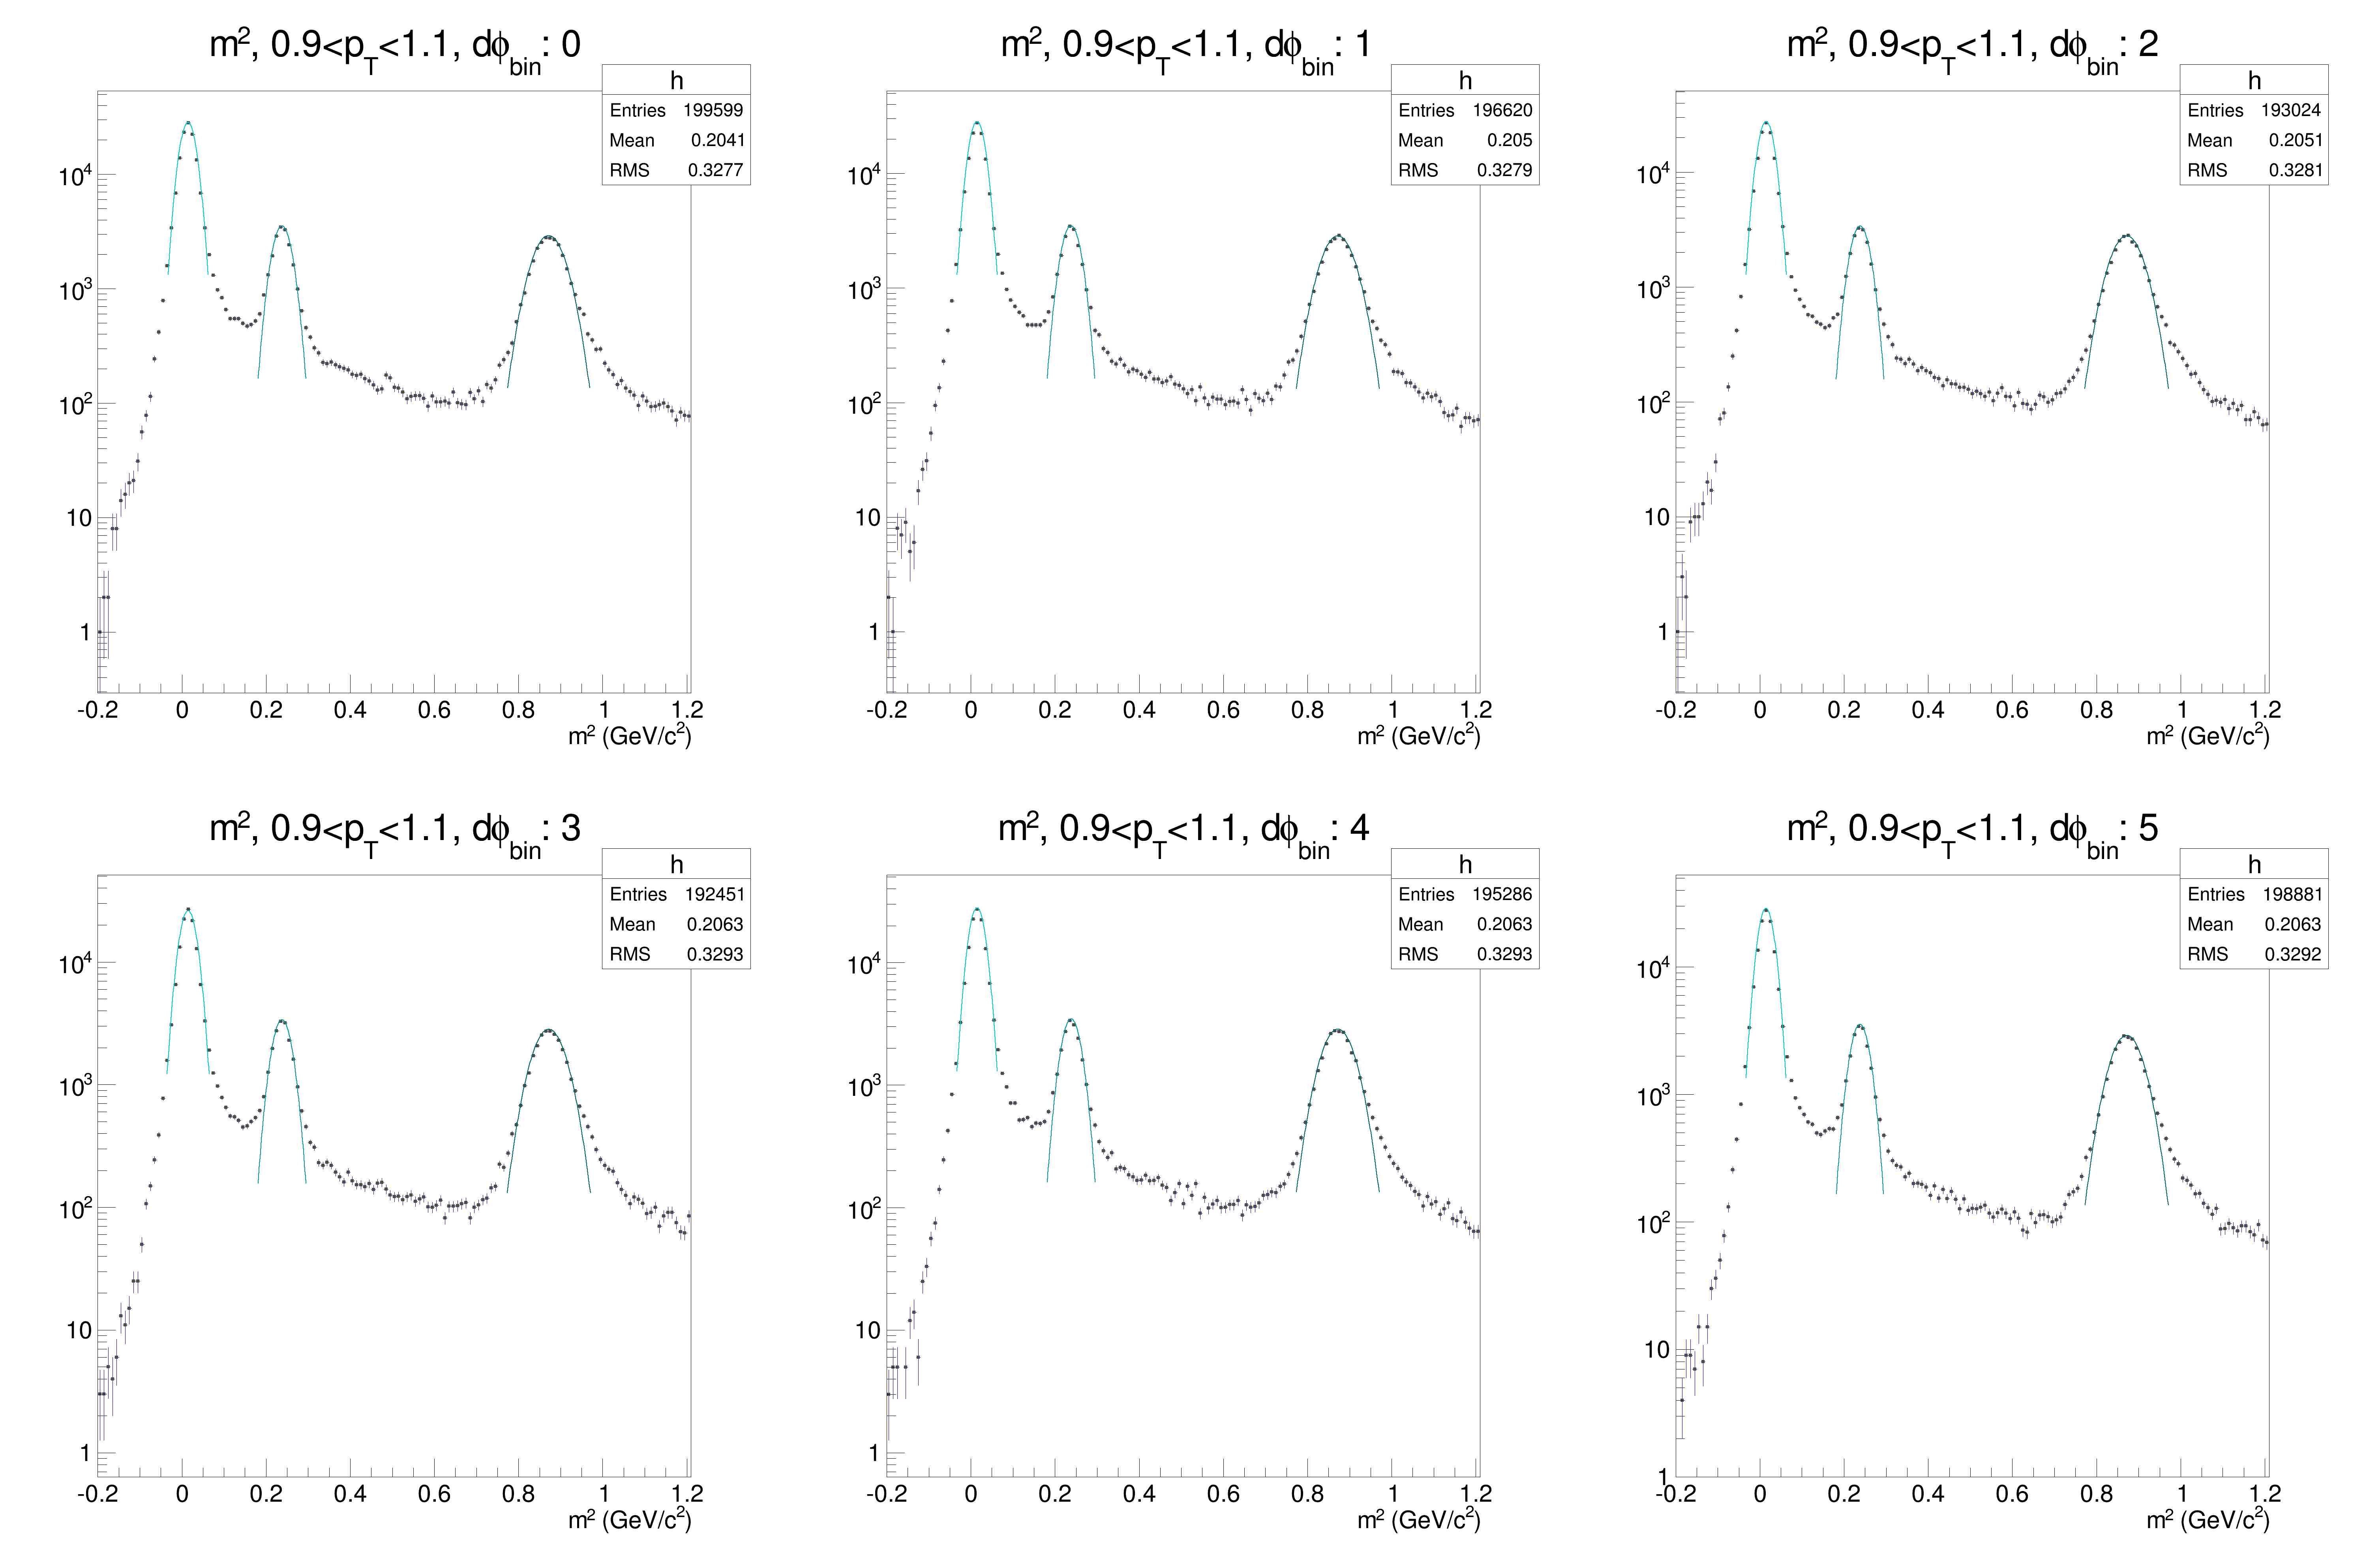
\includegraphics[width=1\textwidth]{lowptfits/yieldvsdphi_tof1_cent0_ch1_pT-9-11.jpg}
    \end{subfigure}
    \begin{subfigure}[p]{1\textwidth}
    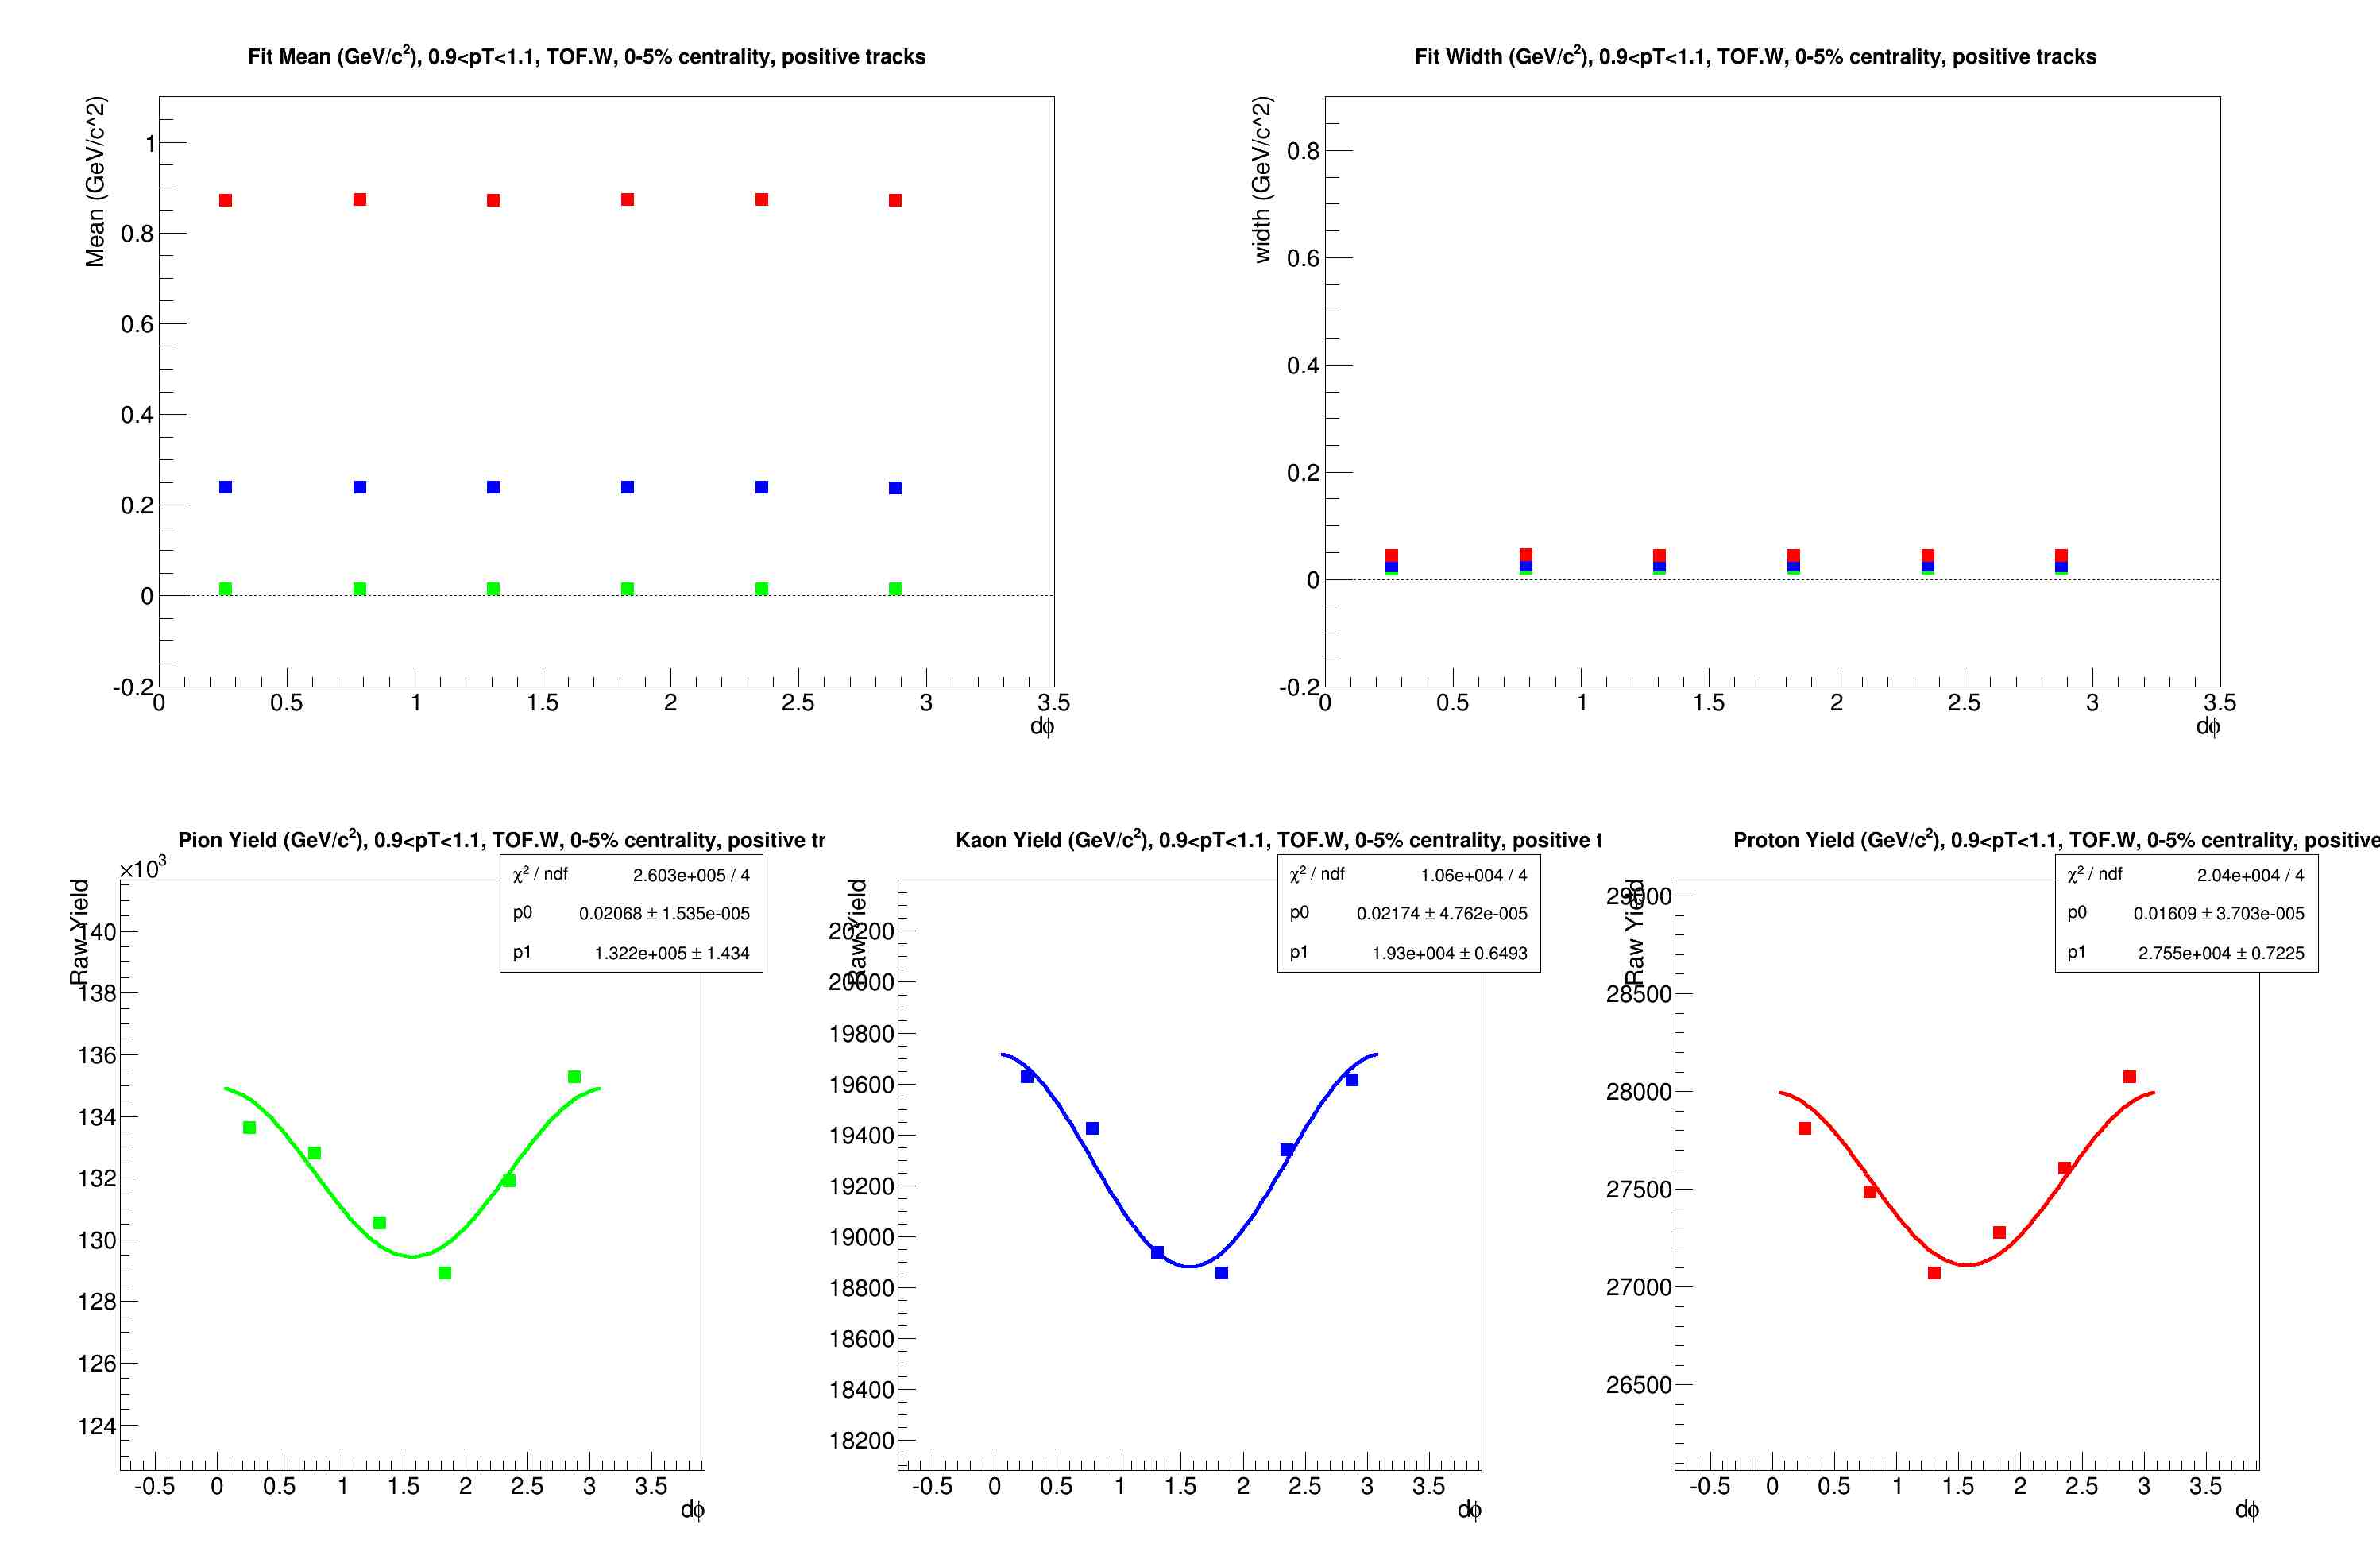
\includegraphics[width=1\textwidth]{lowptfits/fitParams_tof1_cent0_ch1_pT-9-11.jpg}
    \end{subfigure}
    \rule{35em}{0.5pt}
  \caption[PID fits and Yield vs $d\phi$ for $p_T$=0.9-1.1 GeV/c, TOF.W, positive particles ]{$m^2$ Gaussian fits for PID and resulting Yield vs $d\phi$ for $p_T$=0.9-1.1 GeV/c, TOF.W, positive particles}
  \label{fig:fits9-11pos}
\end{figure}

\begin{figure}[H]
  \centering
    \begin{subfigure}[p]{1\textwidth}
    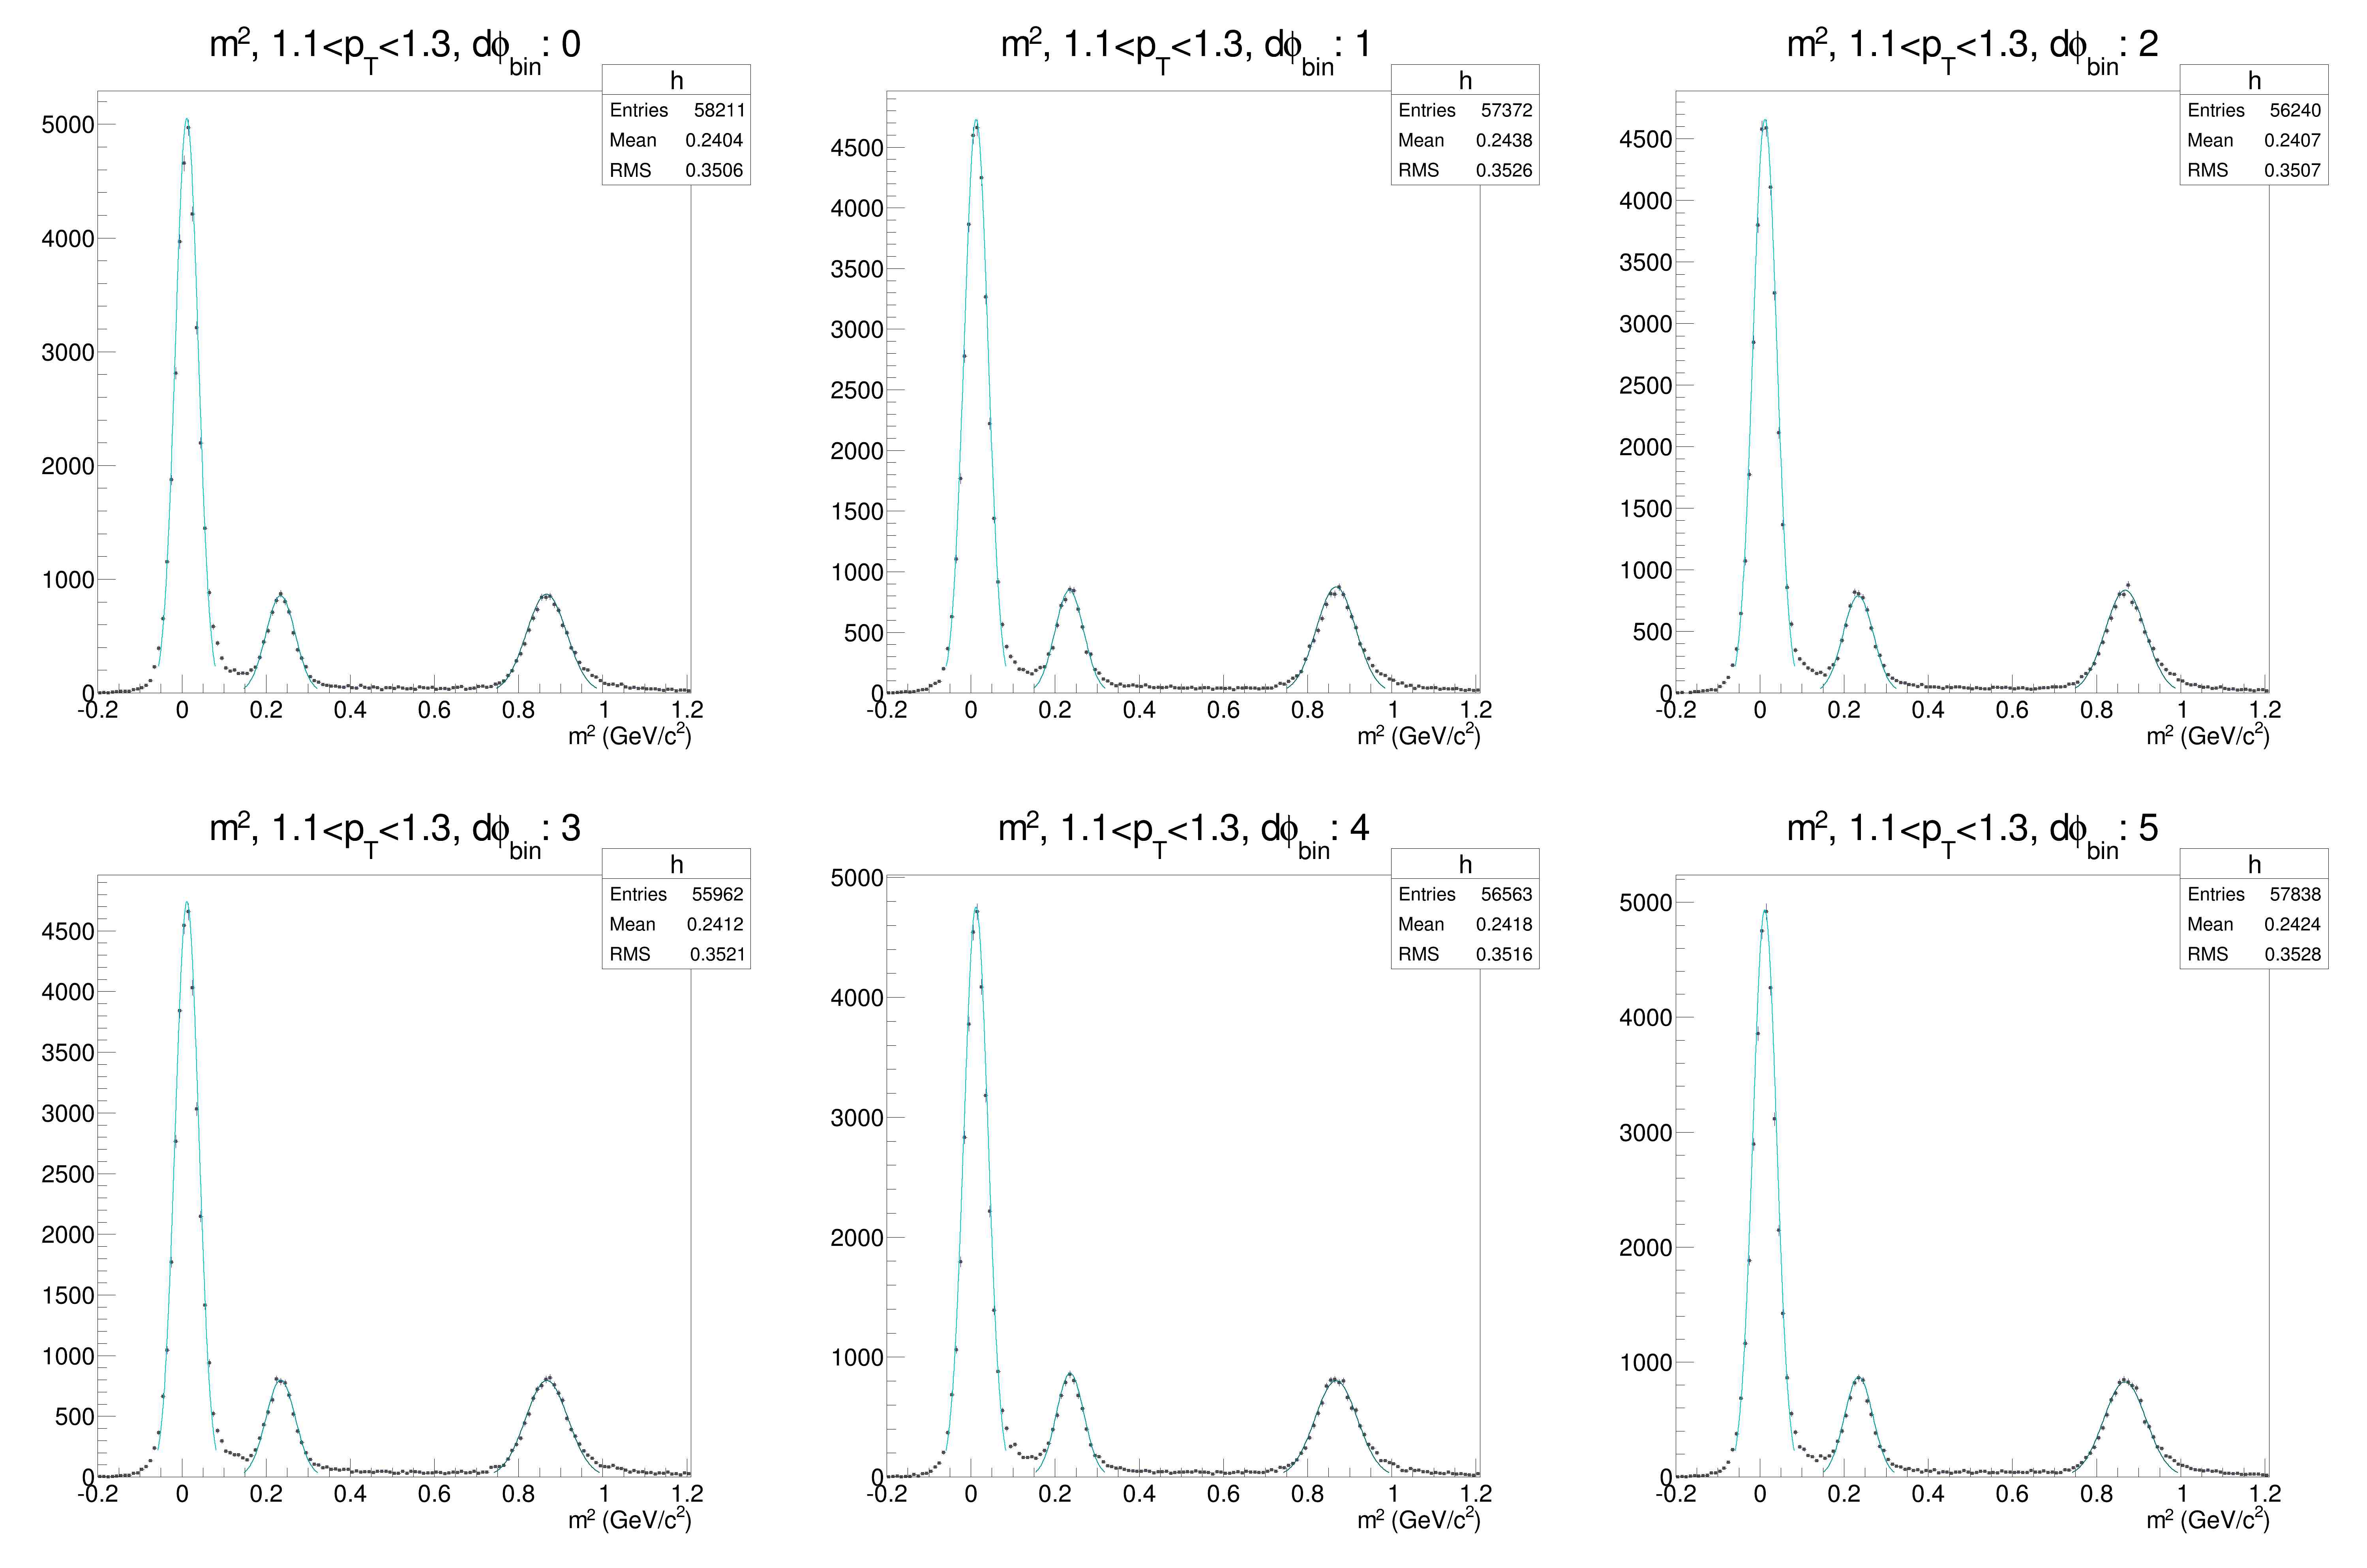
\includegraphics[width=1\textwidth]{lowptfits/yieldvsdphi_tof1_cent0_ch1_pT-11-13.jpg}
    \end{subfigure}
    \begin{subfigure}[p]{1\textwidth}
    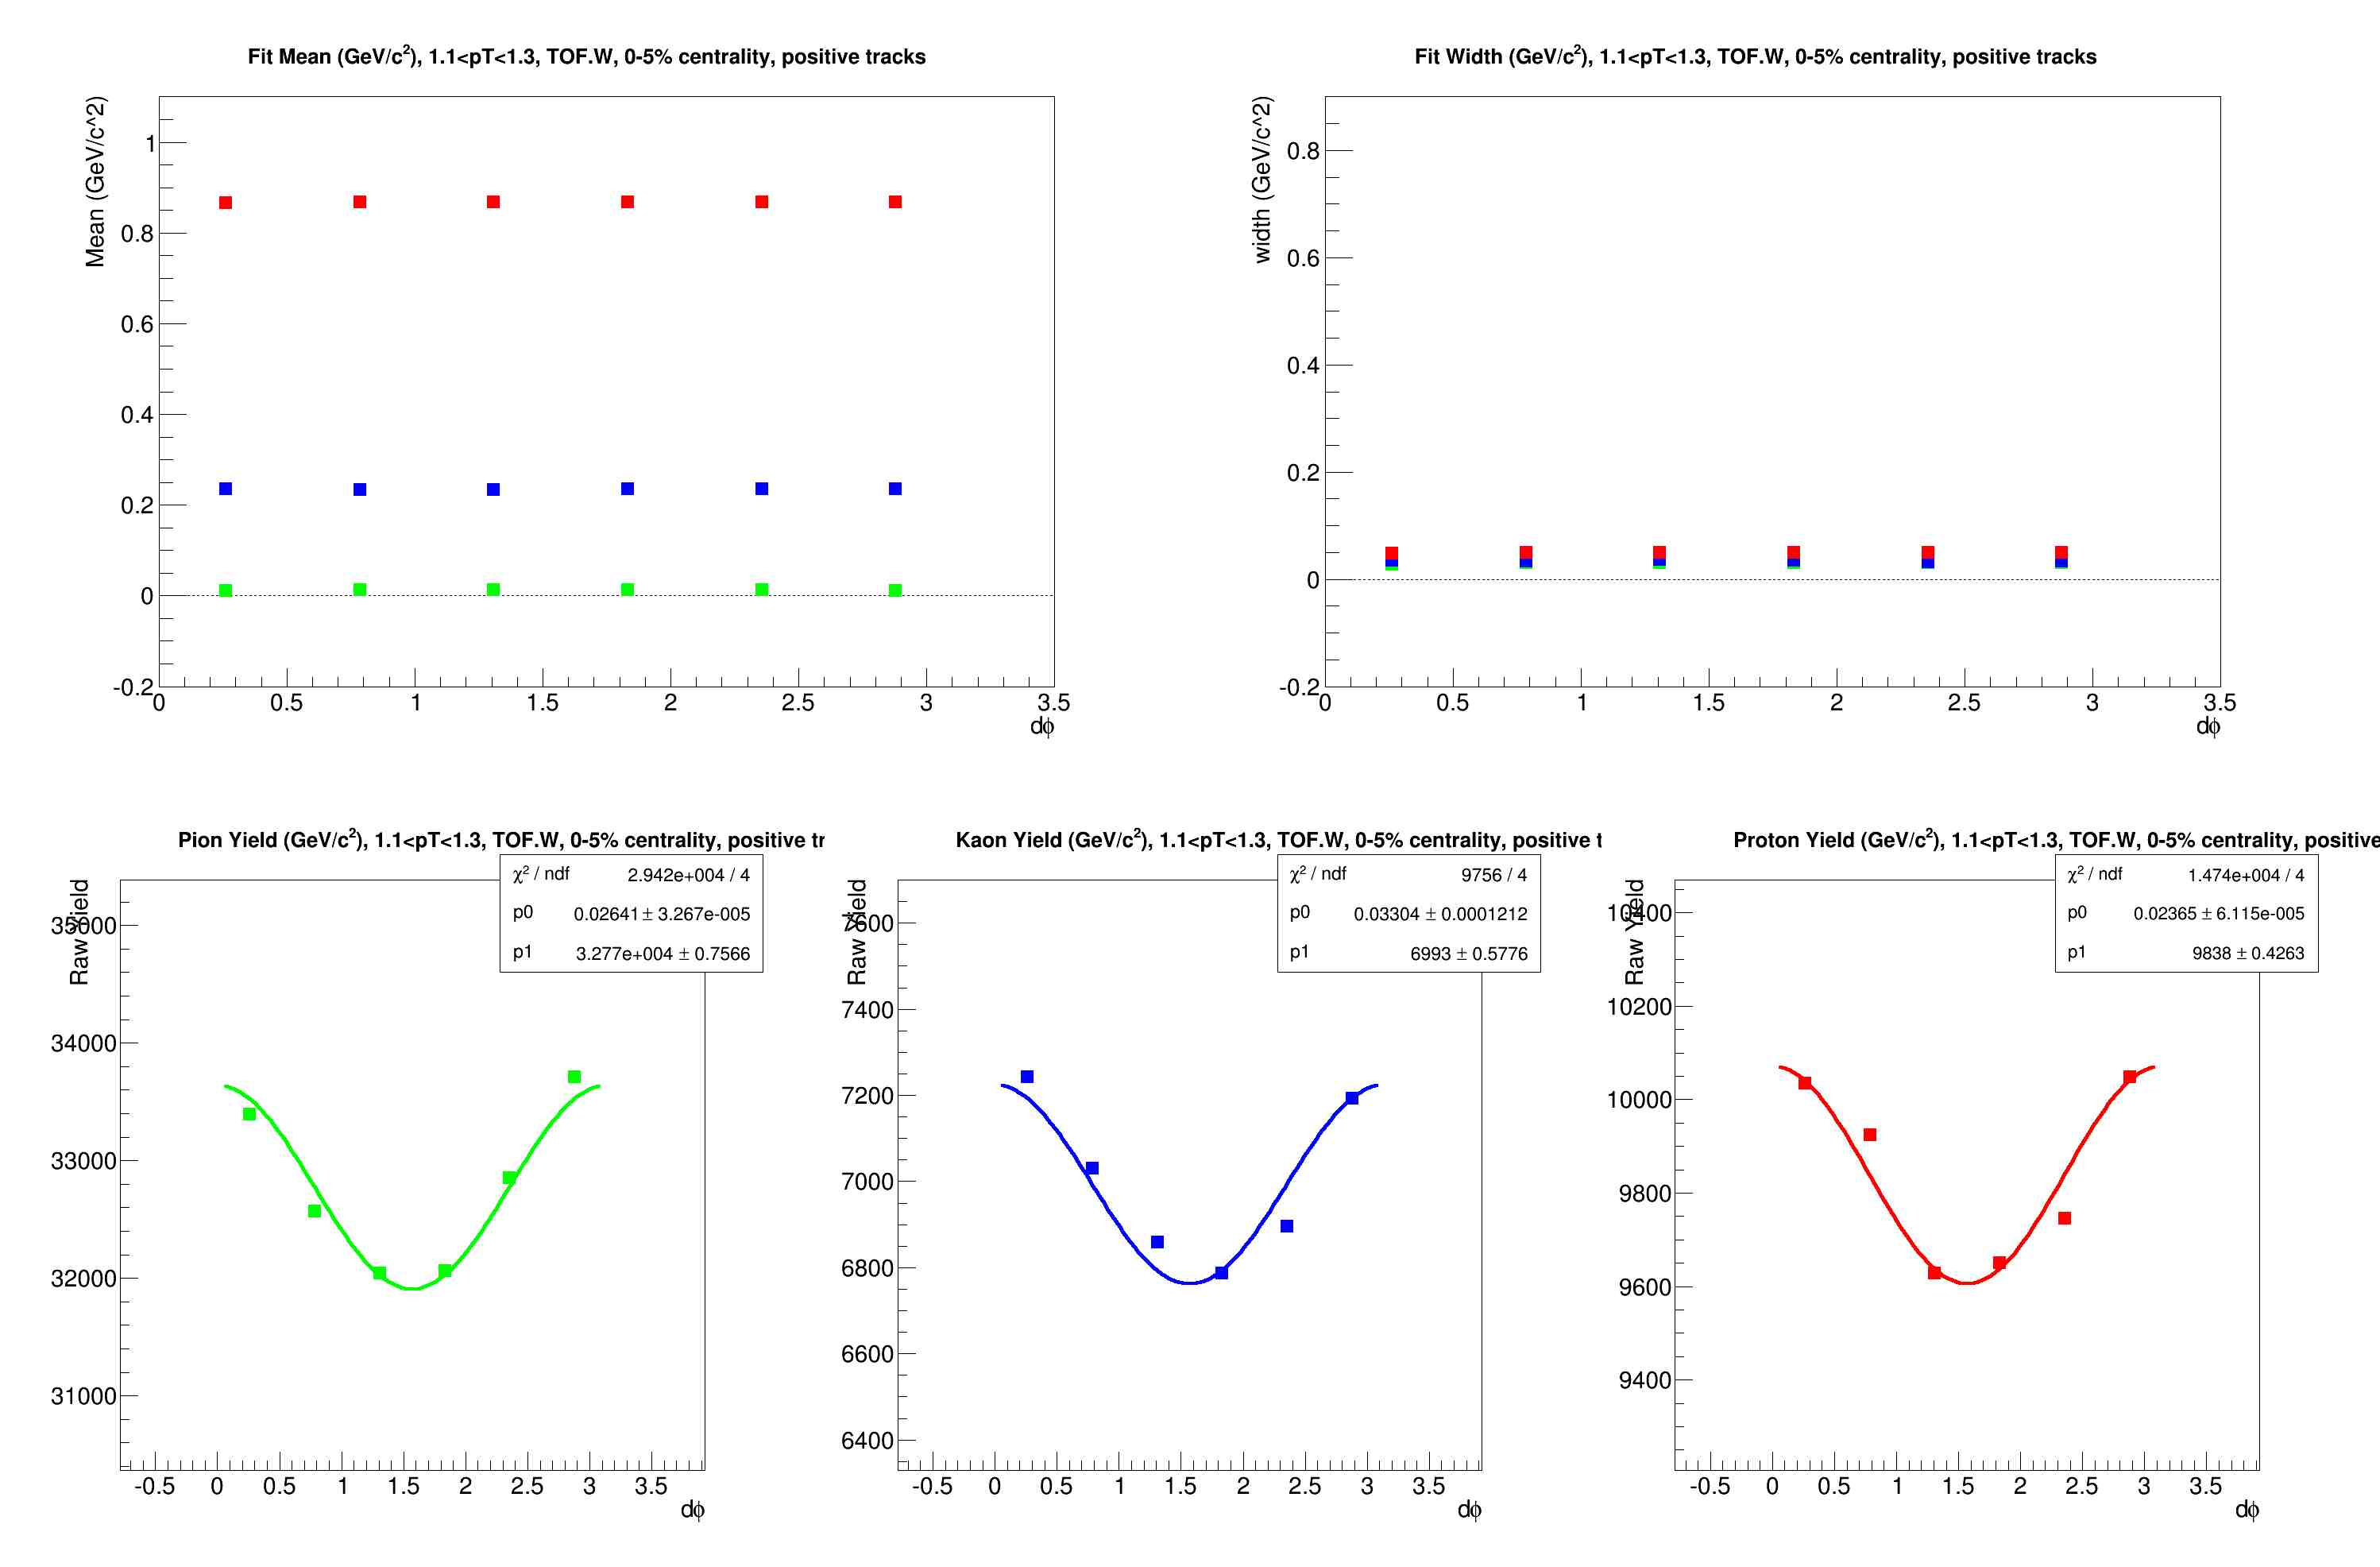
\includegraphics[width=1\textwidth]{lowptfits/fitParams_tof1_cent0_ch1_pT-11-13.jpg}
    \end{subfigure}
    \rule{35em}{0.5pt}
  \caption[PID fits and Yield vs $d\phi$ for $p_T$=1.1-1.3 GeV/c, TOF.W, positive particles ]{$m^2$ Gaussian fits for PID and resulting Yield vs $d\phi$ for $p_T$=1.1-1.3 GeV/c, TOF.W, positive particles}
  \label{fig:fits11-13pos}
\end{figure}
\restoregeometry


\subsection{Gaussian Mixing}
For $1.3<p_T<2.1$, kaon and pion mass distributions become overlapped. To decouple the two I use a mixed Gaussian model in order to fit the tails of the distributions without over counting. This function takes the form:

\begin{equation}
f(x) = \frac{1}{\sqrt{2\pi}} \bigg( \frac{N_{\pi}}{\sigma_{\pi}} e^{-\frac{(x-\mu_{\pi})^2}{2\sigma_{\pi}^{2}}} + \frac{N_{k}}{\sigma_{\pi}-\sigma_{k}} e^{-\frac{(x-\mu_{k})^2}{2(\sigma_{\pi} - \sigma_{k})^{2}}} \bigg),
\end{equation}
where $N_{x}$, $\mu_x$, and $\sigma_x$ are the parameters that describe the shape of particle $x$'s ($\pi$/k) distribution. These parameters can then be used to reconstruct single Gaussian distributions which are then integrated out to $2\sigma$ as mentioned in the previous section.

\newgeometry{top=2cm} 
\subsubsection{Mixed Gaussian fits, $p_T$=1.3-2.1 GeV/c, TOF.W, negative charged tracks}

\begin{figure}[H]
  \centering
    \begin{subfigure}{1\textwidth}
    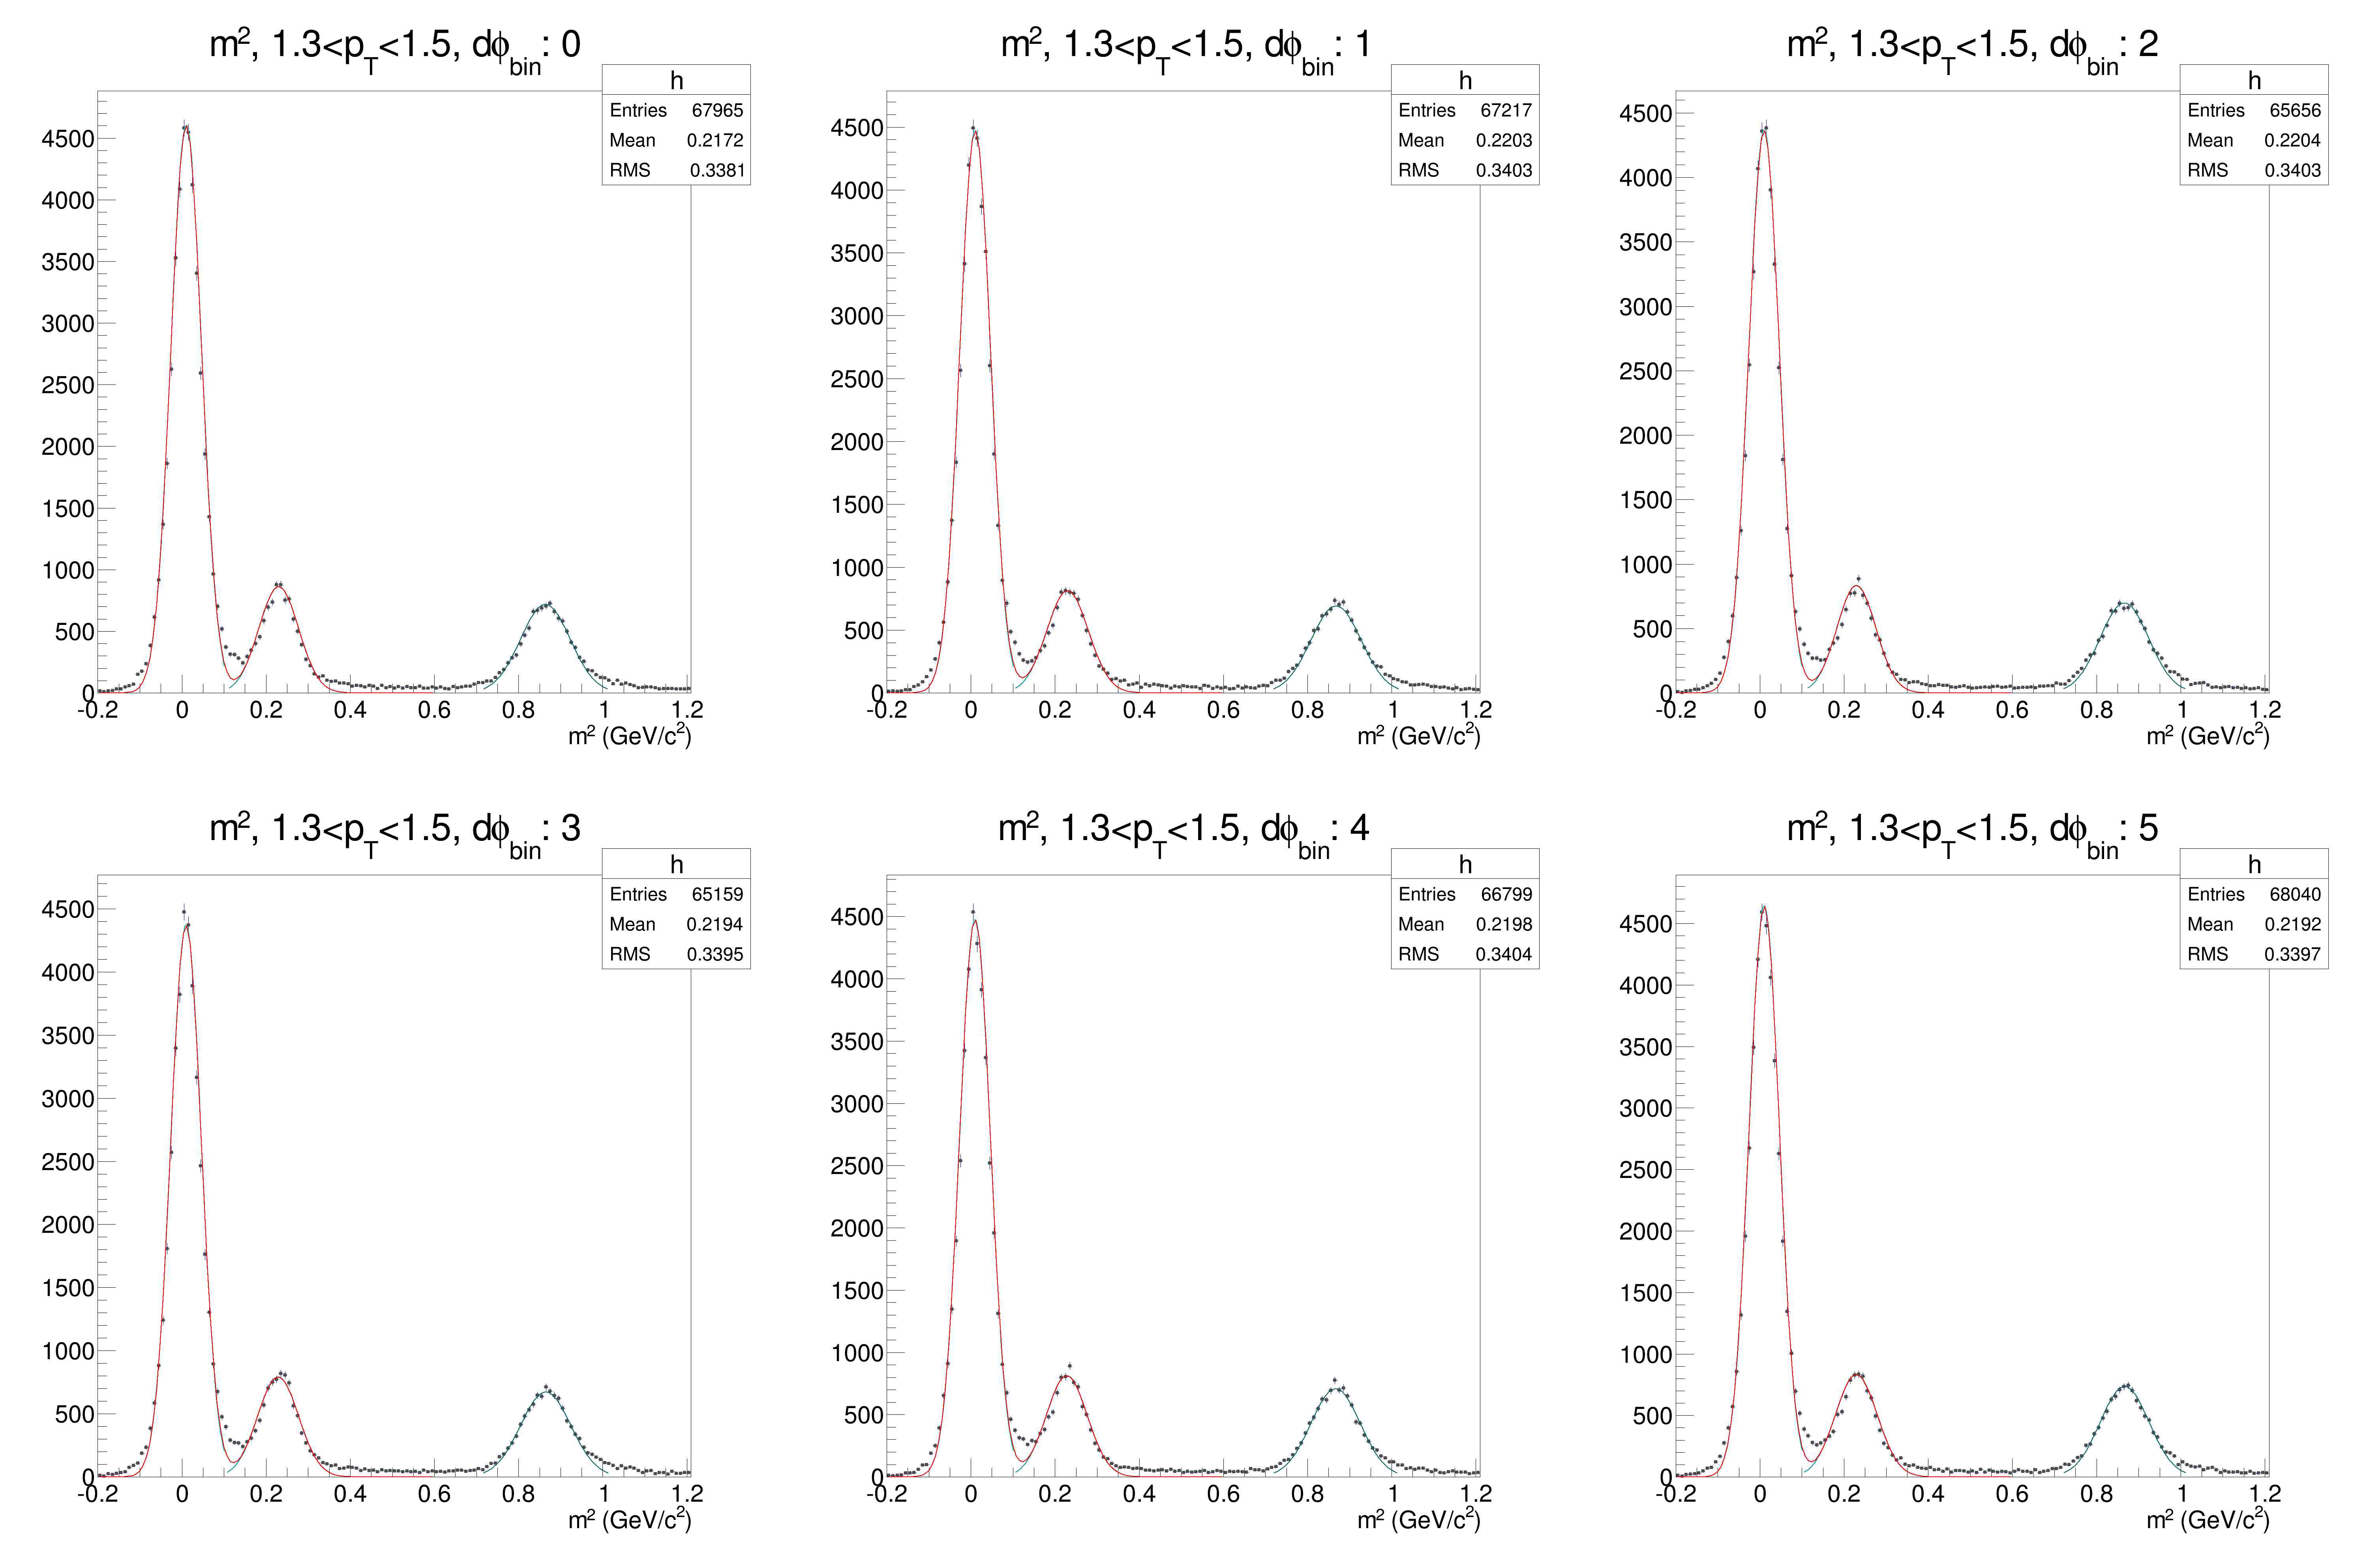
\includegraphics[width=1\textwidth]{lowptfits/yieldvsdphi_tof1_cent0_ch0_pT-13-15.jpg}
    \end{subfigure}
    \begin{subfigure}{1\textwidth}
    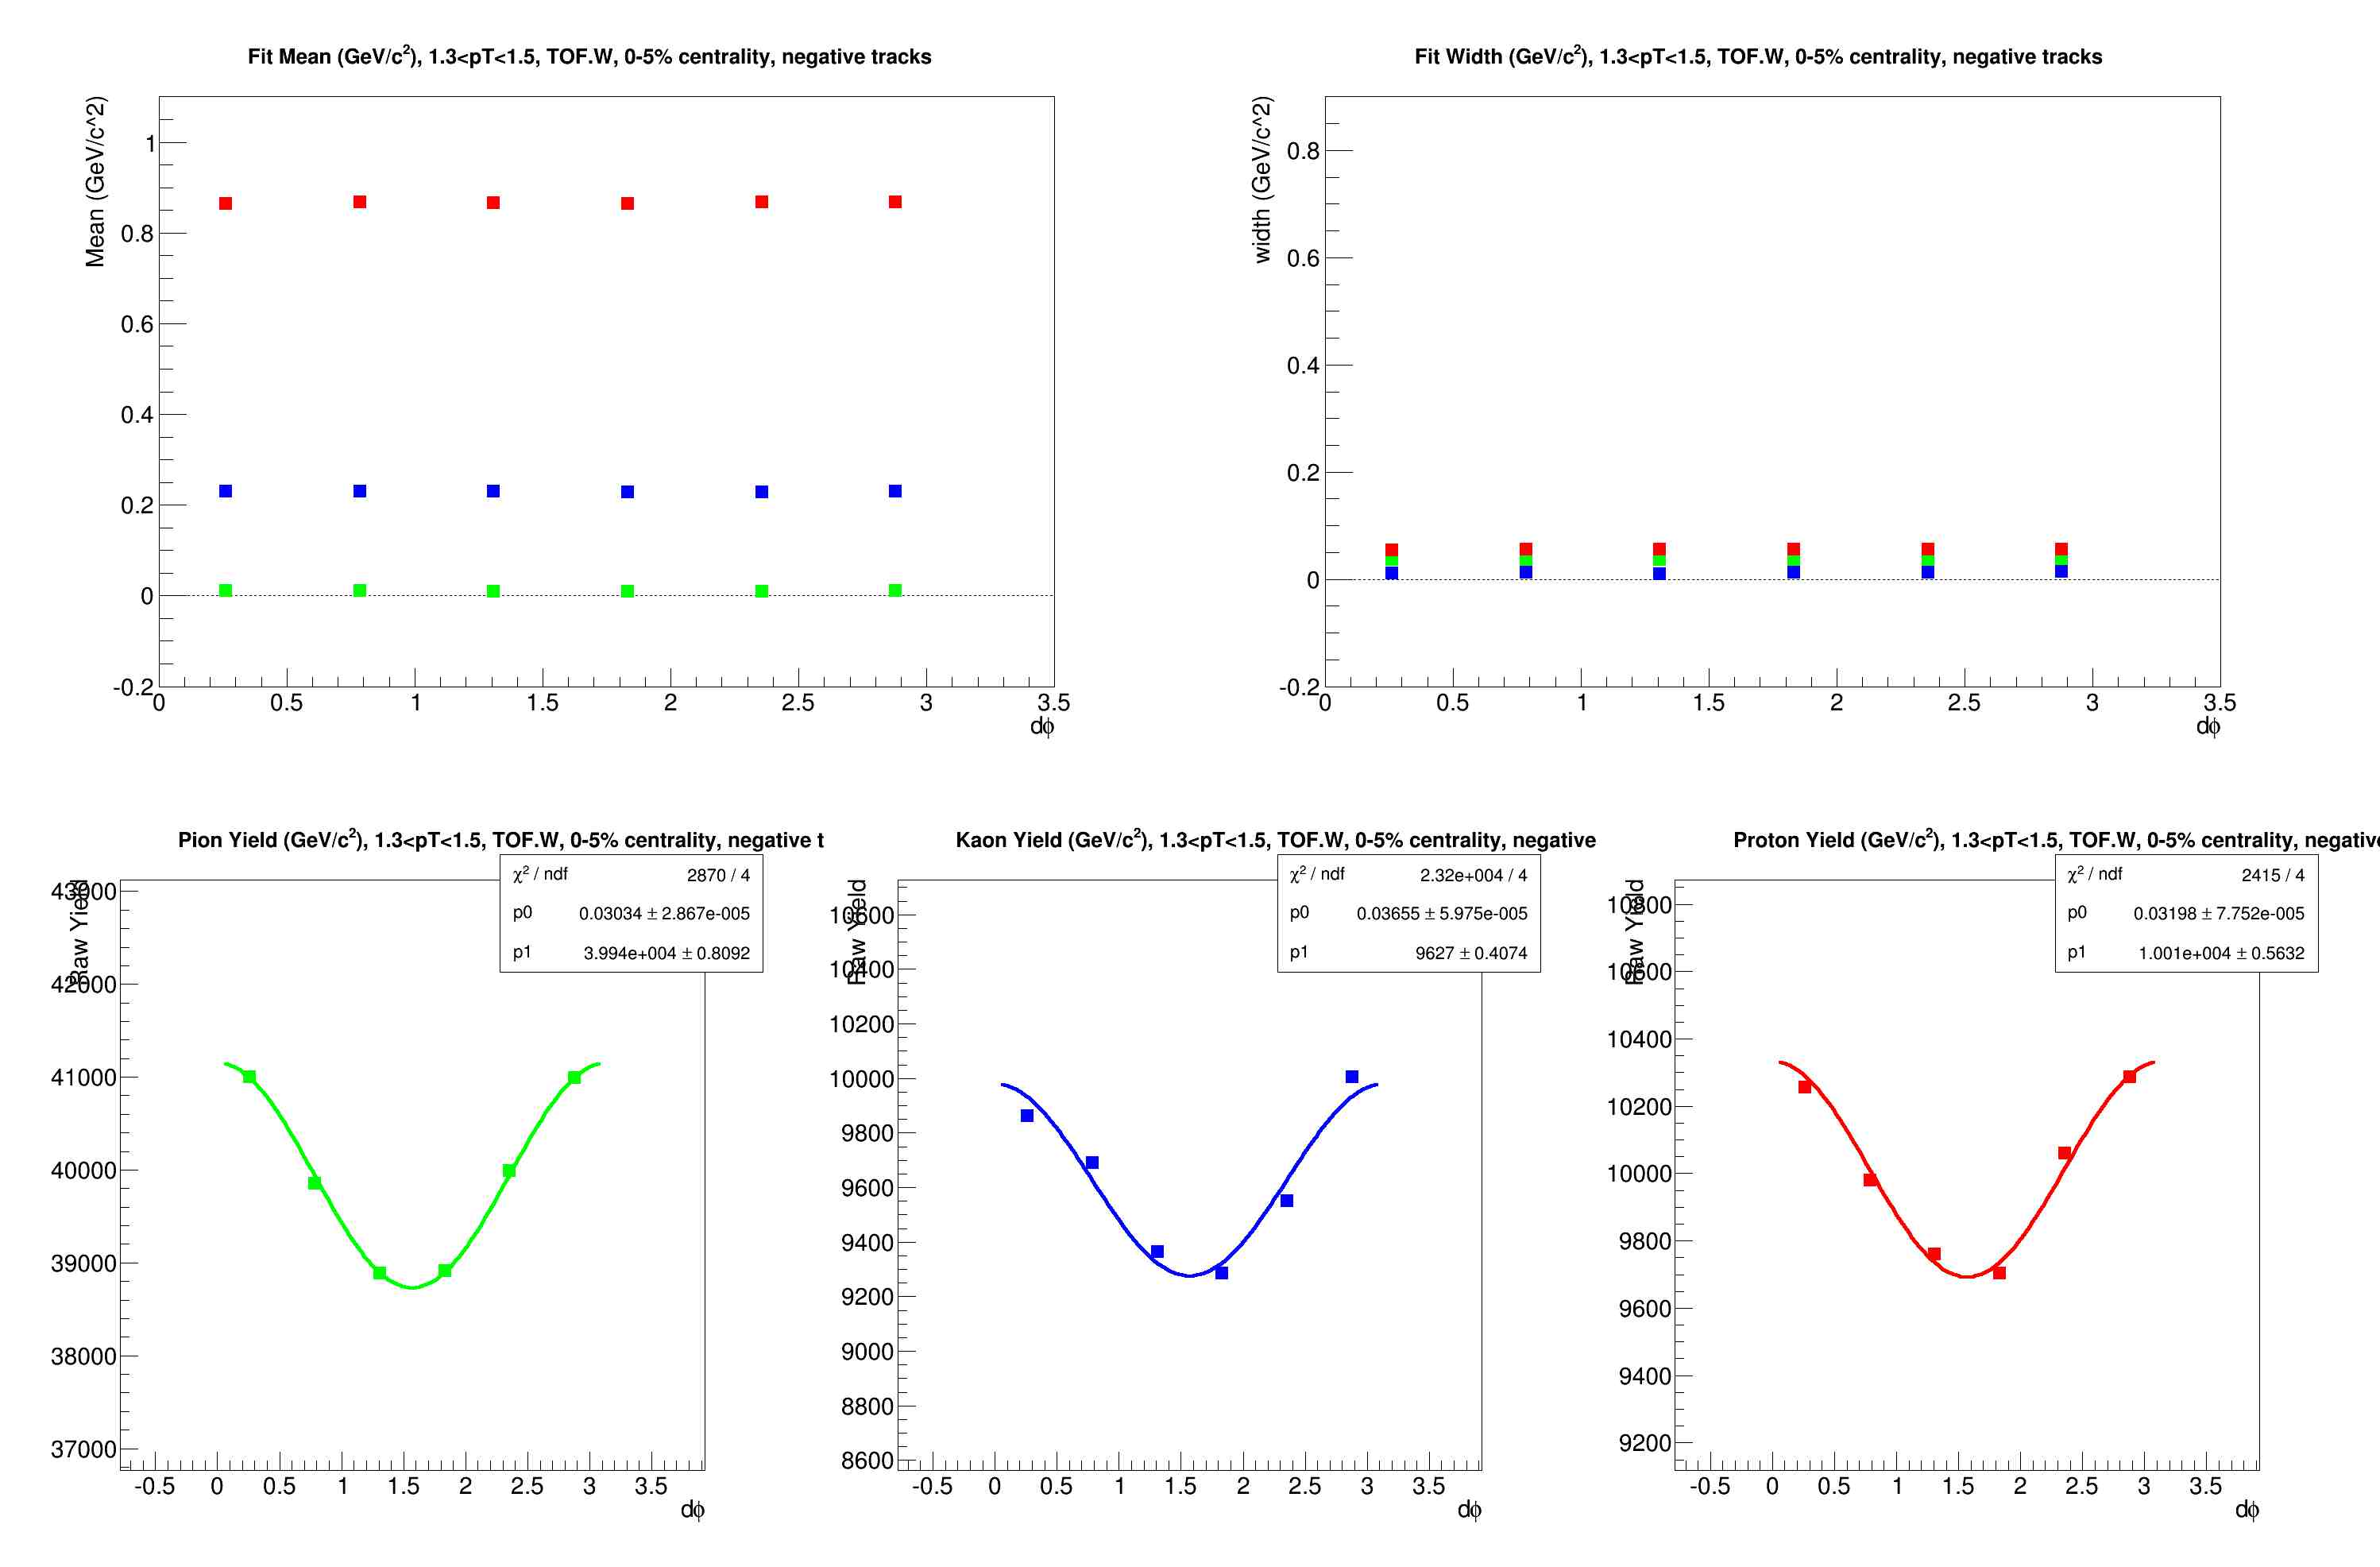
\includegraphics[width=1\textwidth]{lowptfits/fitParams_tof1_cent0_ch0_pT-13-15.jpg}
    \end{subfigure}
    \rule{35em}{0.5pt}
  \caption[PID fits and Yield vs $d\phi$ for $p_T$=1.3-1.5 GeV/c, TOF.W, negative particles ]{$m^2$ Gaussian fits for PID and resulting Yield vs $d\phi$ for $p_T$=1.3-1.5 GeV/c, TOF.W, negative particles}
  \label{fig:fits13-15neg}
\end{figure}

\begin{figure}[H]
  \centering
    \begin{subfigure}{1\textwidth}
    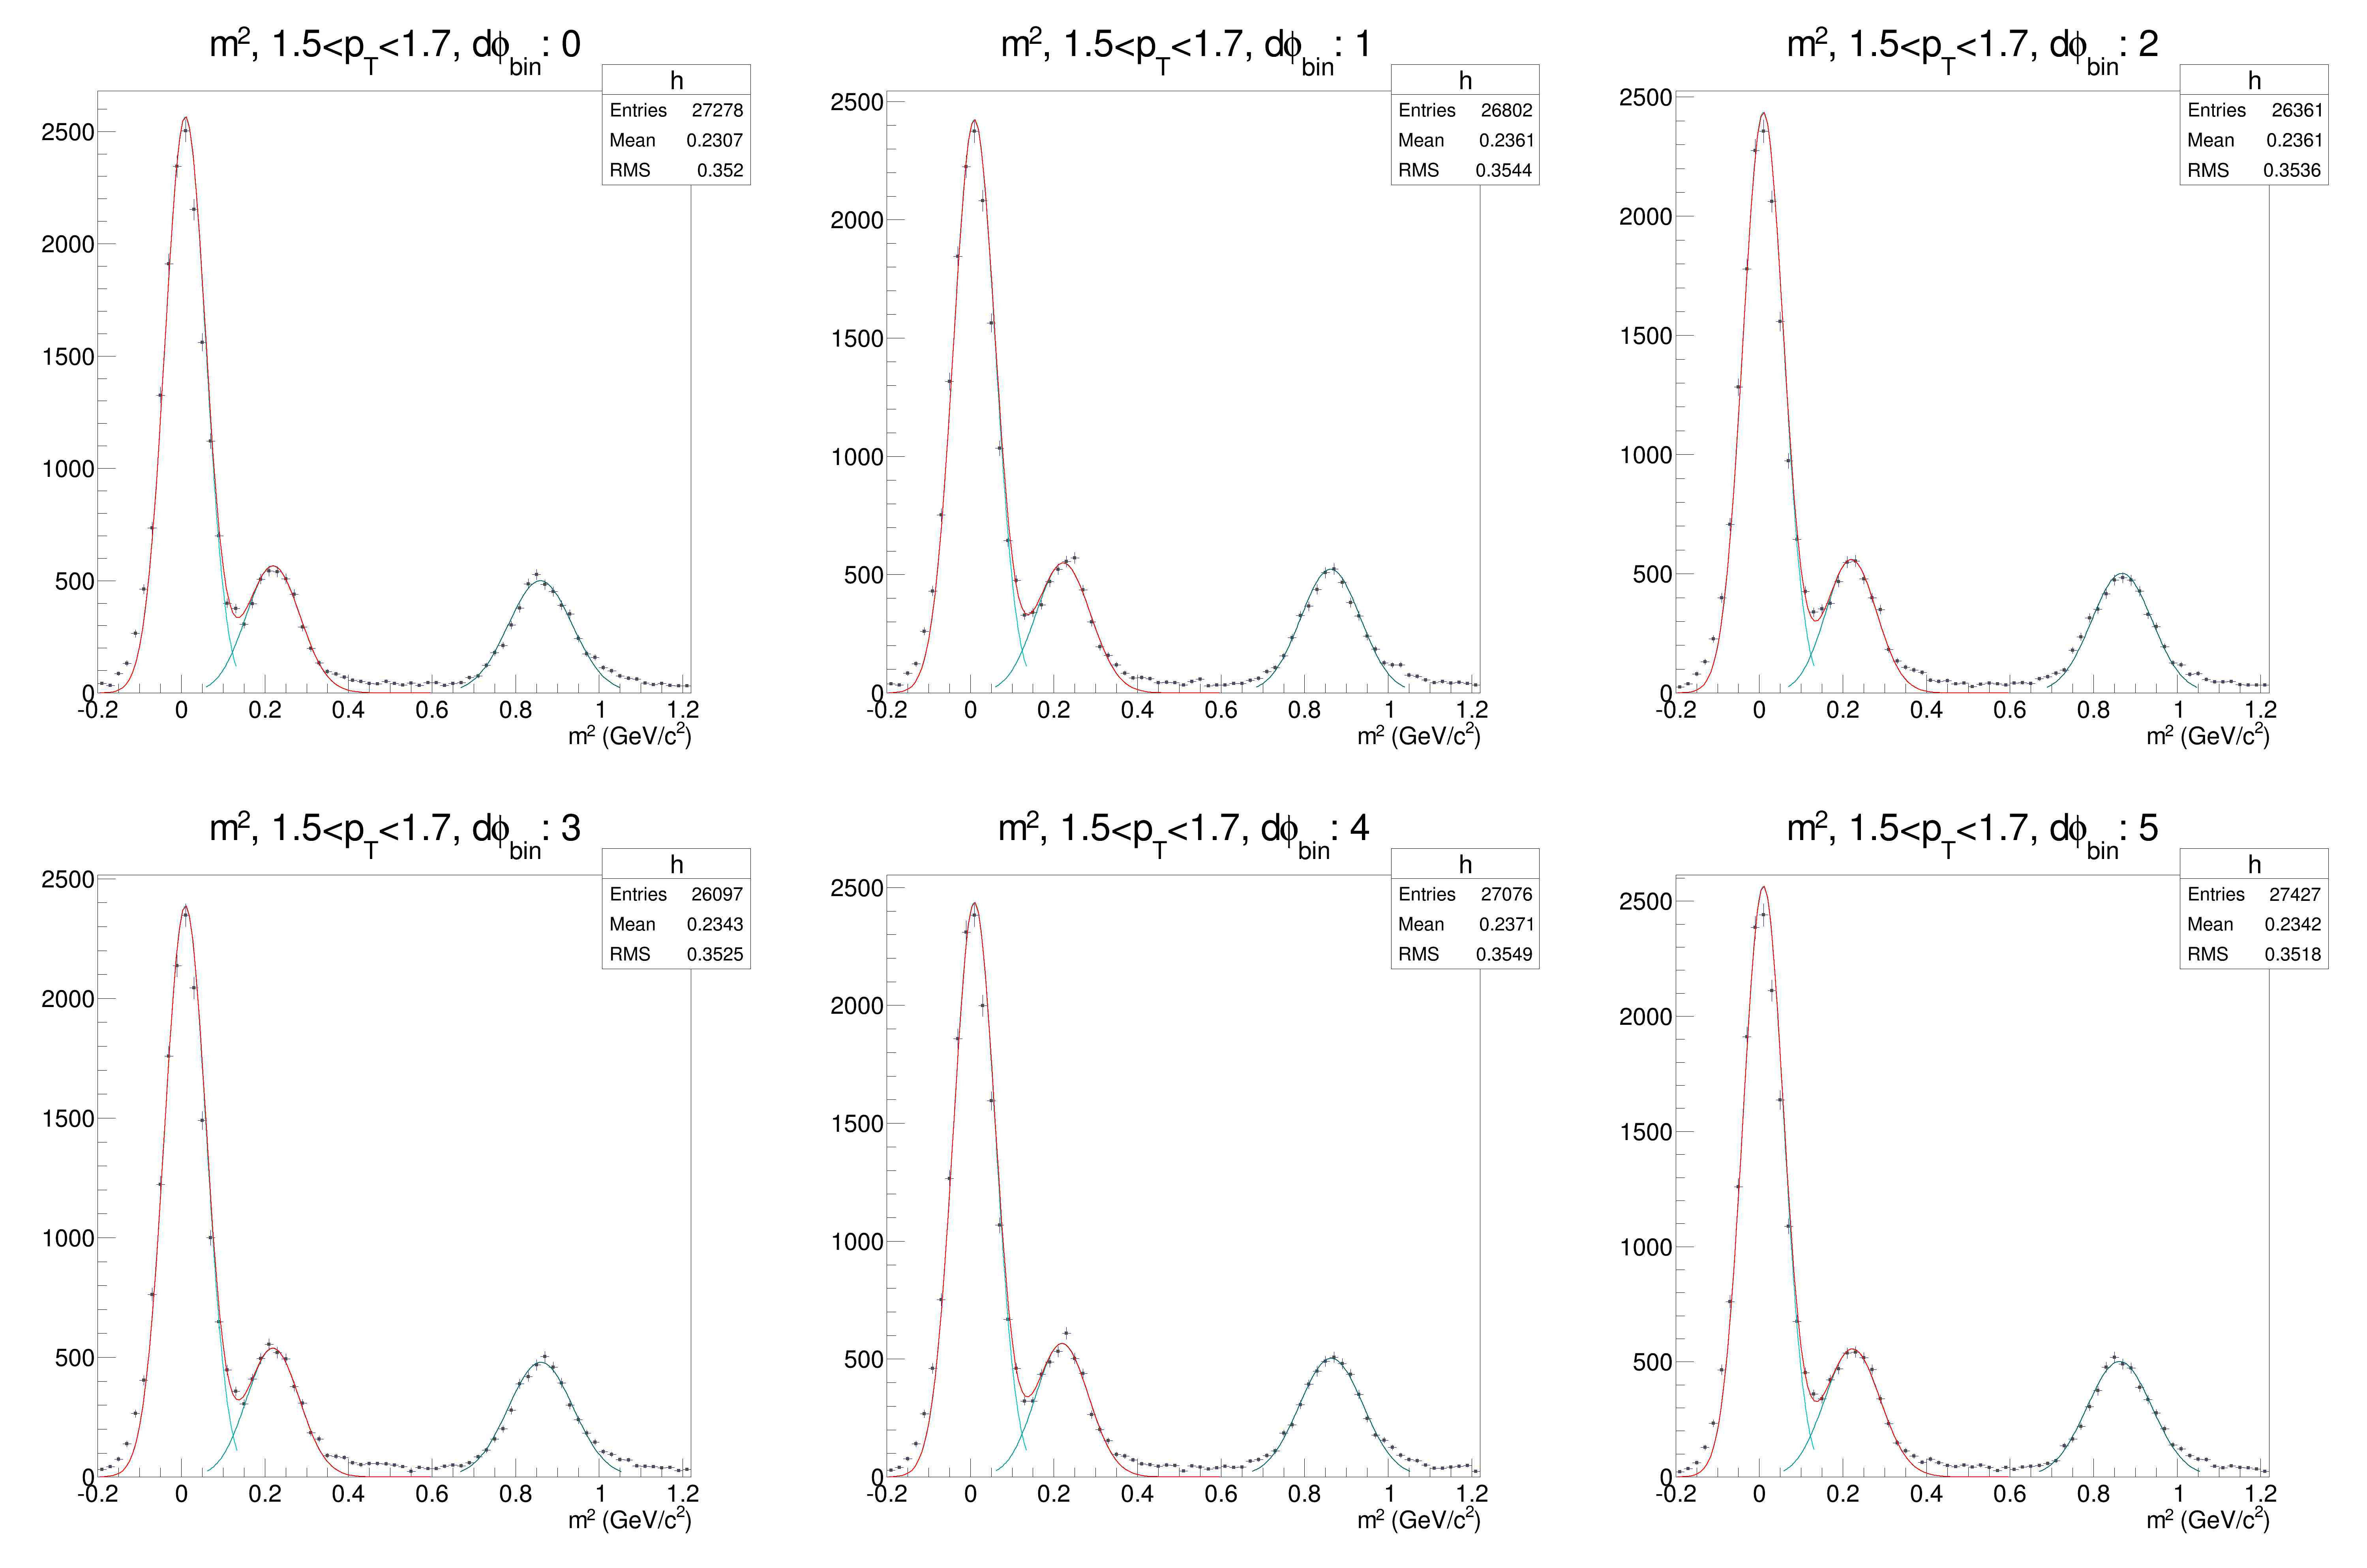
\includegraphics[width=1\textwidth]{lowptfits/yieldvsdphi_tof1_cent0_ch0_pT-15-17.jpg}
    \end{subfigure}
    \begin{subfigure}{1\textwidth}
    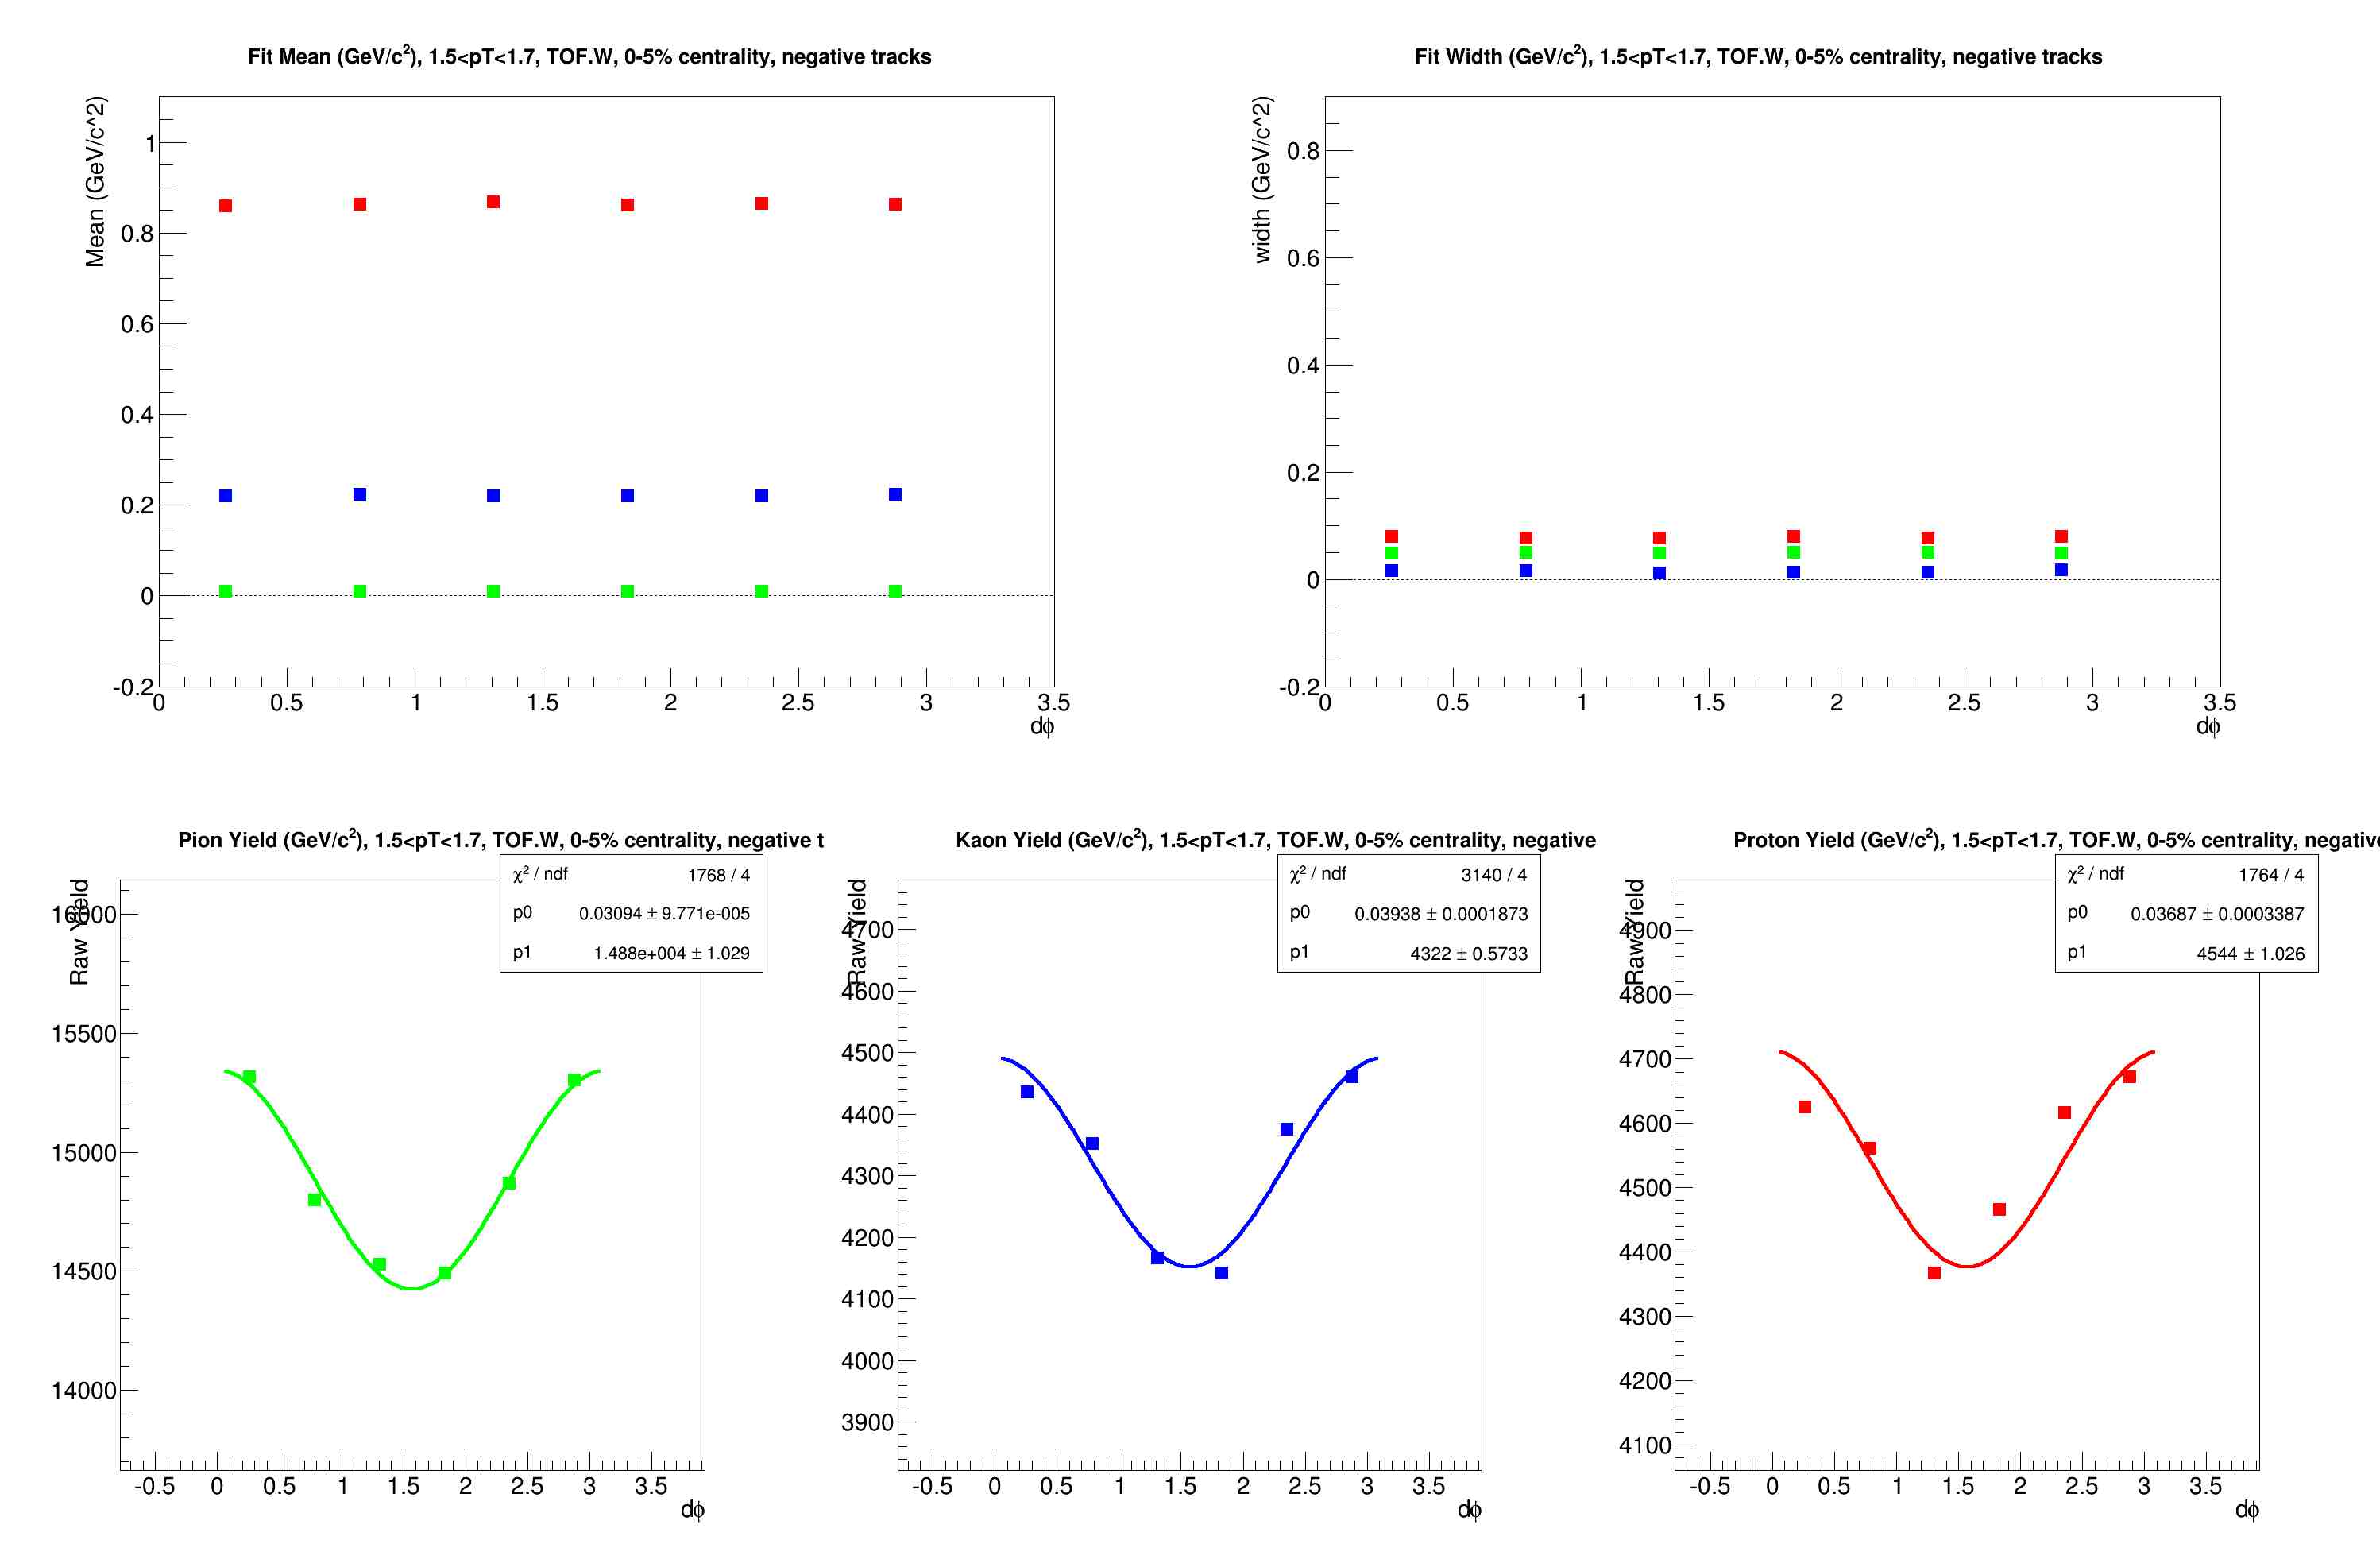
\includegraphics[width=1\textwidth]{lowptfits/fitParams_tof1_cent0_ch0_pT-15-17.jpg}
    \end{subfigure}
    \rule{35em}{0.5pt}
  \caption[PID fits and Yield vs $d\phi$ for $p_T$=1.5-1.7 GeV/c, TOF.W, negative particles ]{$m^2$ Gaussian fits for PID and resulting Yield vs $d\phi$ for $p_T$=1.5-1.7 GeV/c, TOF.W, negative particles}
  \label{fig:fits15-17neg}
\end{figure}

\begin{figure}[H]
  \centering
    \begin{subfigure}[p]{1\textwidth}
    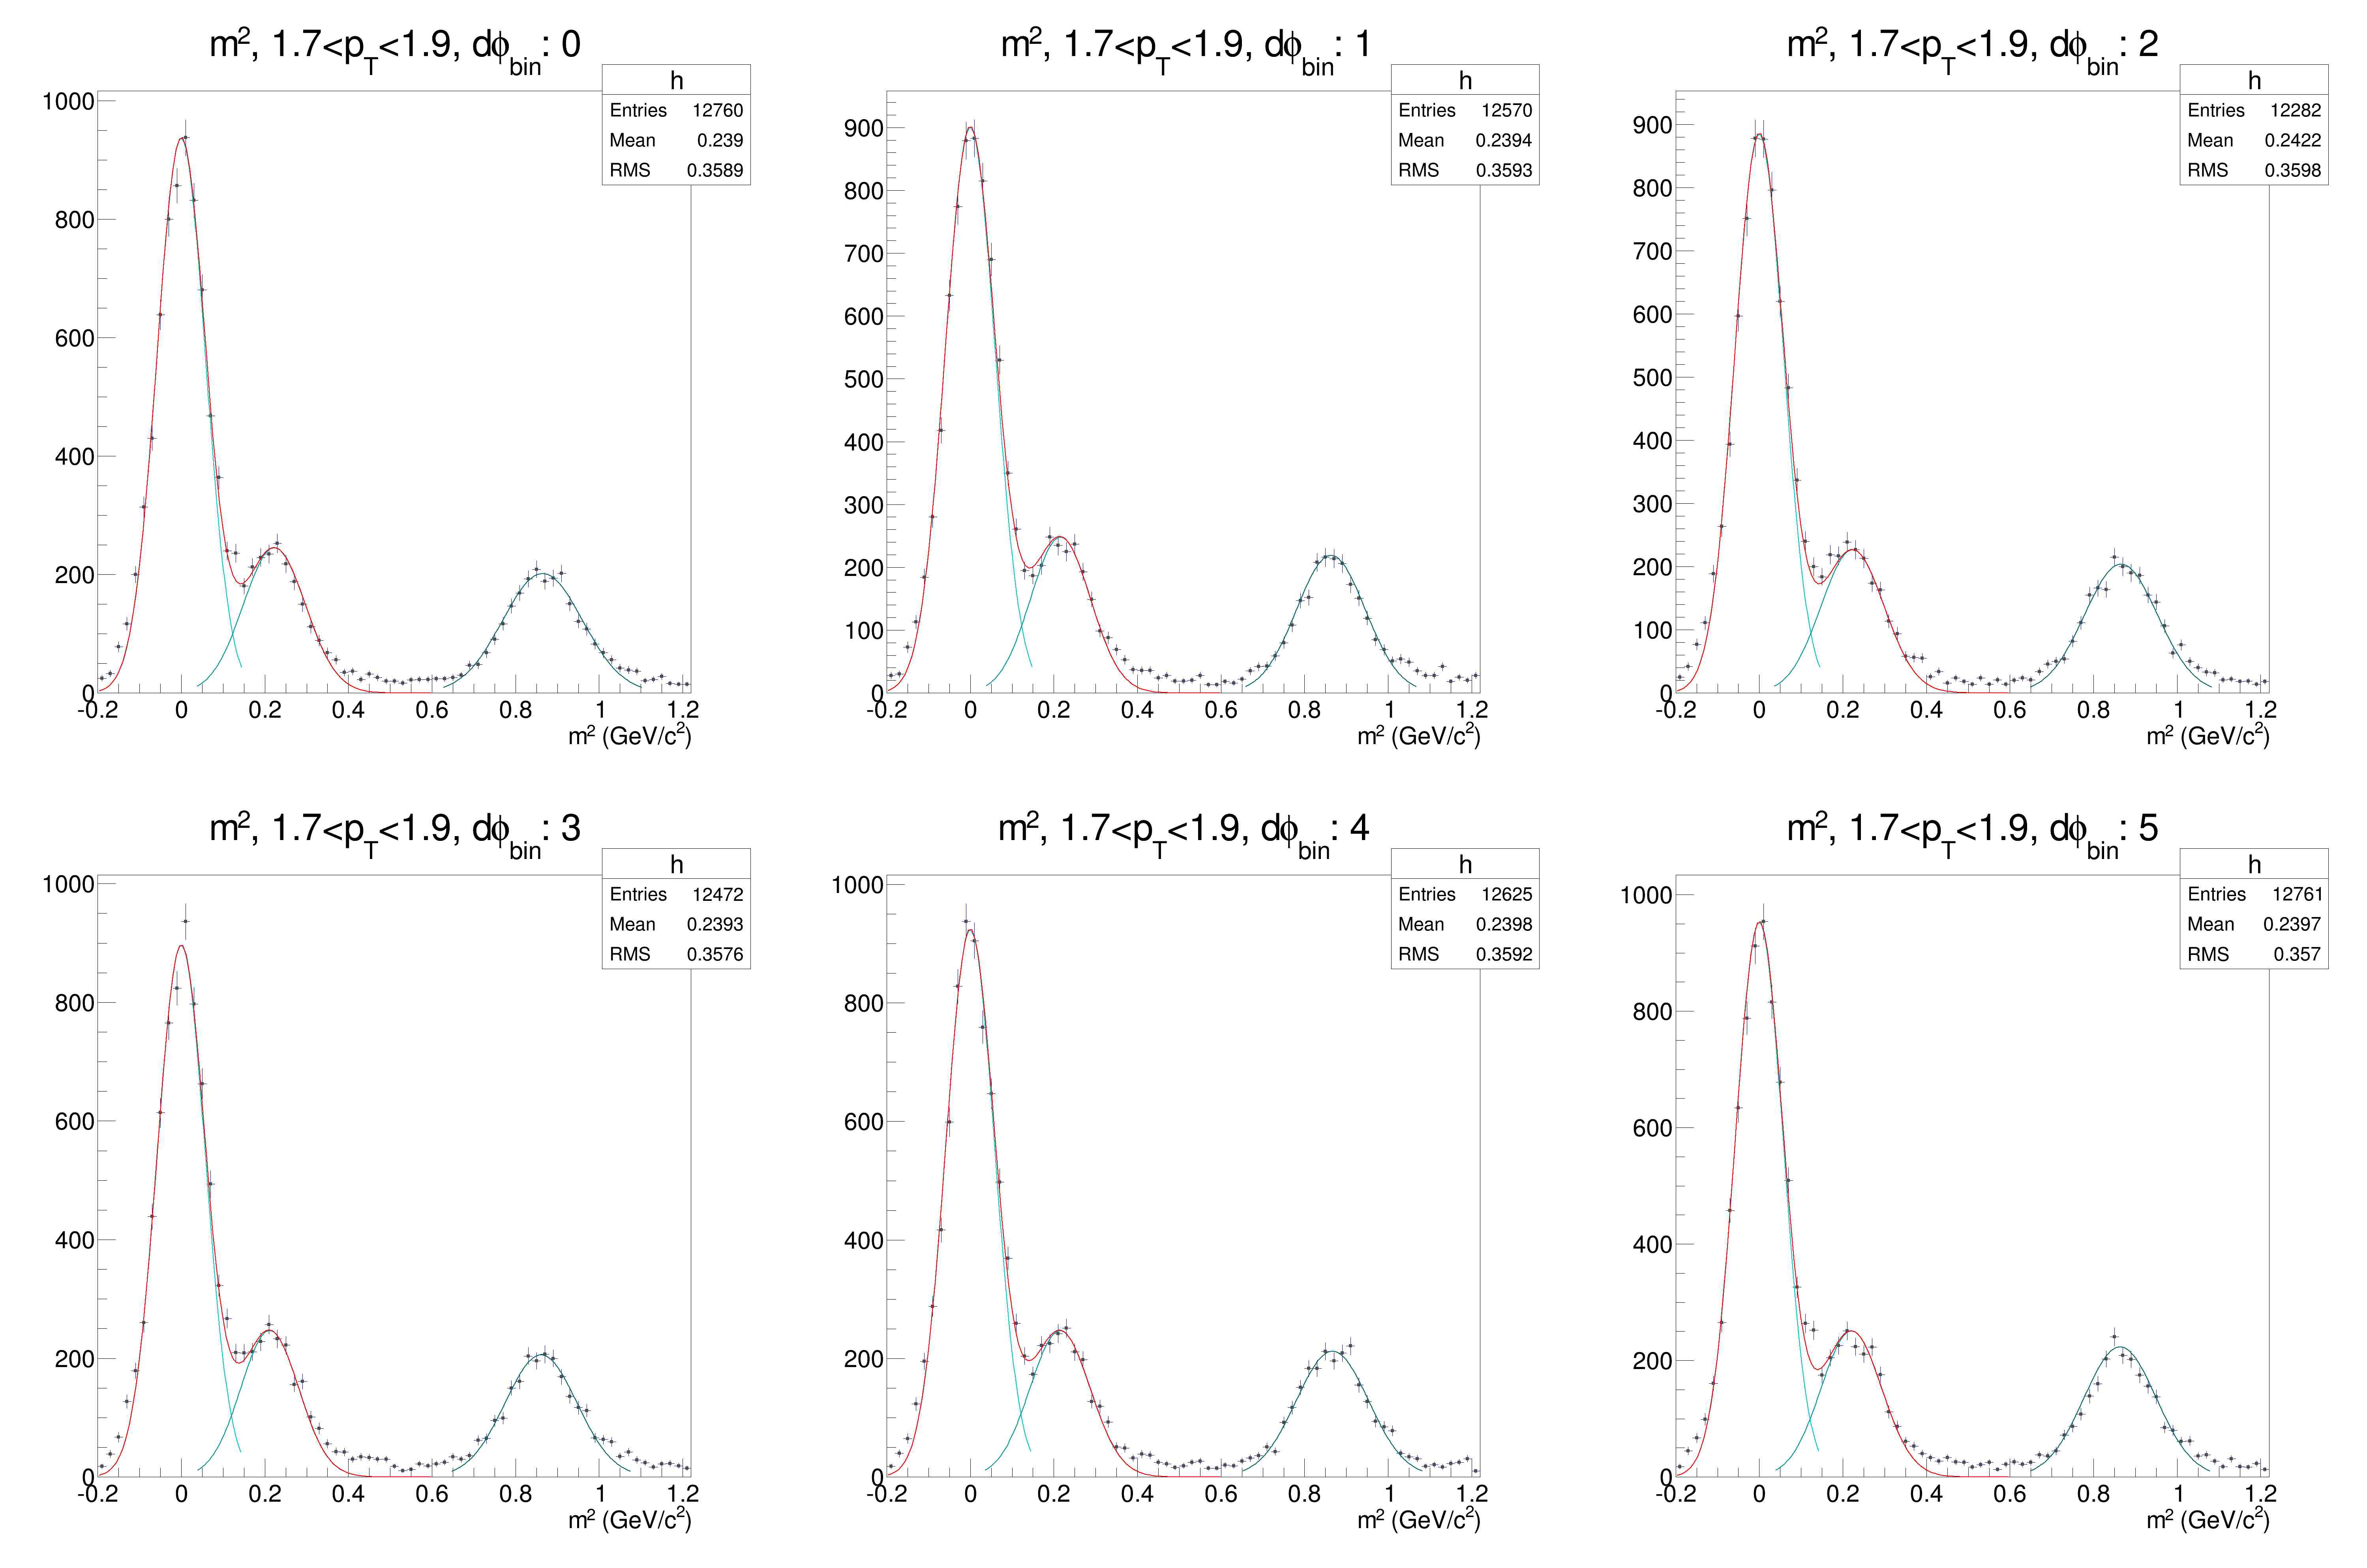
\includegraphics[width=1\textwidth]{lowptfits/yieldvsdphi_tof1_cent0_ch0_pT-17-19.jpg}
    \end{subfigure}
    \begin{subfigure}[p]{1\textwidth}
    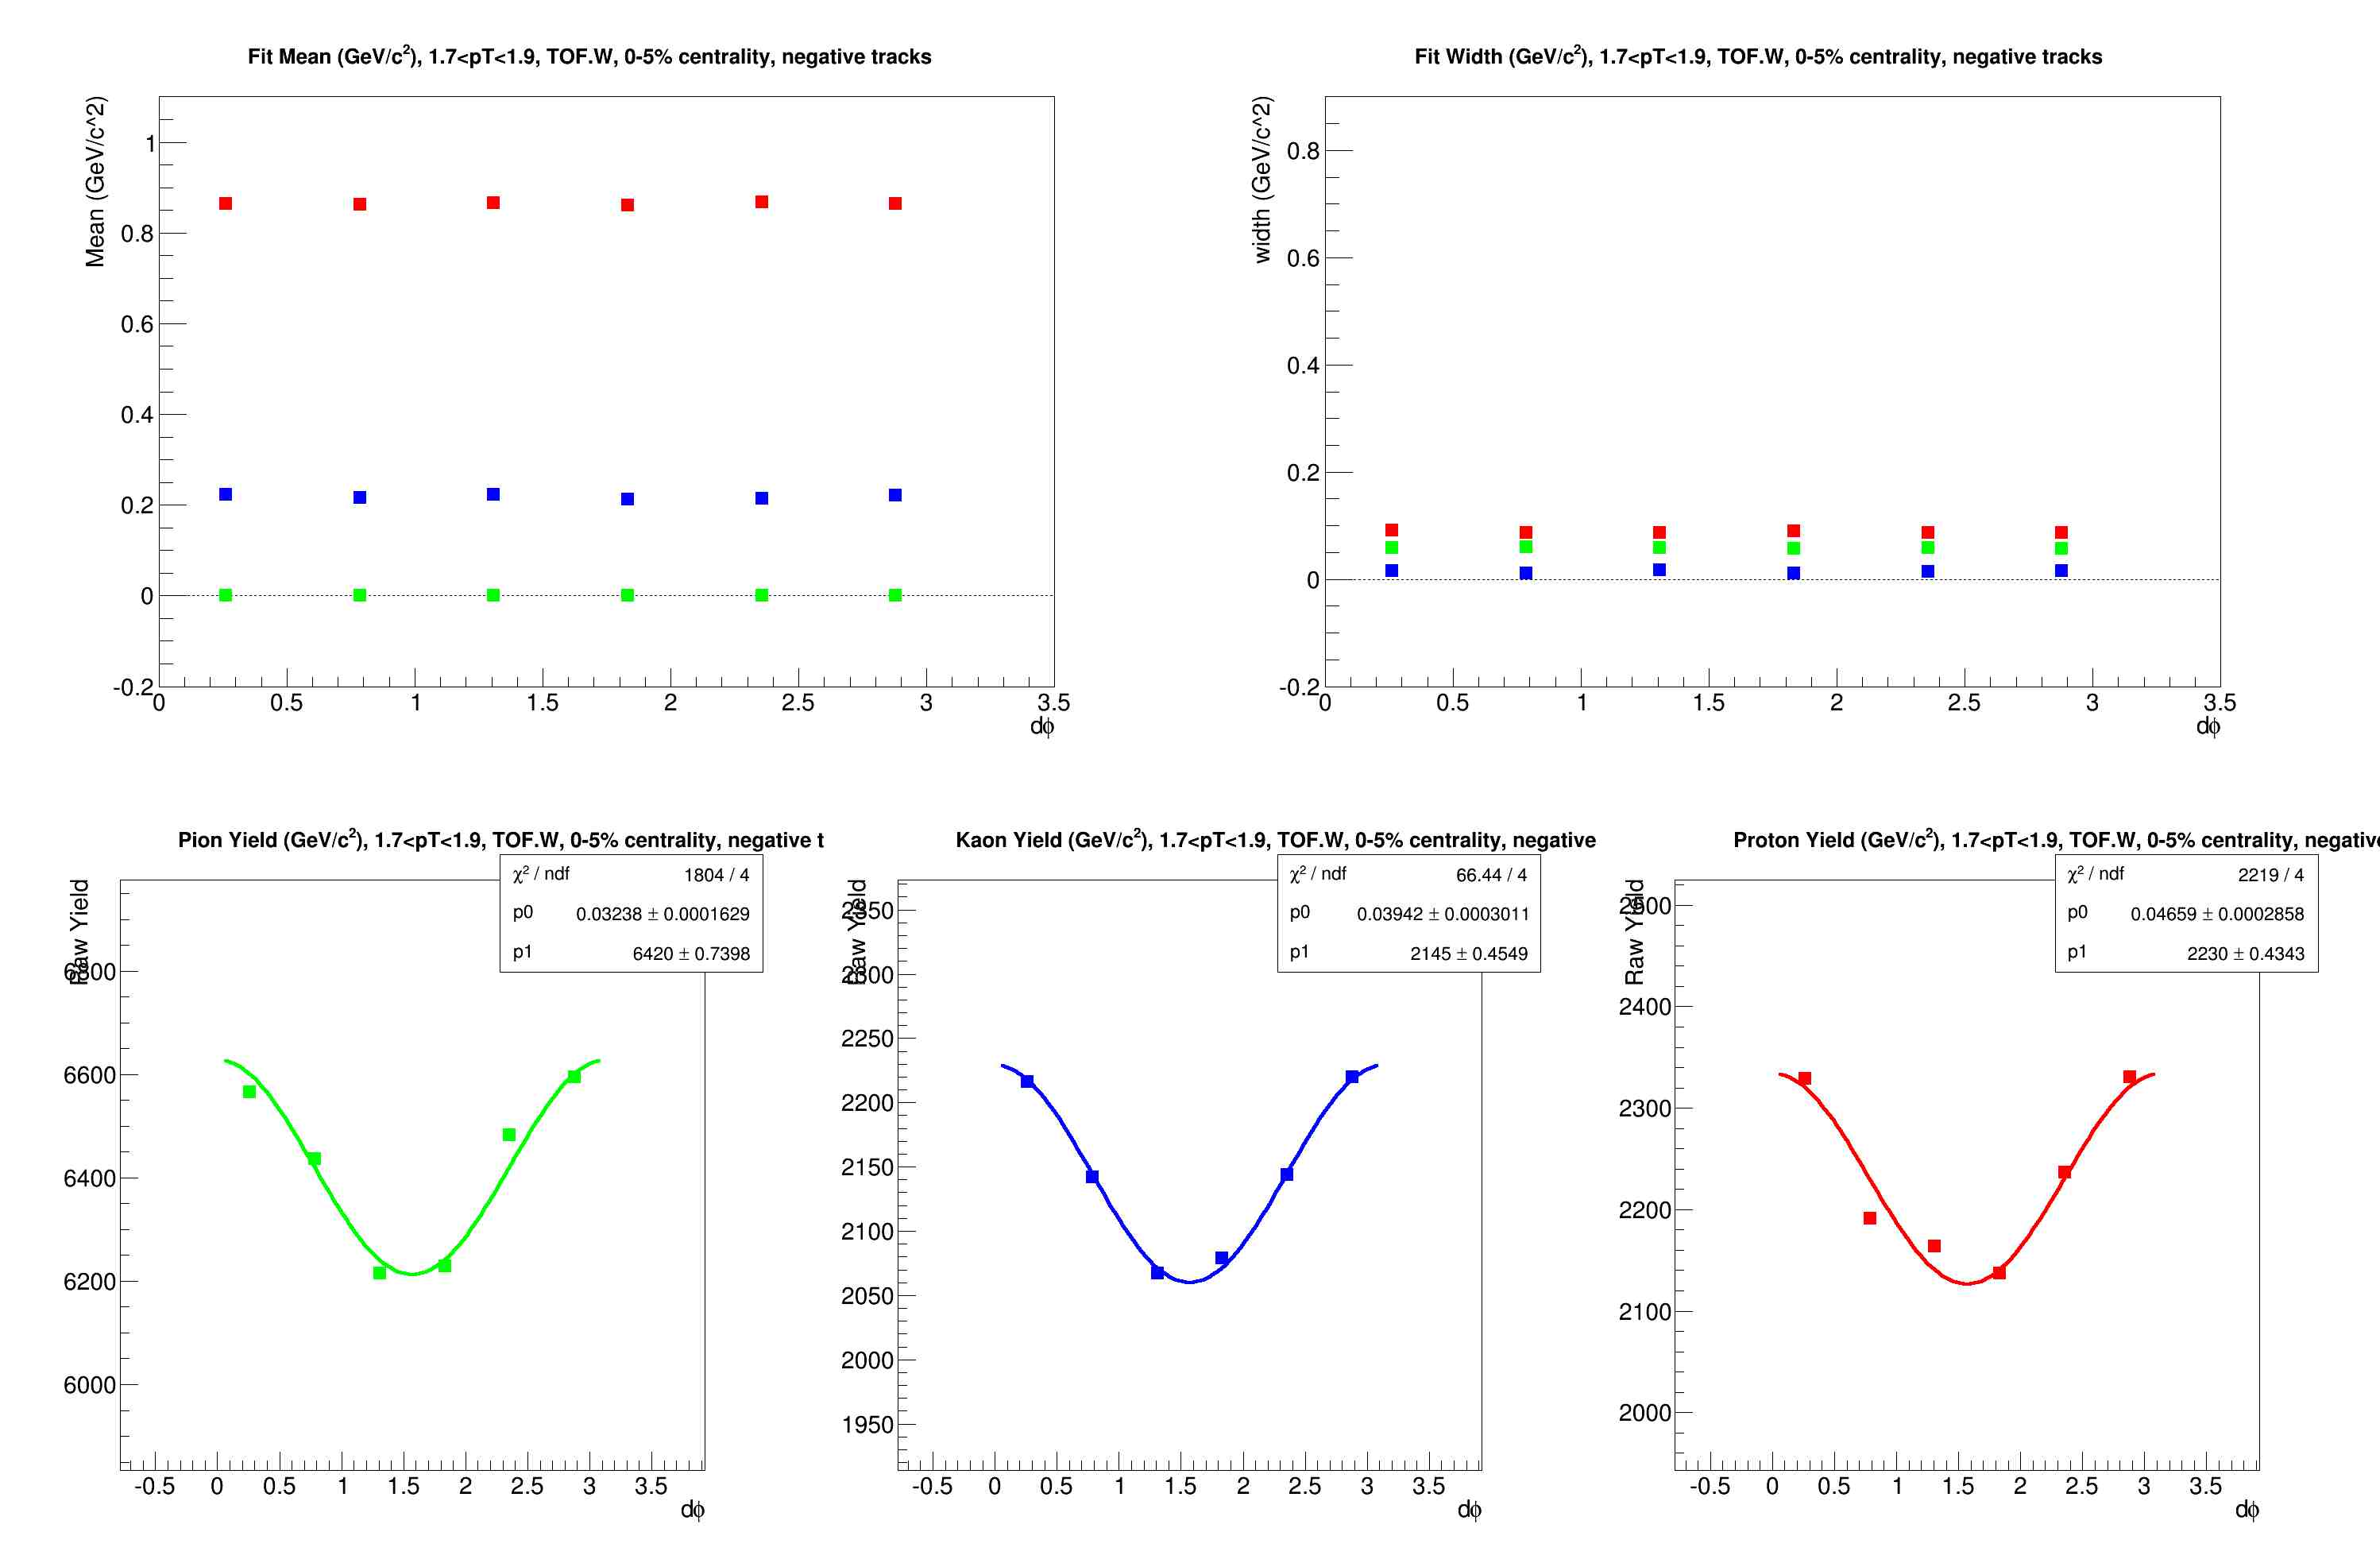
\includegraphics[width=1\textwidth]{lowptfits/fitParams_tof1_cent0_ch0_pT-17-19.jpg}
    \end{subfigure}
    \rule{35em}{0.5pt}
  \caption[PID fits and Yield vs $d\phi$ for $p_T$=1.7-1.9 GeV/c, TOF.W, negative particles ]{$m^2$ Gaussian fits for PID and resulting Yield vs $d\phi$ for $p_T$=1.7-1.9 GeV/c, TOF.W, negative particles}
  \label{fig:fits17-19neg}
\end{figure}

\begin{figure}[H]
  \centering
    \begin{subfigure}[p]{1\textwidth}
    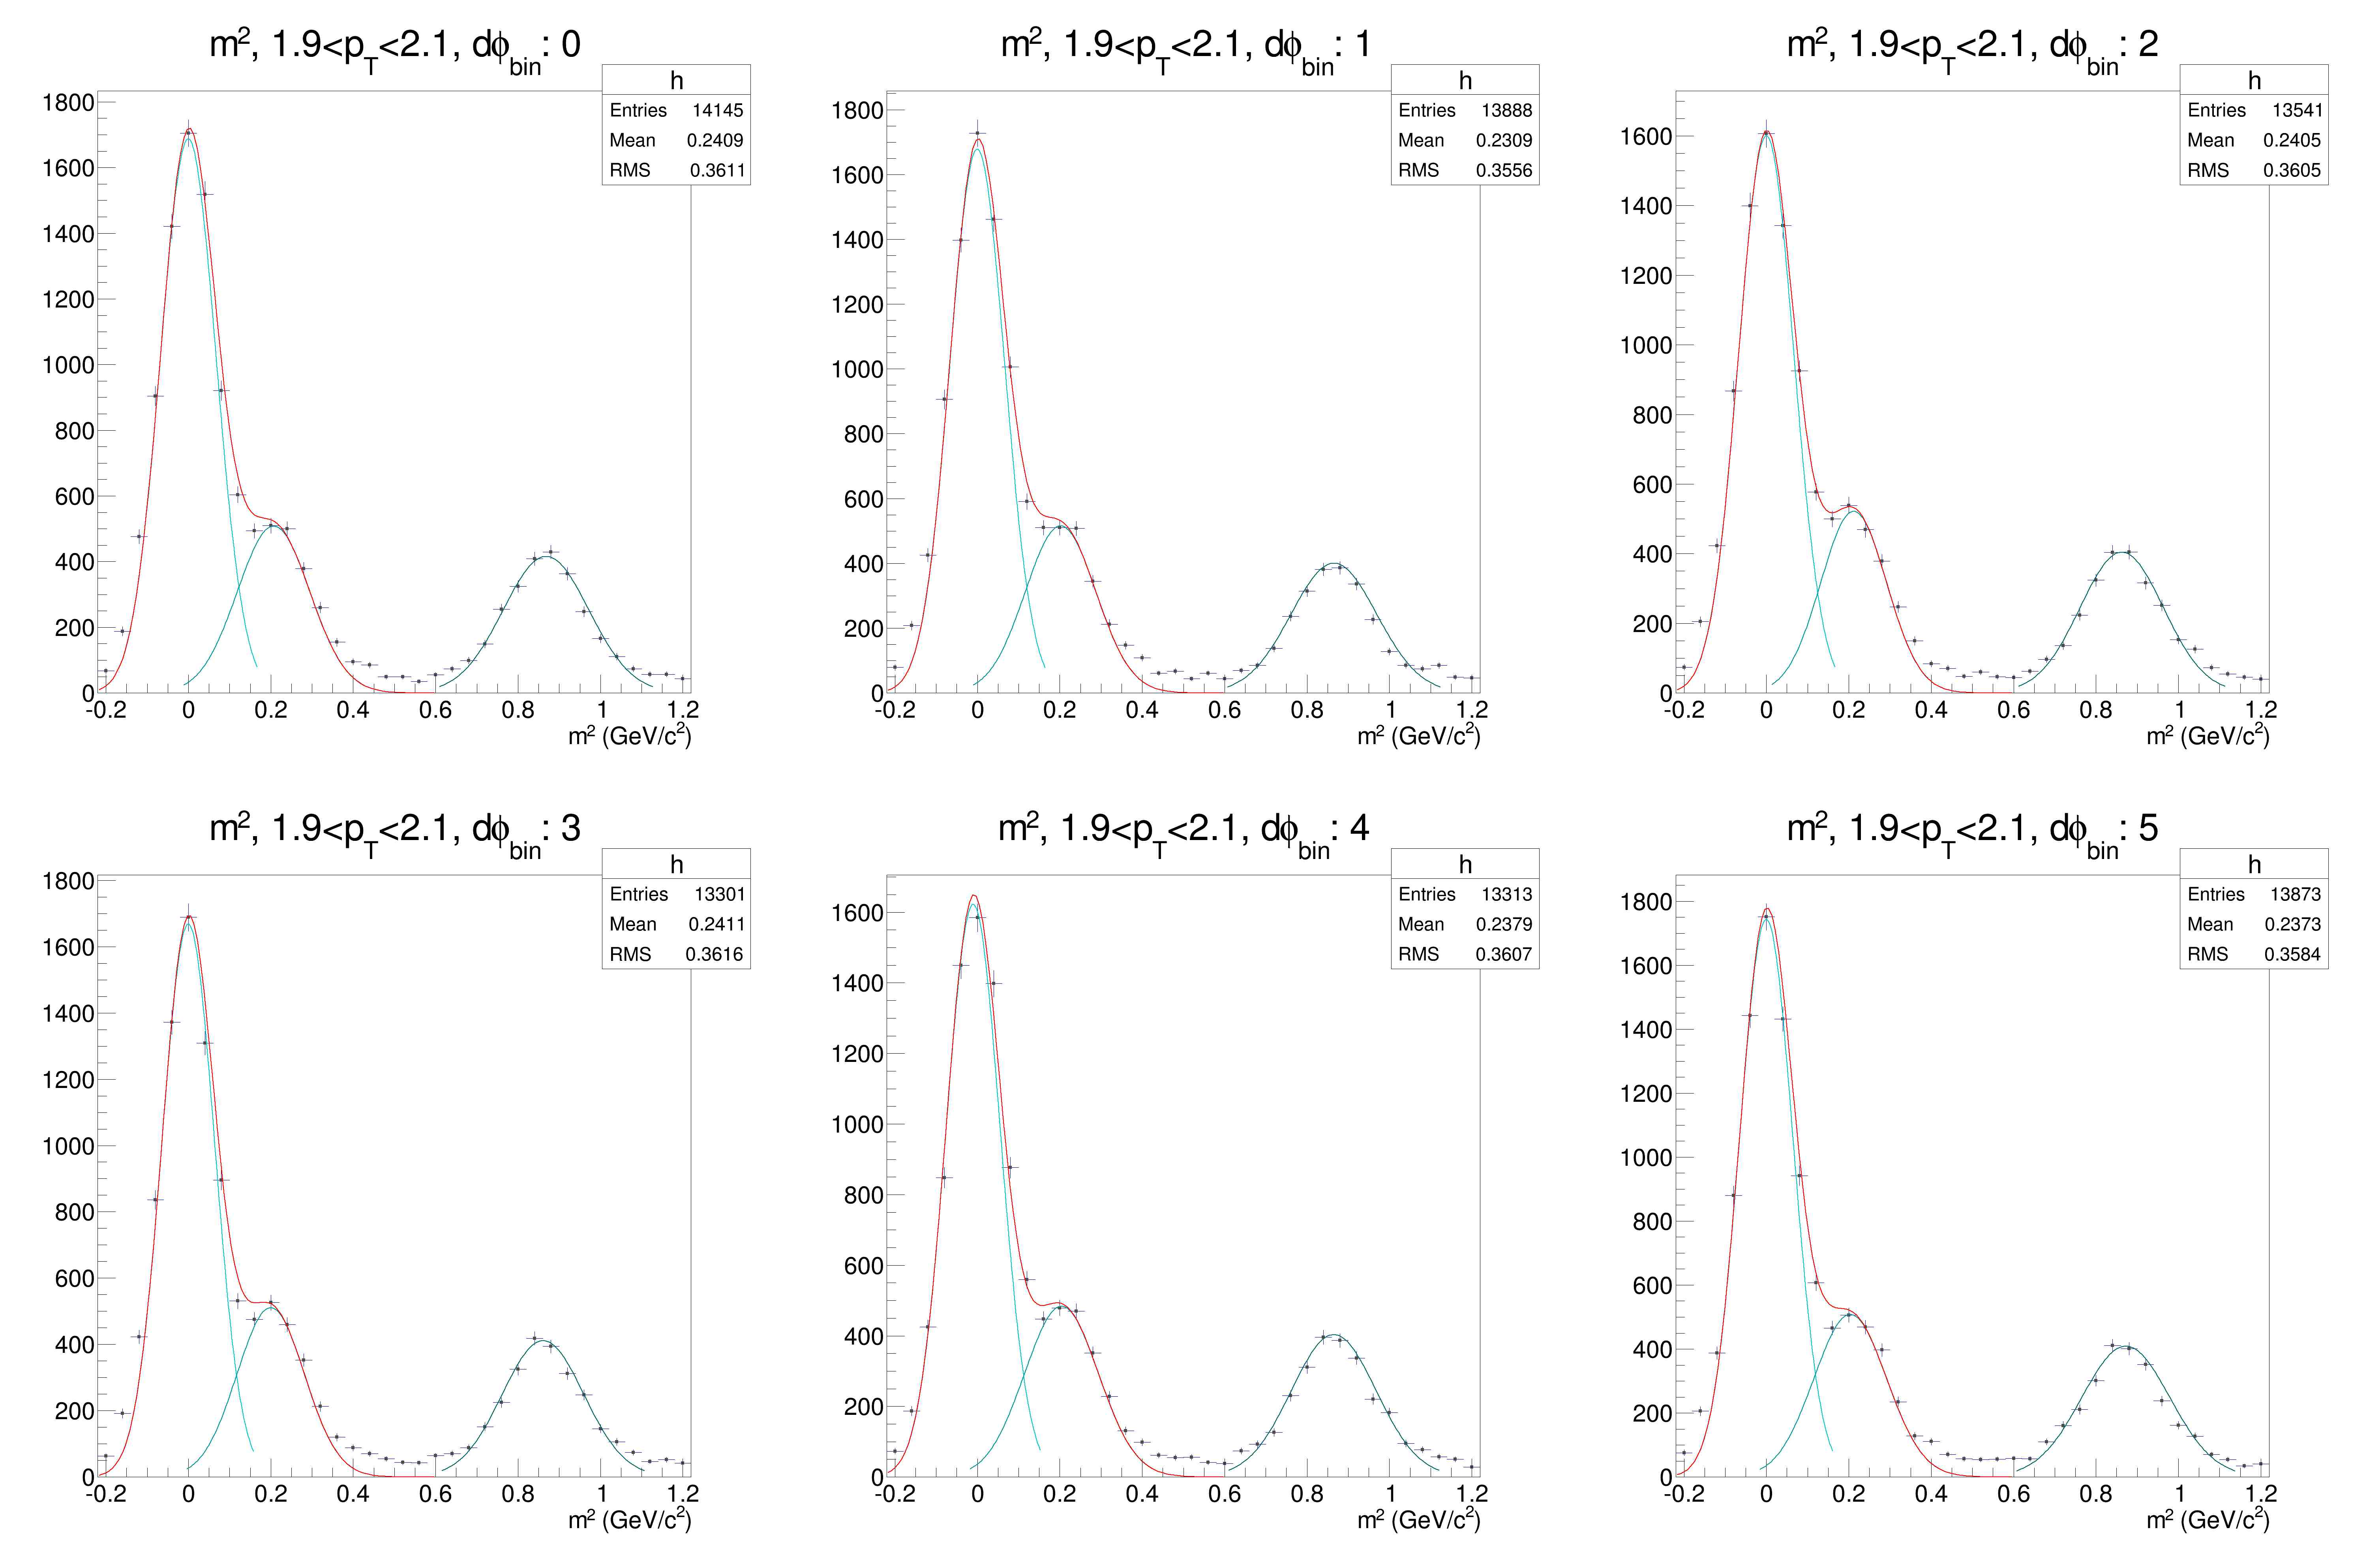
\includegraphics[width=1\textwidth]{lowptfits/yieldvsdphi_tof1_cent0_ch0_pT-19-21.jpg}
    \end{subfigure}
    \begin{subfigure}[p]{1\textwidth}
    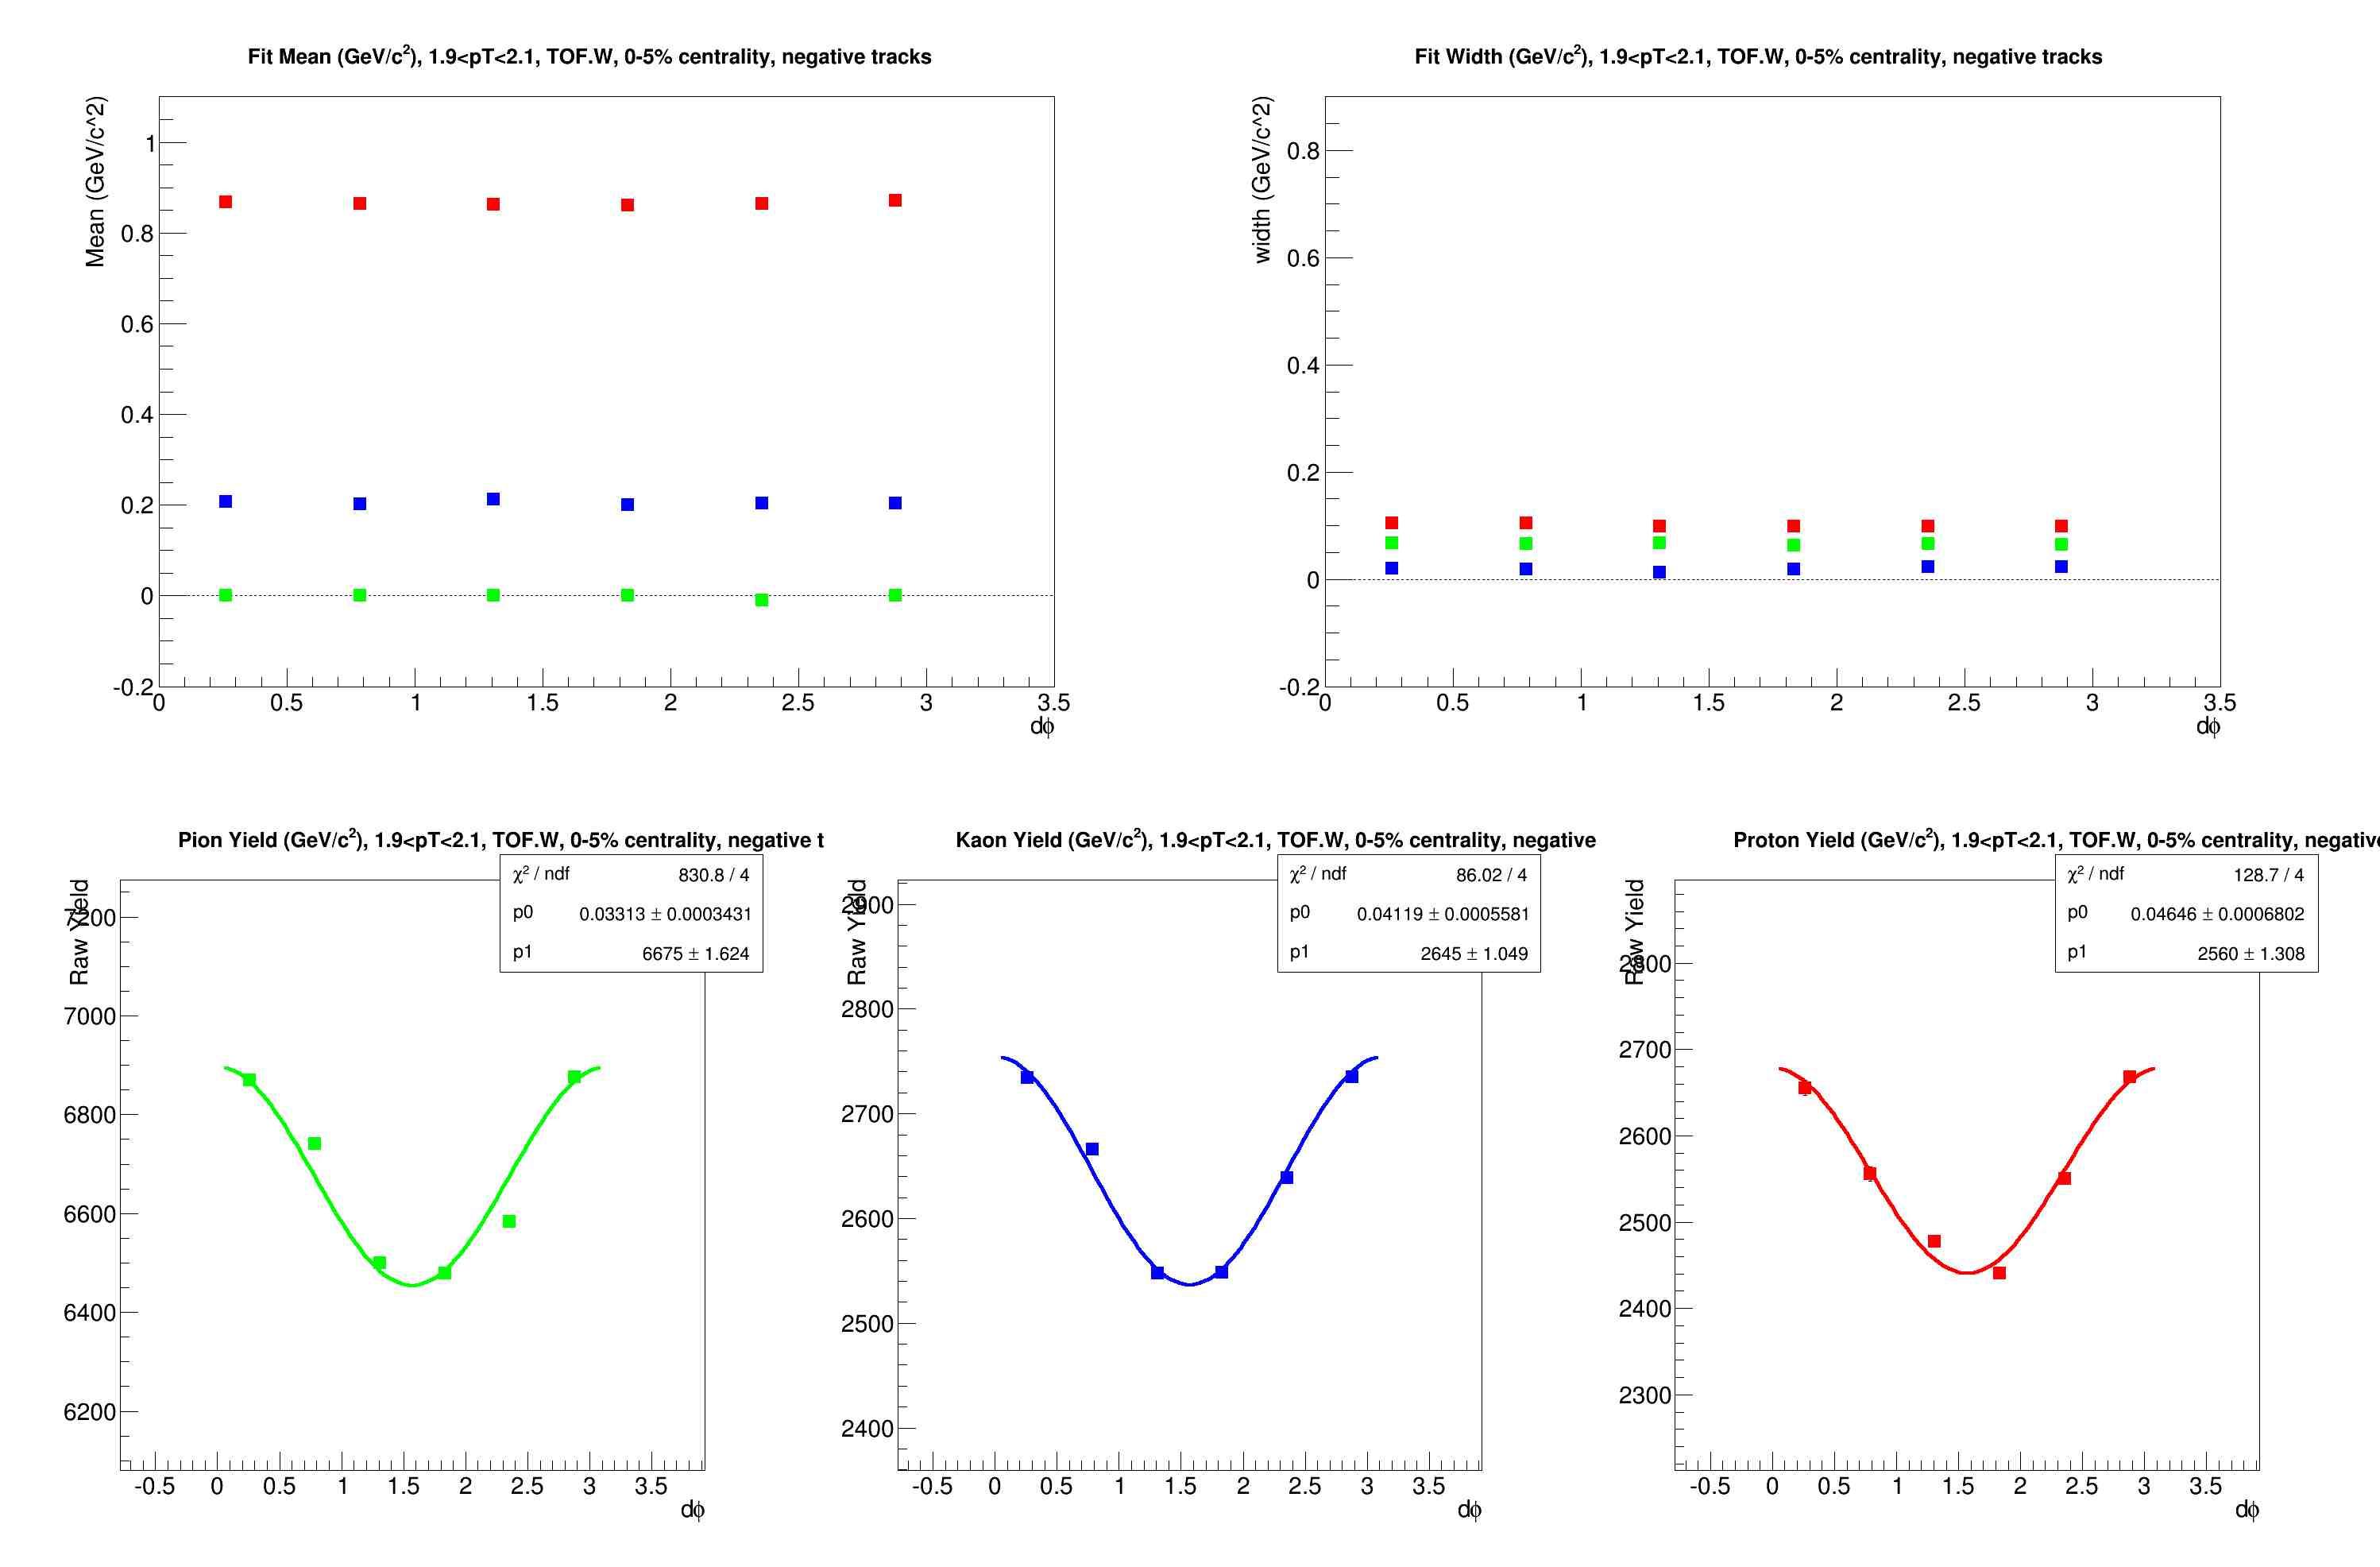
\includegraphics[width=1\textwidth]{lowptfits/fitParams_tof1_cent0_ch0_pT-19-21.jpg}
    \end{subfigure}
    \rule{35em}{0.5pt}
  \caption[PID fits and Yield vs $d\phi$ for $p_T$=1.9-2.1 GeV/c, TOF.W, negative particles ]{$m^2$ Gaussian fits for PID and resulting Yield vs $d\phi$ for $p_T$=1.9-2.1 GeV/c, TOF.W, negative particles}
  \label{fig:fits19-21neg}
\end{figure}

\subsubsection{Mixed Gaussian fits, $p_T$=1.3-2.1 GeV/c, TOF.W, positive charged tracks}

\begin{figure}[H]
  \centering
    \begin{subfigure}[p]{1\textwidth}
    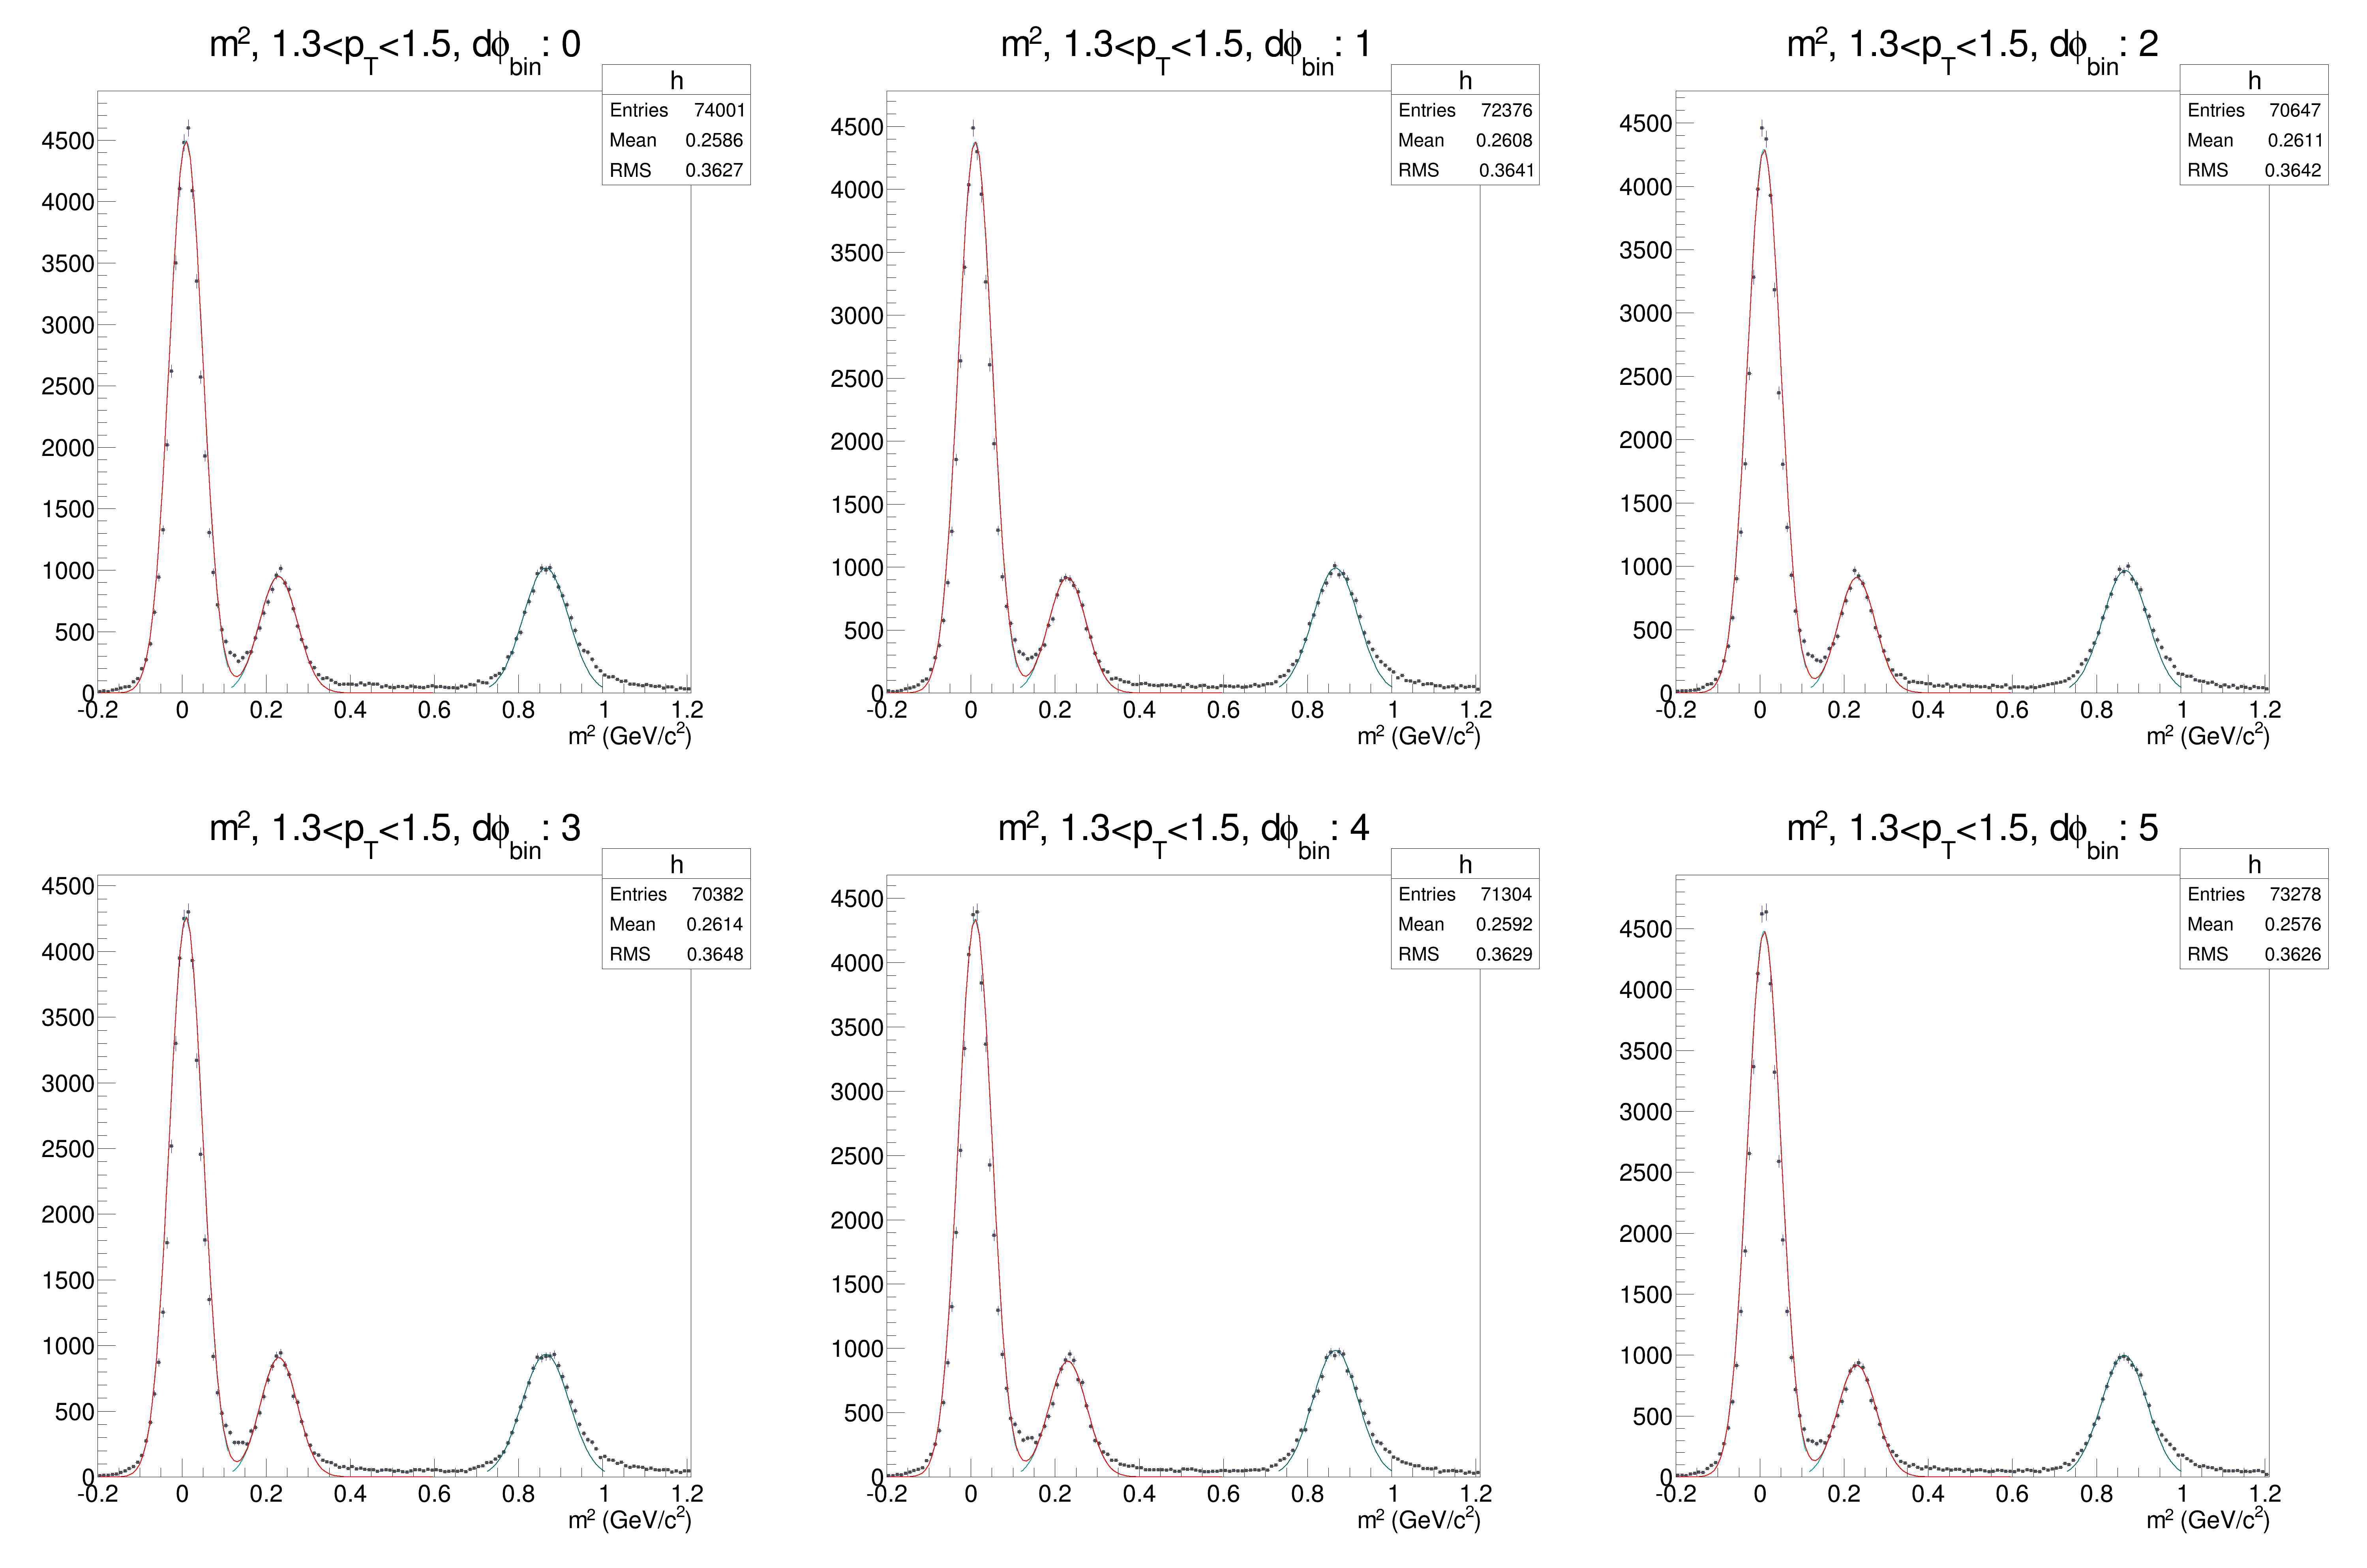
\includegraphics[width=1\textwidth]{lowptfits/yieldvsdphi_tof1_cent0_ch1_pT-13-15.jpg}
    \end{subfigure}
    \begin{subfigure}[p]{1\textwidth}
    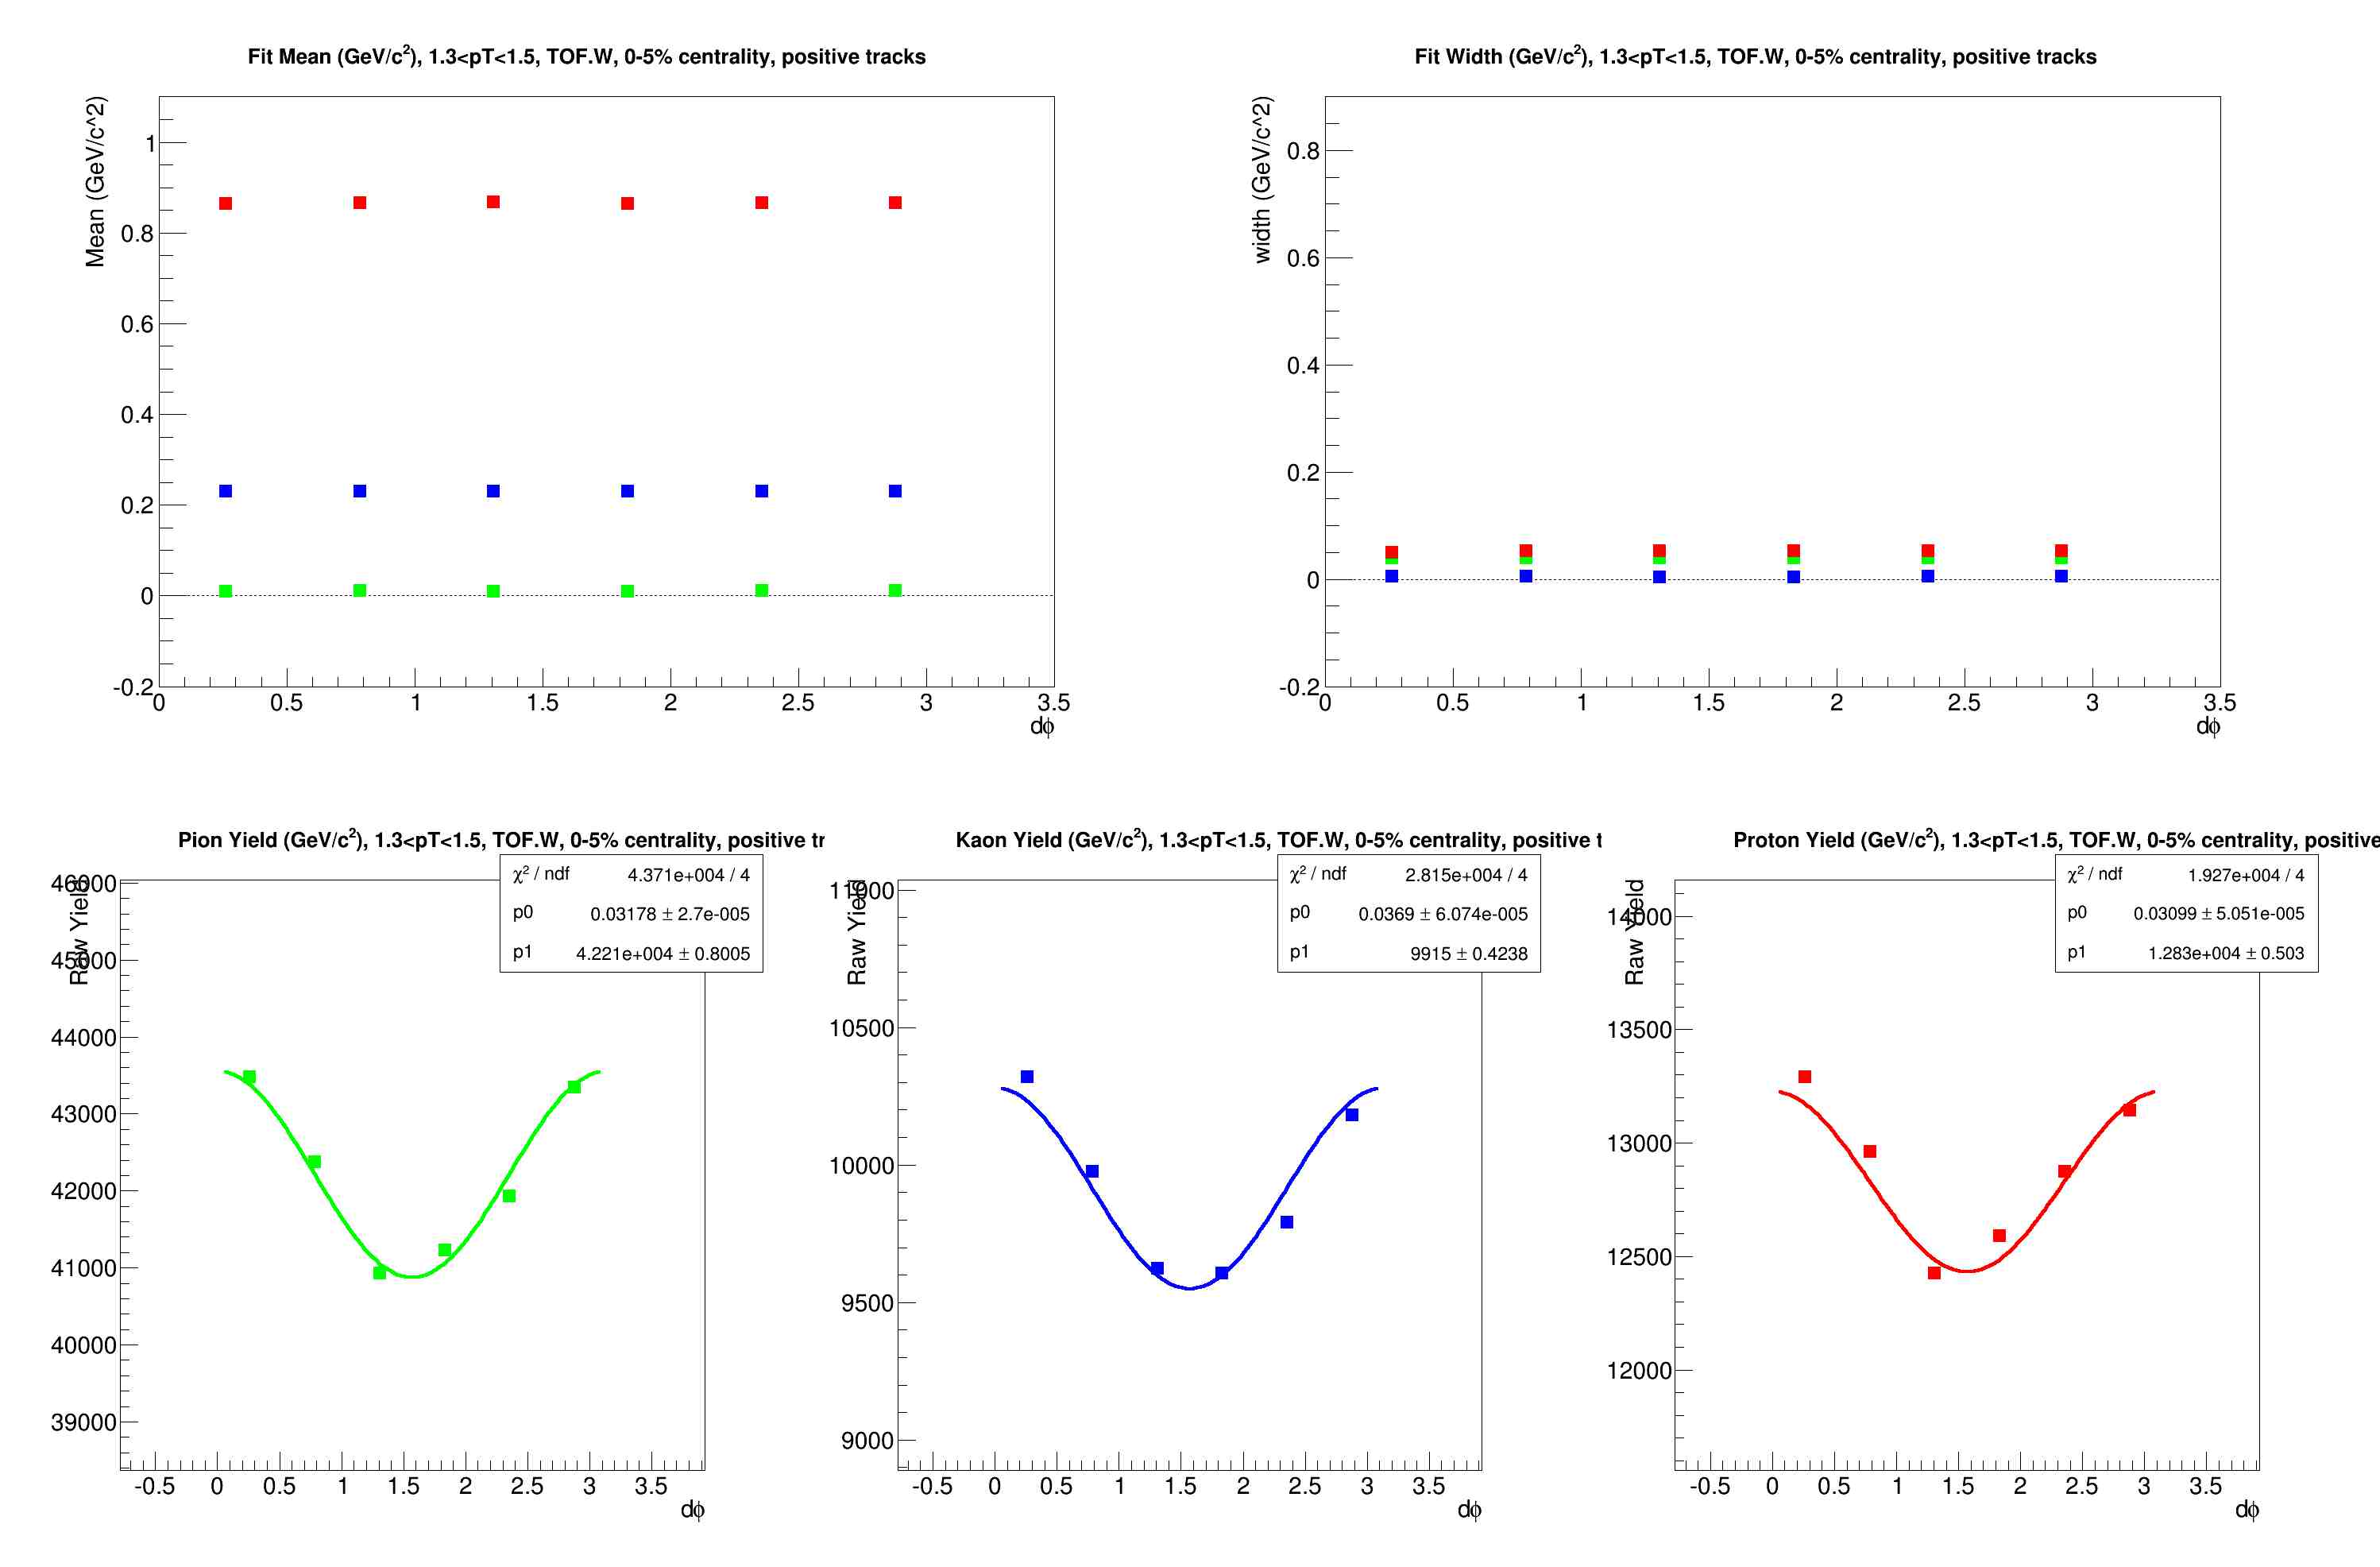
\includegraphics[width=1\textwidth]{lowptfits/fitParams_tof1_cent0_ch1_pT-13-15.jpg}
    \end{subfigure}
    \rule{35em}{0.5pt}
  \caption[PID fits and Yield vs $d\phi$ for $p_T$=1.3-1.5 GeV/c, TOF.W, positive particles ]{$m^2$ Gaussian fits for PID and resulting Yield vs $d\phi$ for $p_T$=1.3-1.5 GeV/c, TOF.W, positive particles}
  \label{fig:fits13-15pos}
\end{figure}

\begin{figure}[H]
  \centering
    \begin{subfigure}[p]{1\textwidth}
    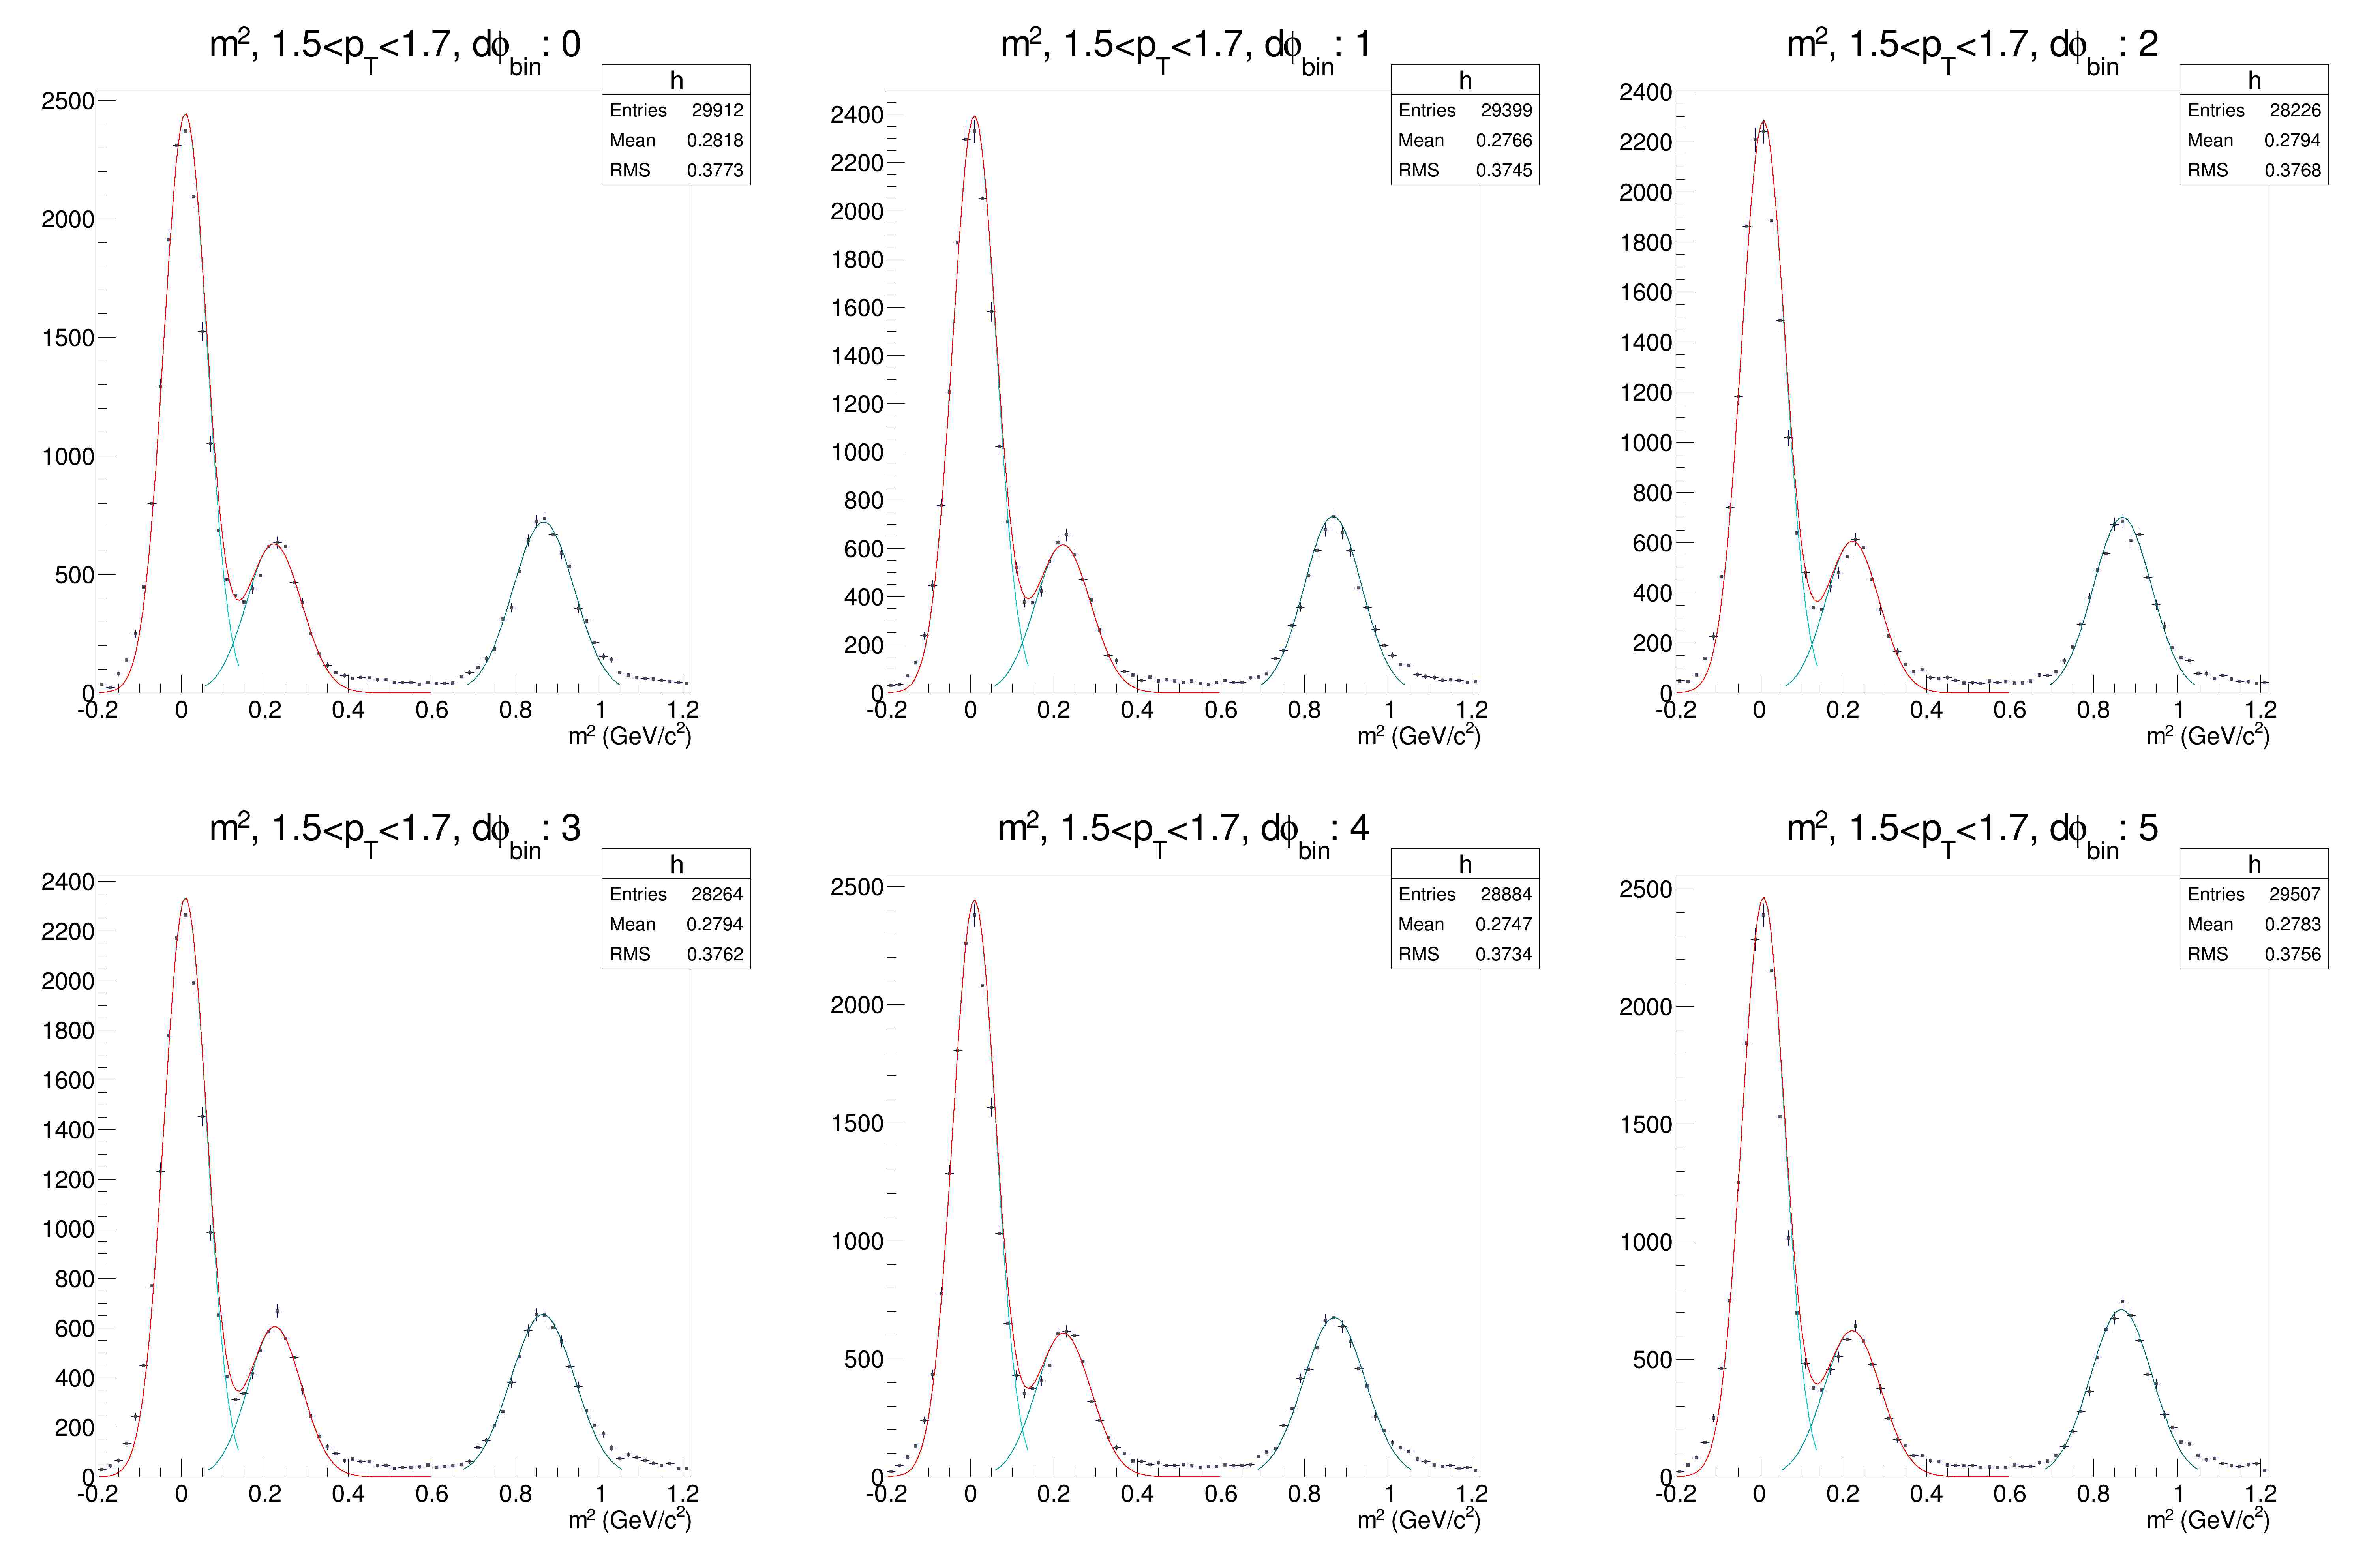
\includegraphics[width=1\textwidth]{lowptfits/yieldvsdphi_tof1_cent0_ch1_pT-15-17.jpg}
    \end{subfigure}
    \begin{subfigure}[p]{1\textwidth}
    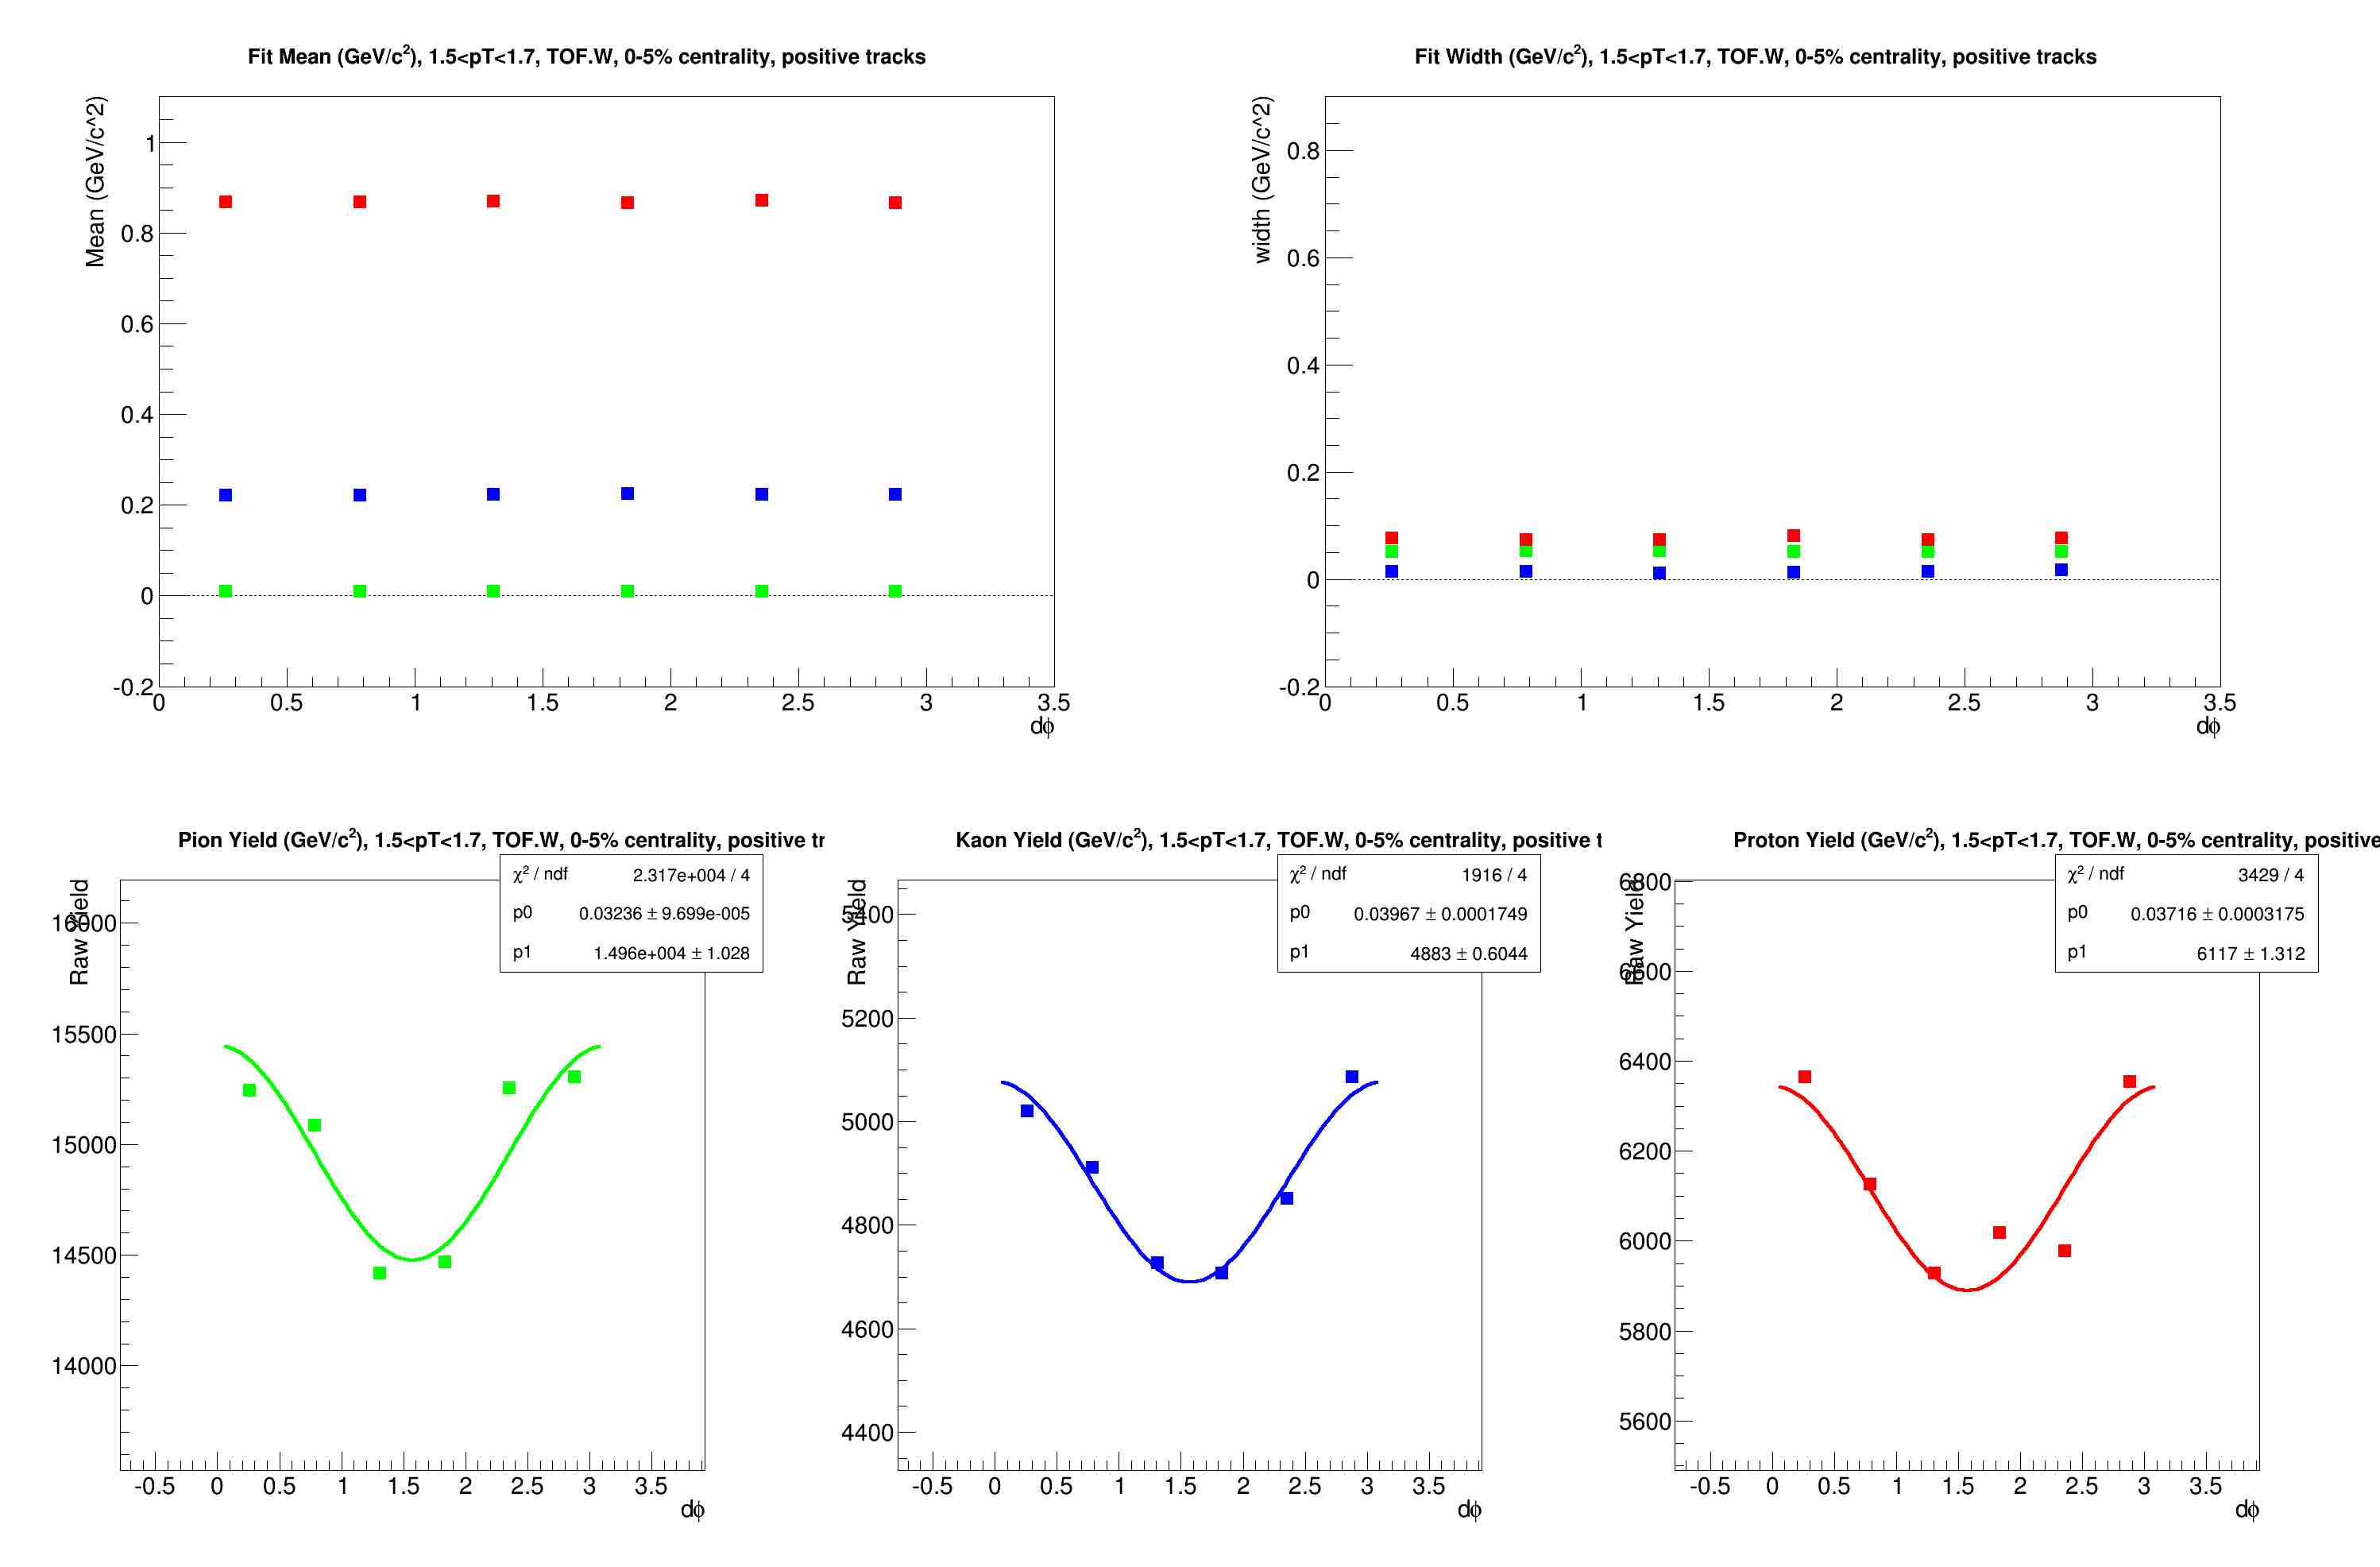
\includegraphics[width=1\textwidth]{lowptfits/fitParams_tof1_cent0_ch1_pT-15-17.jpg}
    \end{subfigure}
    \rule{35em}{0.5pt}
  \caption[PID fits and Yield vs $d\phi$ for $p_T$=1.5-1.7 GeV/c, TOF.W, positive particles ]{$m^2$ Gaussian fits for PID and resulting Yield vs $d\phi$ for $p_T$=1.5-1.7 GeV/c, TOF.W, positive particles}
  \label{fig:fits15-17pos}
\end{figure}

\begin{figure}[H]
  \centering
    \begin{subfigure}[p]{1\textwidth}
    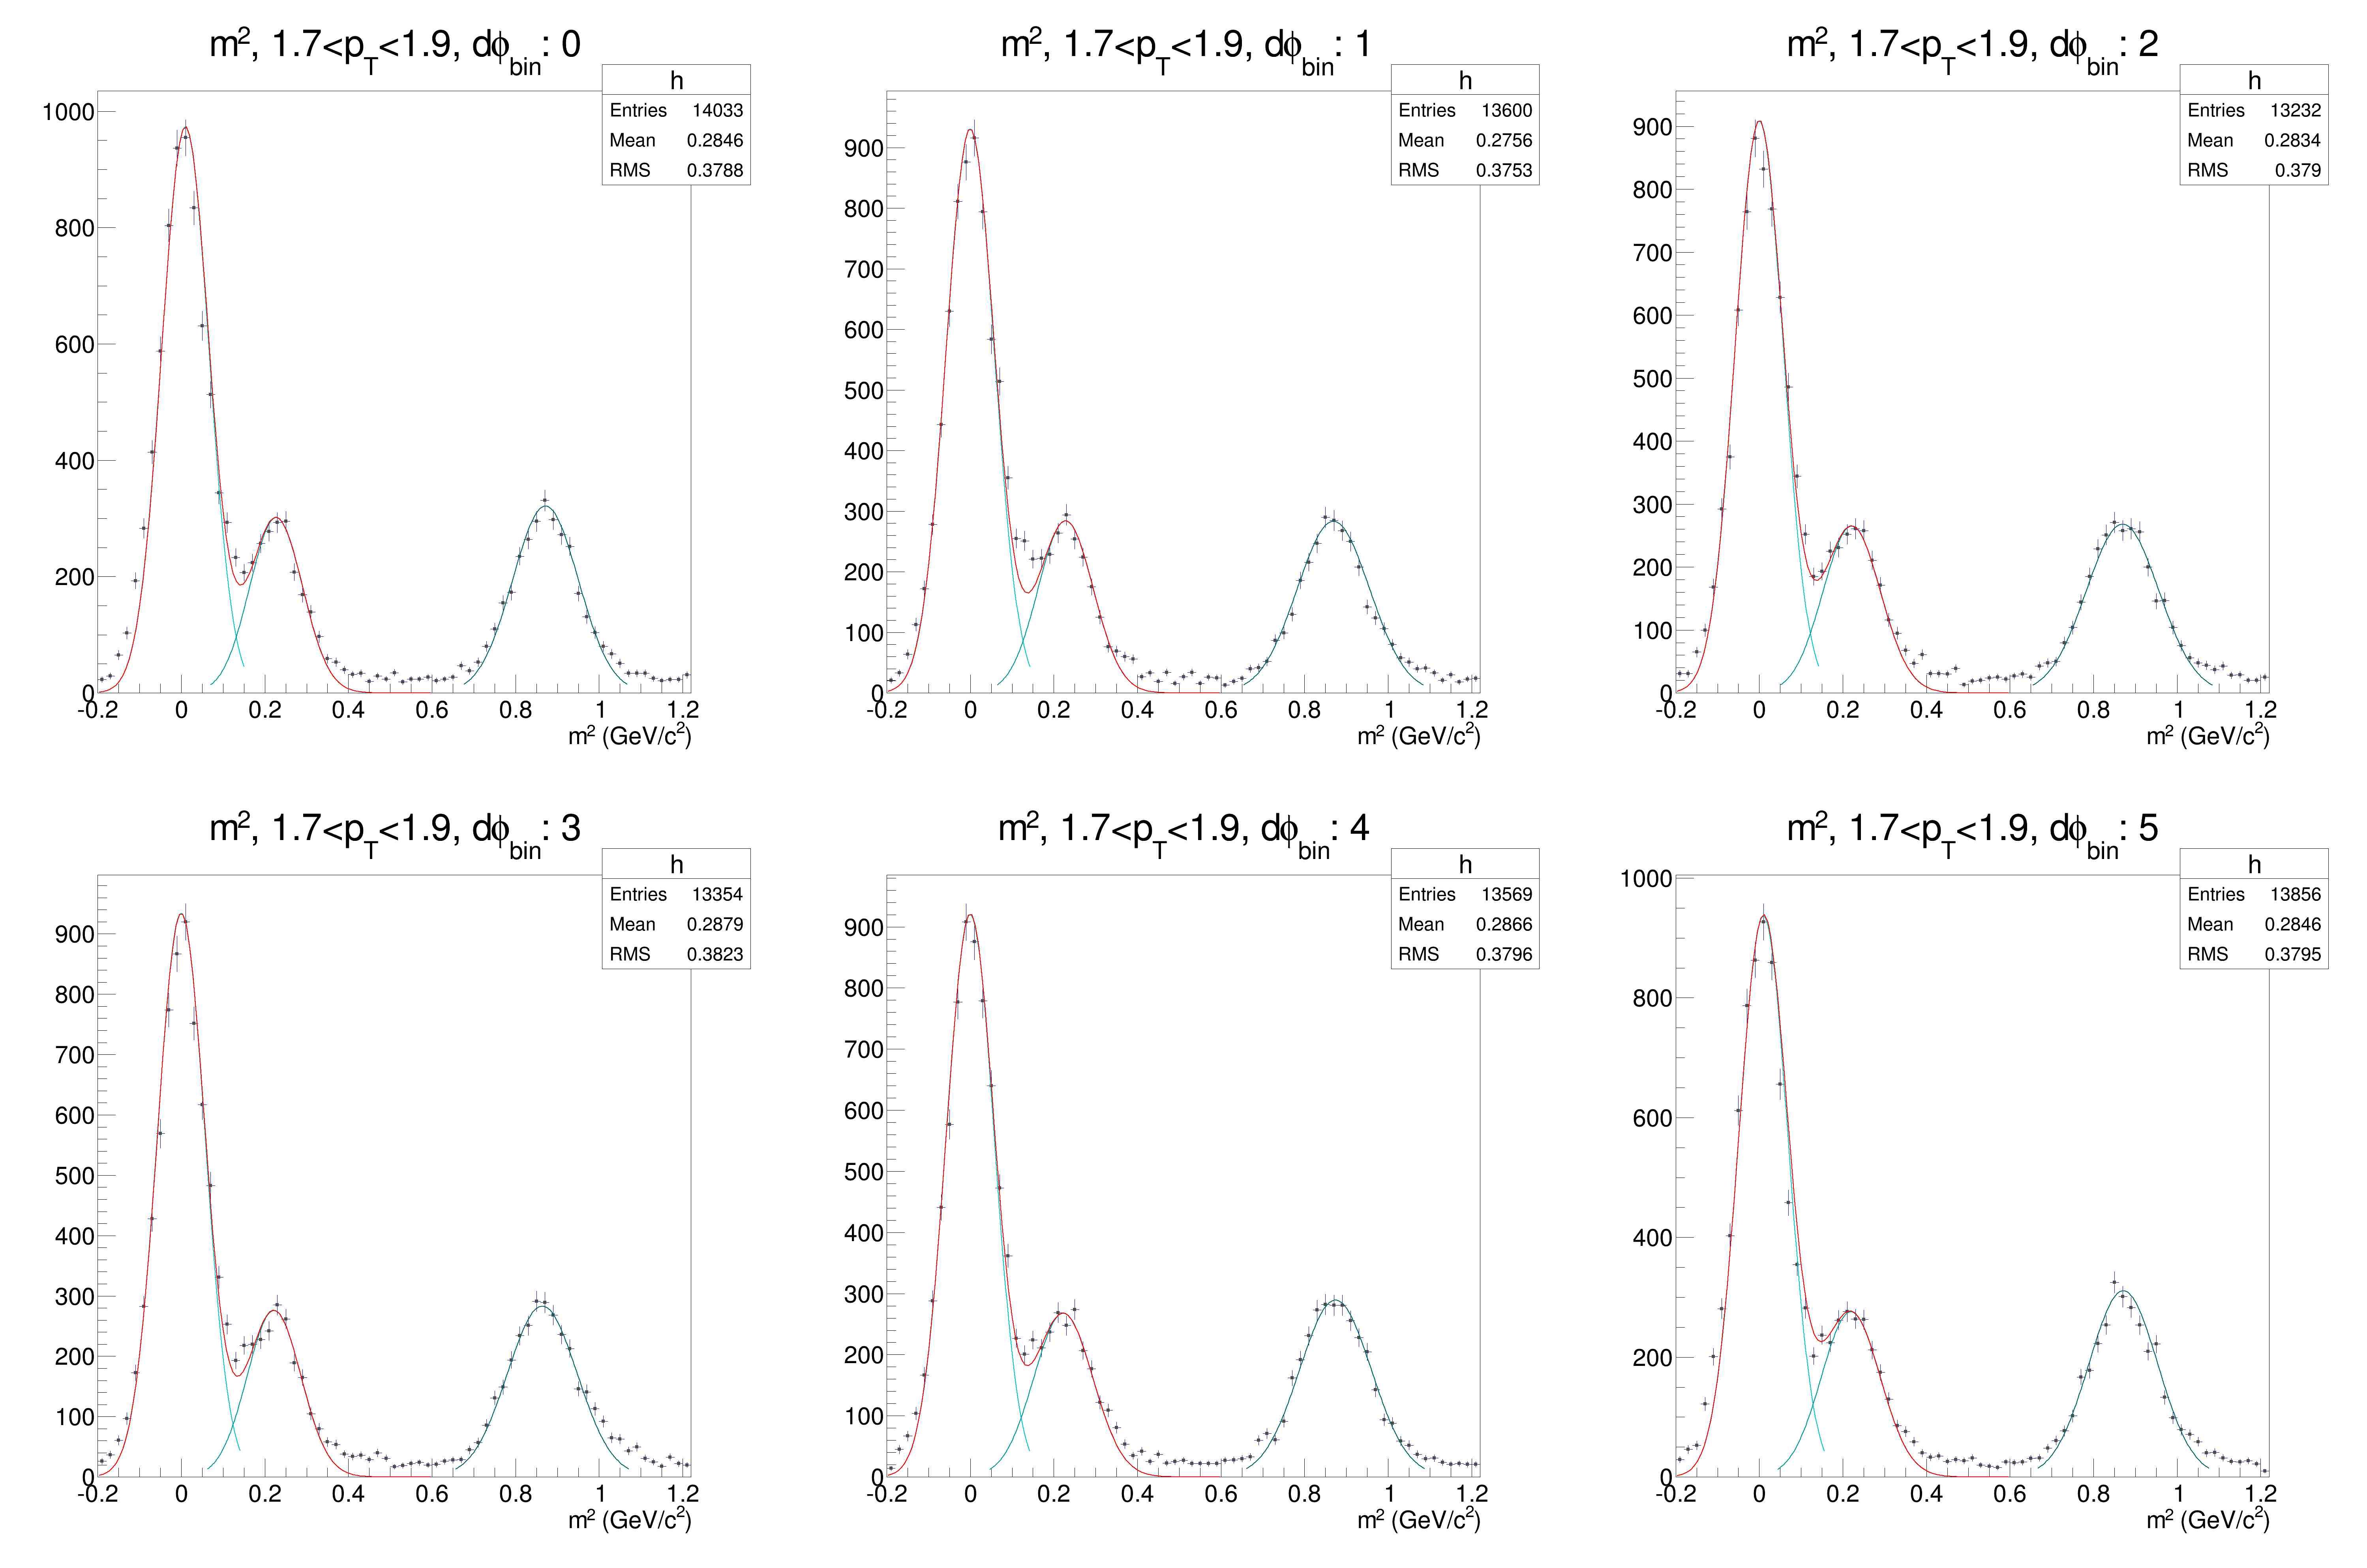
\includegraphics[width=1\textwidth]{lowptfits/yieldvsdphi_tof1_cent0_ch1_pT-17-19.jpg}
    \end{subfigure}
    \begin{subfigure}[p]{1\textwidth}
    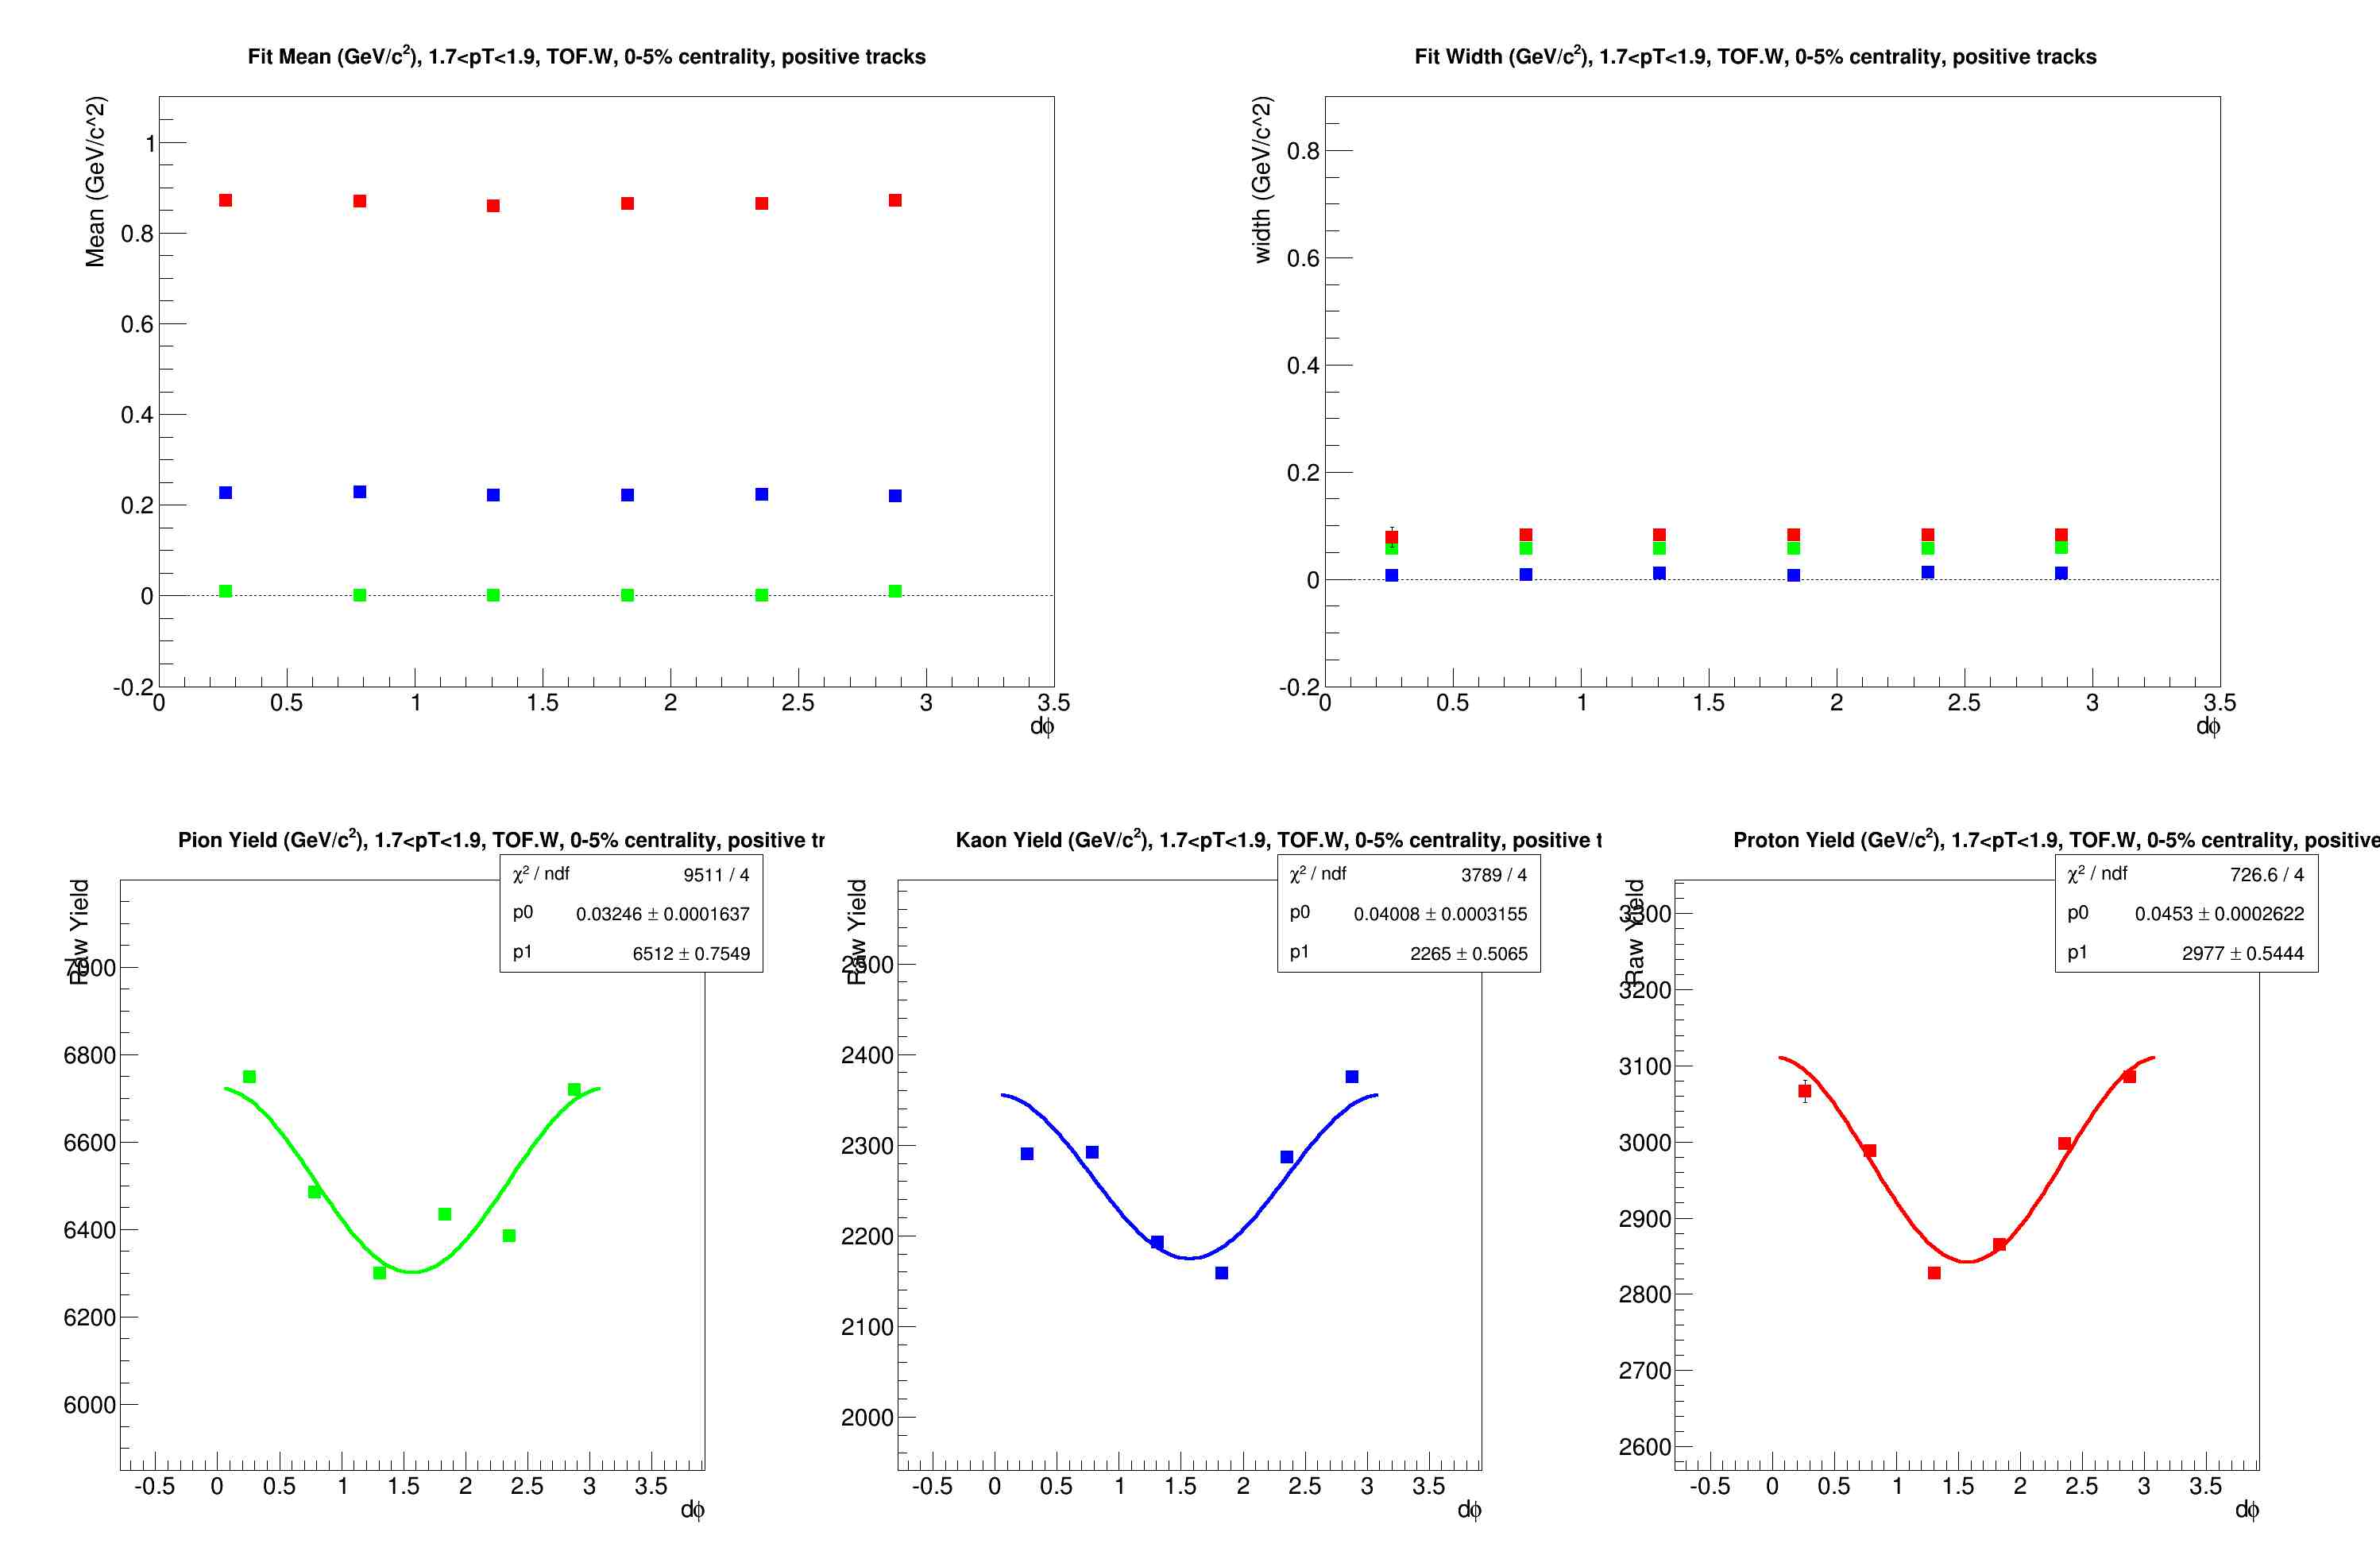
\includegraphics[width=1\textwidth]{lowptfits/fitParams_tof1_cent0_ch1_pT-17-19.jpg}
    \end{subfigure}
    \rule{35em}{0.5pt}
  \caption[PID fits and Yield vs $d\phi$ for $p_T$=1.7-1.9 GeV/c, TOF.W, positive particles ]{$m^2$ Gaussian fits for PID and resulting Yield vs $d\phi$ for $p_T$=1.7-1.9 GeV/c, TOF.W, positive particles}
  \label{fig:fits17-19pos}
\end{figure}

\begin{figure}[H]
  \centering
    \begin{subfigure}[p]{1\textwidth}
    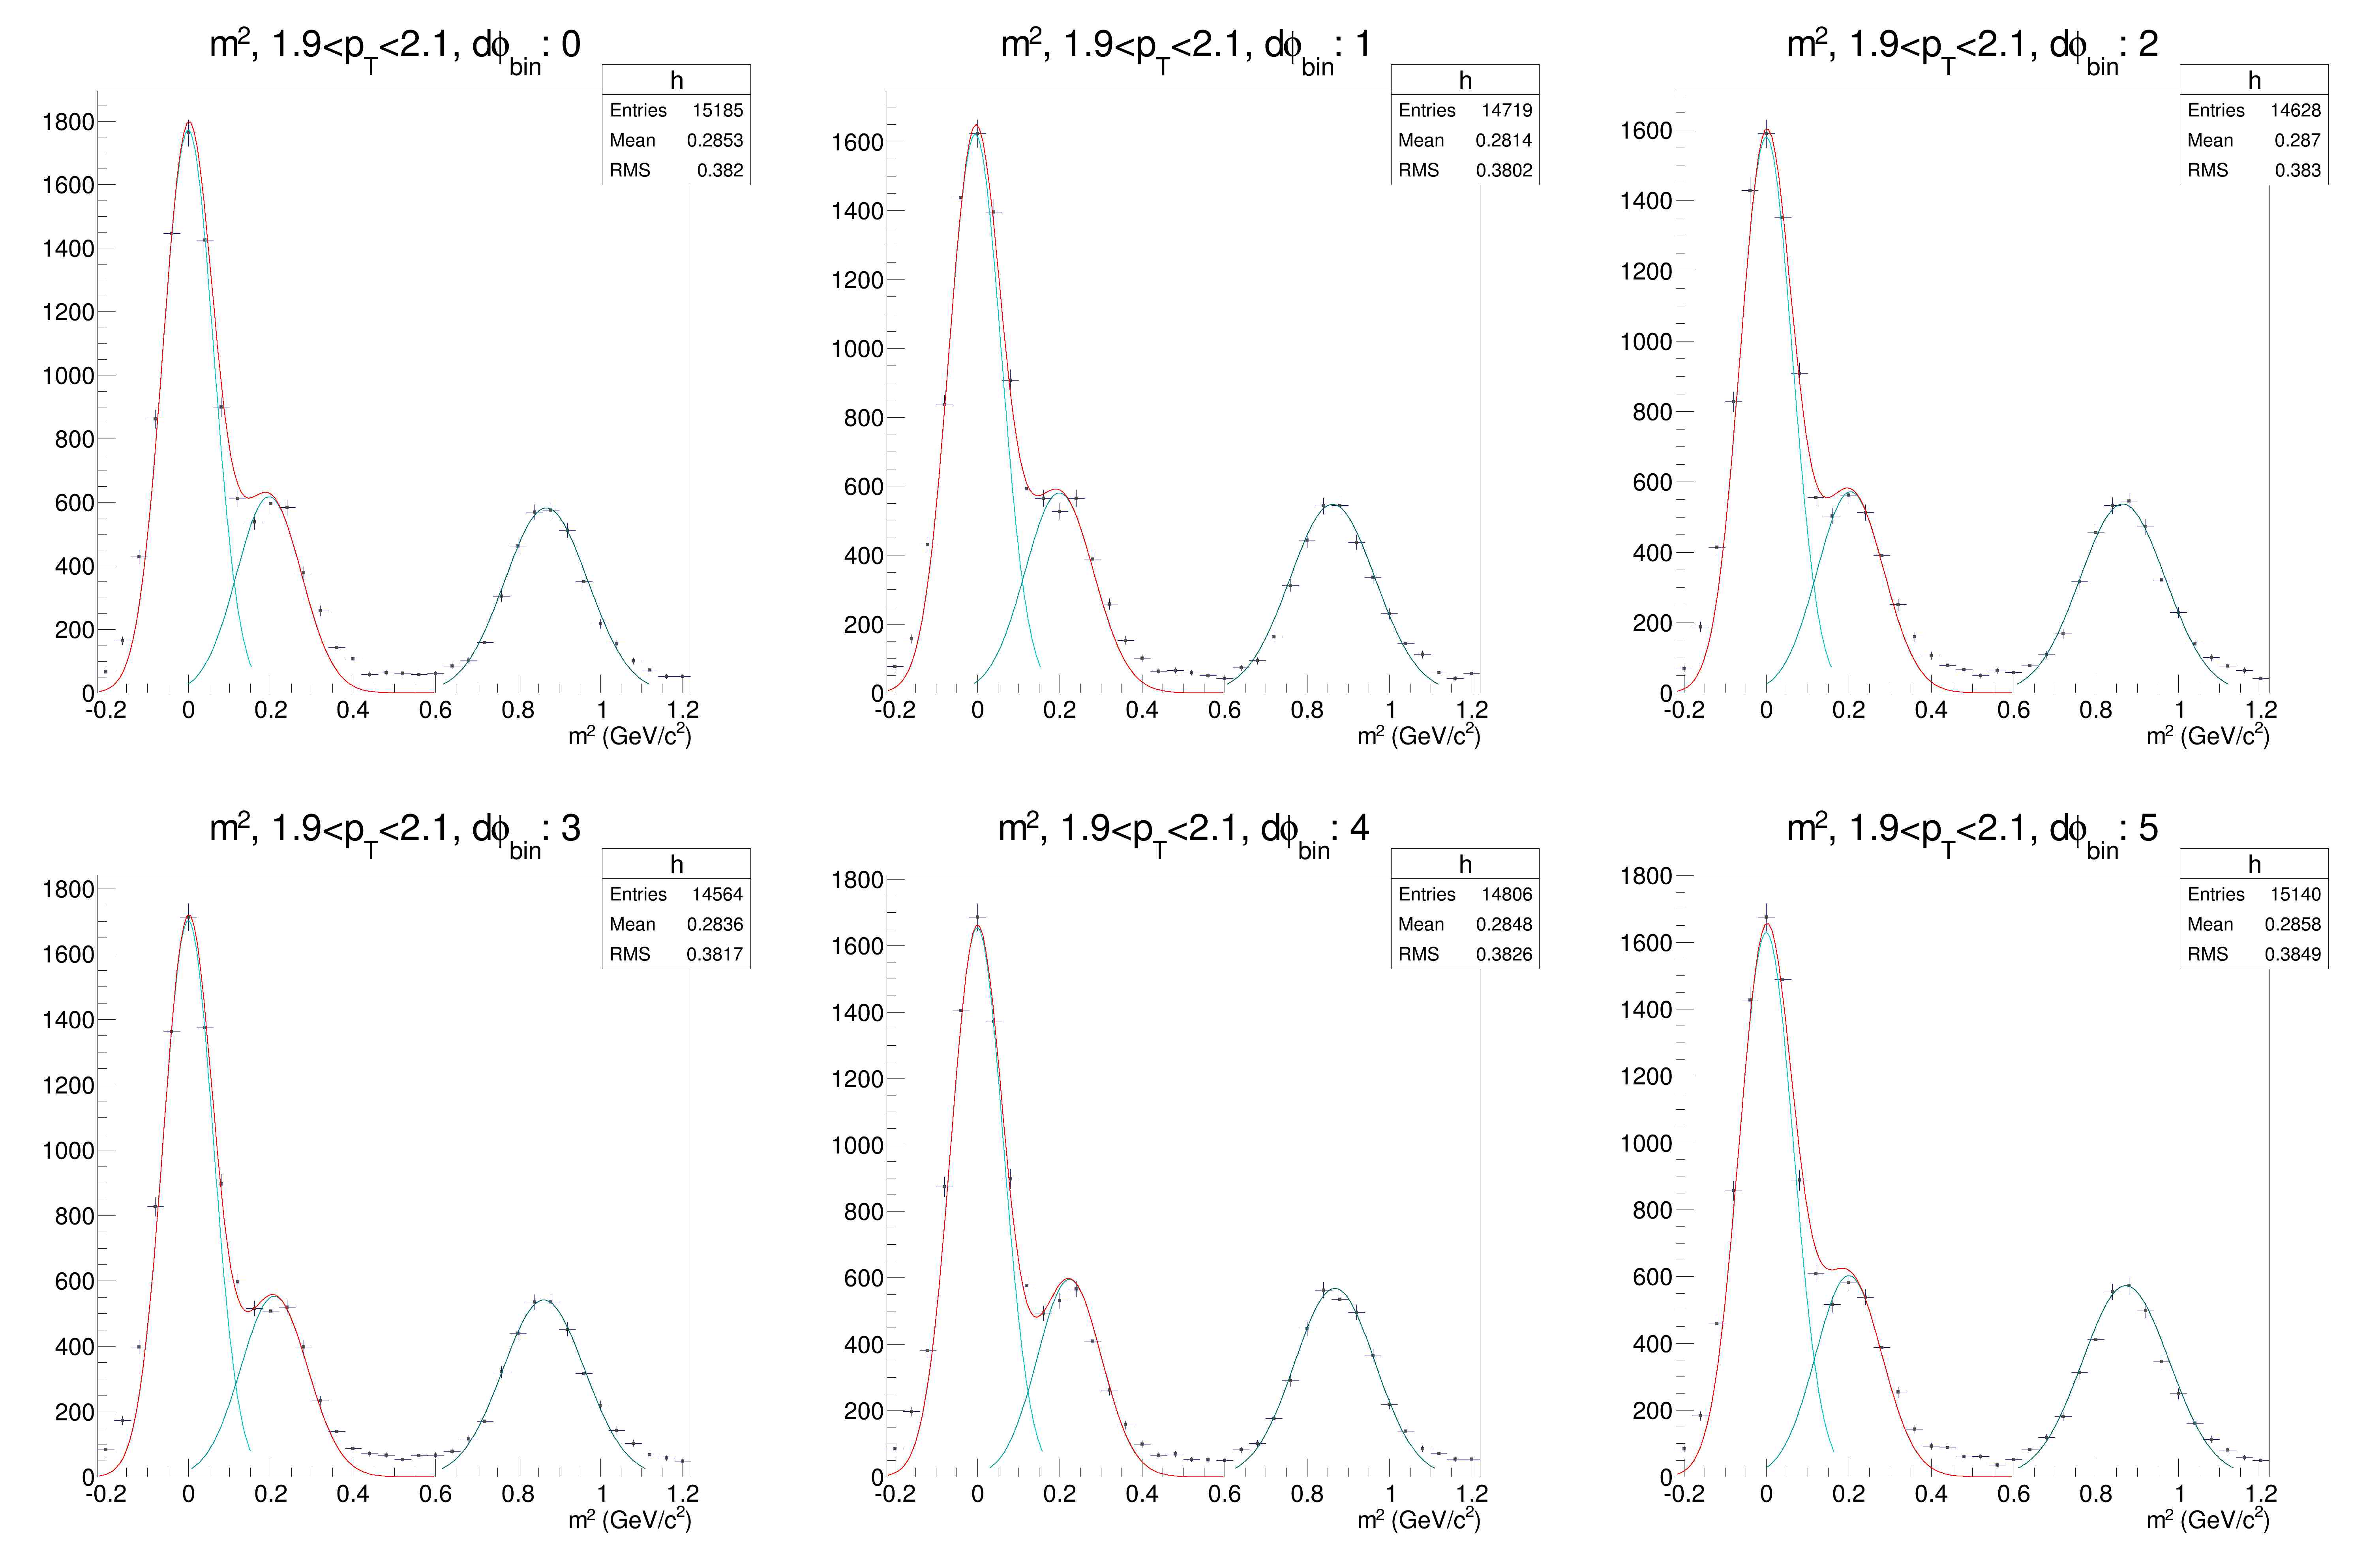
\includegraphics[width=1\textwidth]{lowptfits/yieldvsdphi_tof1_cent0_ch1_pT-19-21.jpg}
    \end{subfigure}
    \begin{subfigure}[p]{1\textwidth}
    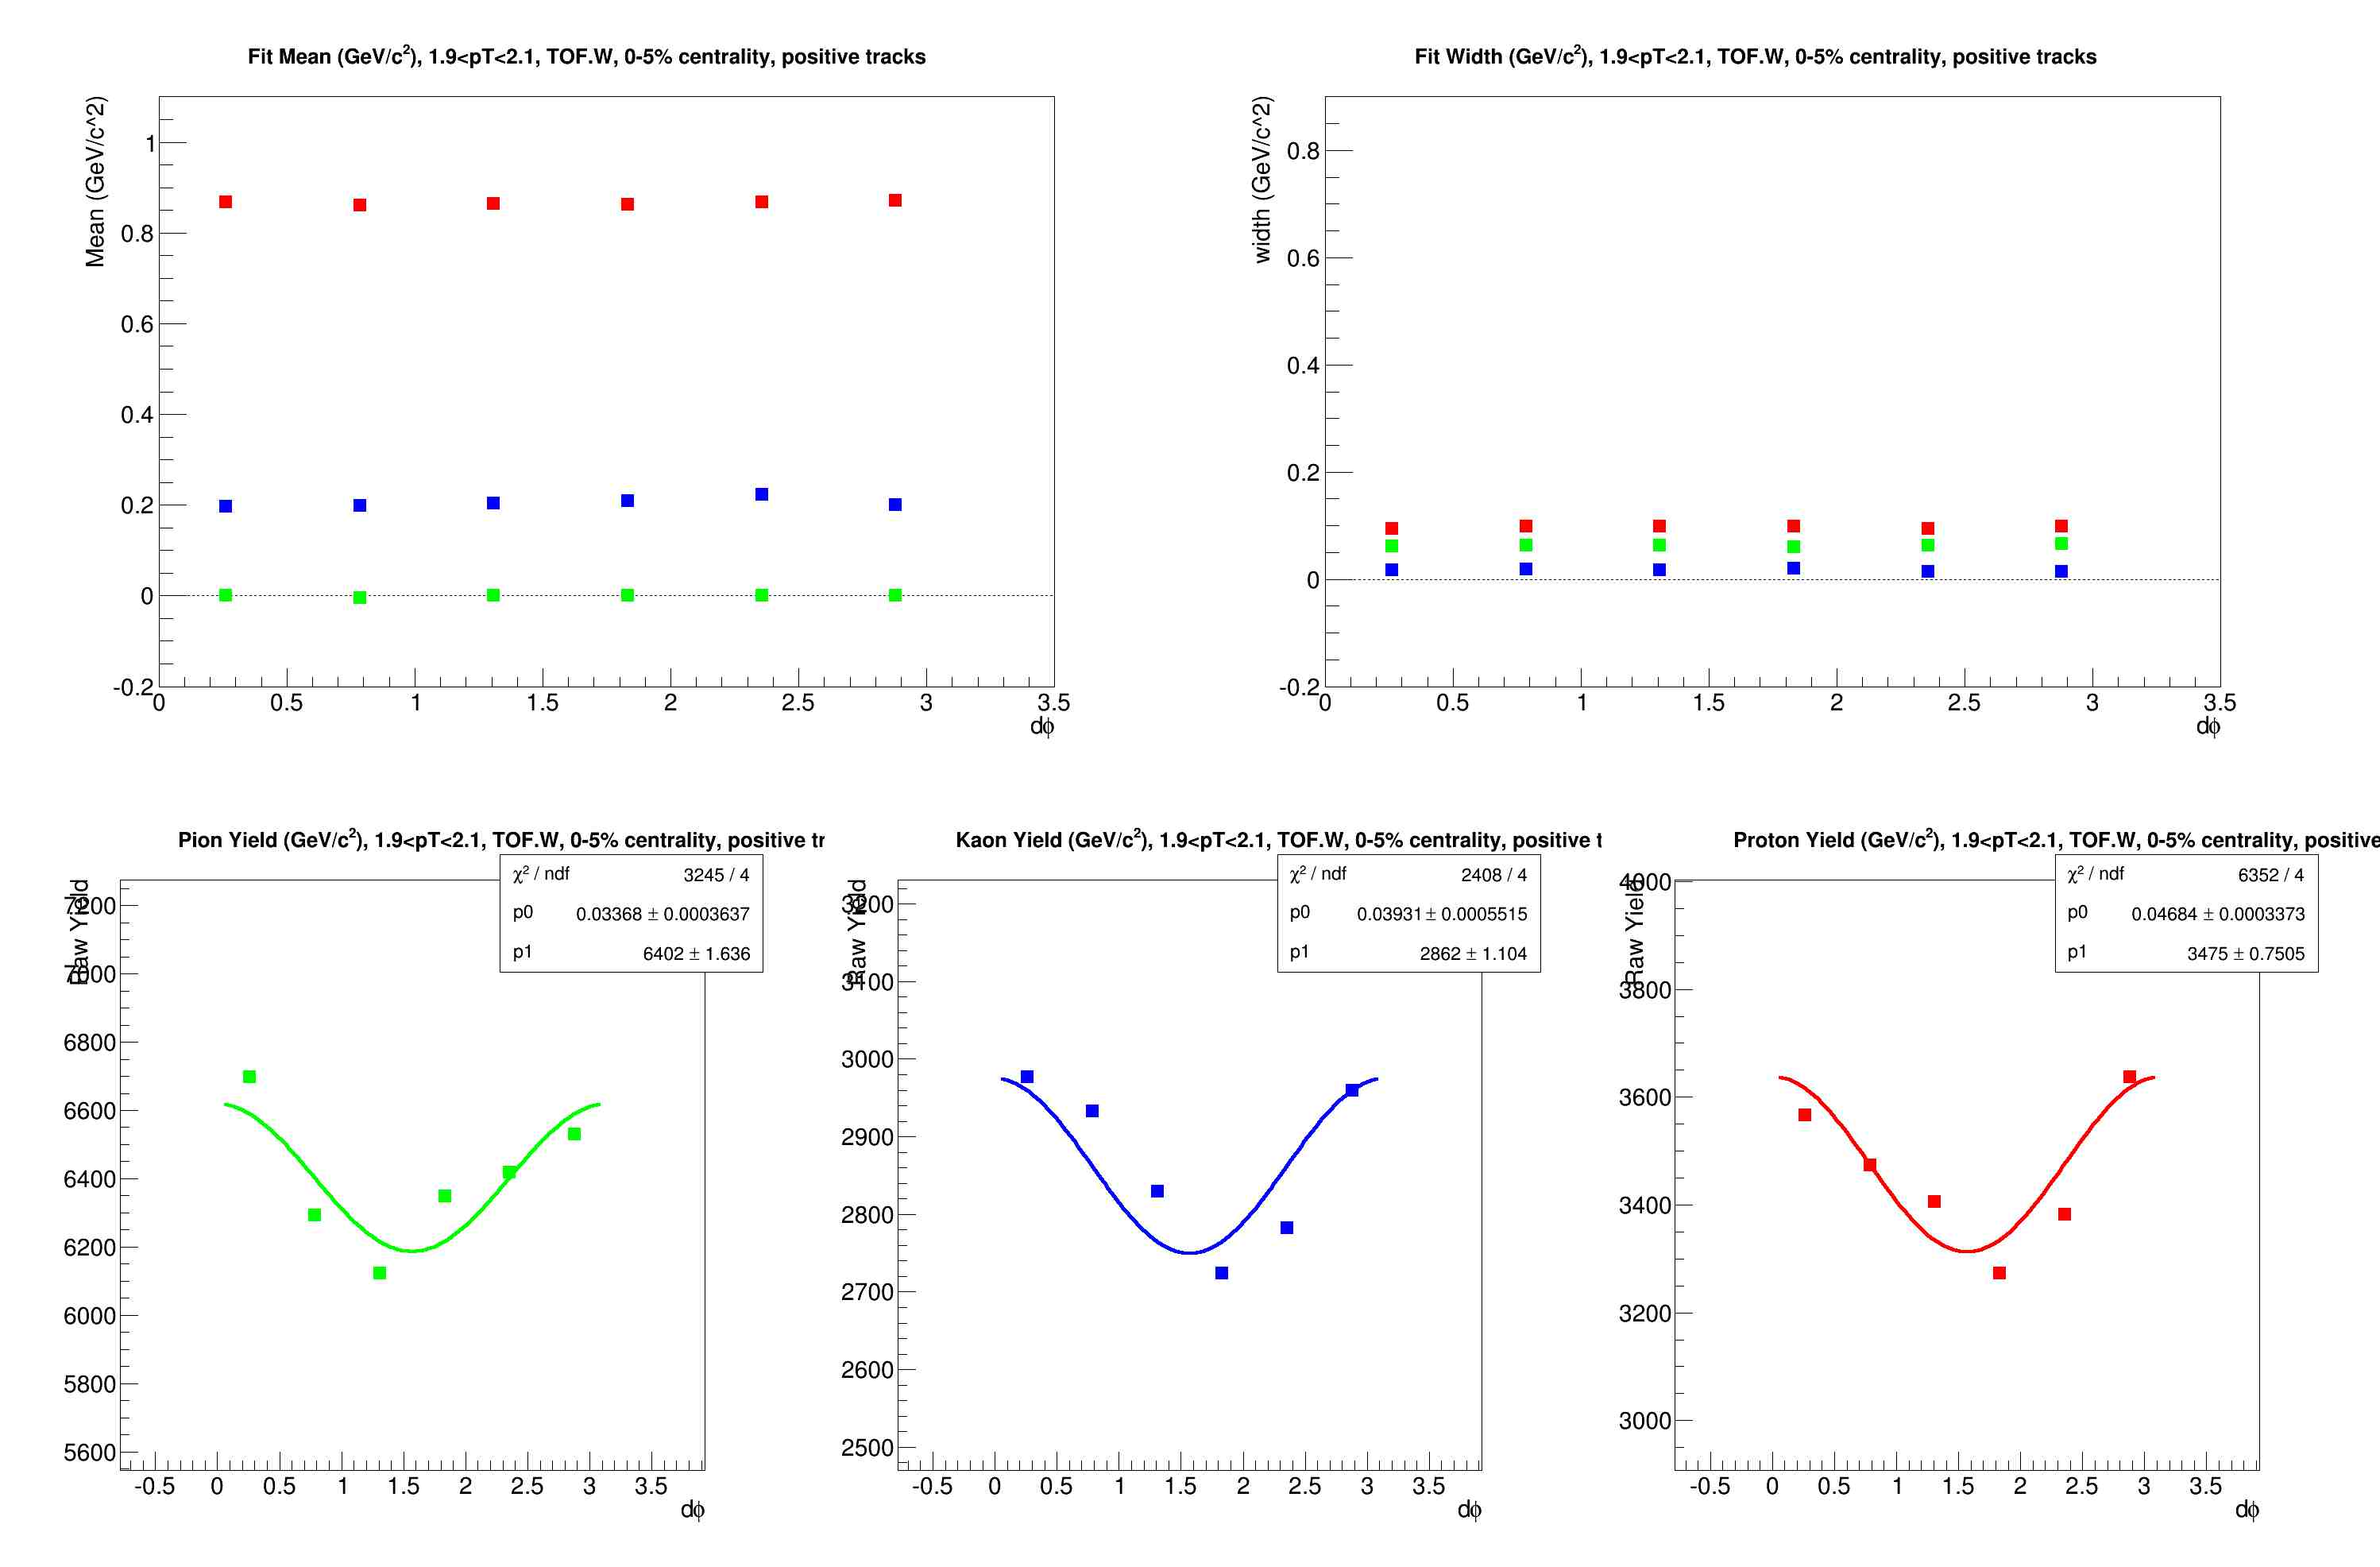
\includegraphics[width=1\textwidth]{lowptfits/fitParams_tof1_cent0_ch1_pT-19-21.jpg}
    \end{subfigure}
    \rule{35em}{0.5pt}
  \caption[PID fits and Yield vs $d\phi$ for $p_T$=1.9-2.1 GeV/c, TOF.W, positive particles ]{$m^2$ Gaussian fits for PID and resulting Yield vs $d\phi$ for $p_T$=1.9-2.1 GeV/c, TOF.W, positive particles}
  \label{fig:fits19-21pos}
\end{figure}
\restoregeometry

\subsection{ACC as a Particle Discriminator}
Above $p_T=2.3$ pion/kaon mixing becomes inseparable. In this region I utilize the ACC to trigger and veto pion and kaon events respectively by setting Cherenkov radiation threshold which is done by counting the number of photoelectrons collected by the two PMTs on each channel of the ACC. This utilization of the ACC therefore sorts tracks into two separate histograms, one with an \textit{ACC fire} condition that contains mostly pions with minimal kaon contamination, and another with an \textit{ACC veto} condition that contains the remaining kaons and protons with minimal pion contamination. These two histograms can then be analyzed with single Gaussians since the distributions are now separate.

\section{Yield vs Event Plane}
Here the yield vs $d\phi$ plots can be treated like the $dN/d\phi$ vs $d\phi$ plots that provided the charged track $v_2$ measurement which was acquired by fitting with the functional form of equation \ref{v2fitfn}. 
\section{Identified Particle $v_{2}$}

\pagebreak
\pagebreak
